\documentclass[openany,svgnames]{book}
\usepackage[svgnames]{xcolor}
\usepackage{blindtext}

\usepackage{comment}

\usepackage{cprotectinside}
\usepackage{ulem}

\usepackage{parskip}
%\setlength{\parindent}{0pt}
\setlength{\parindent}{0pt}

\usepackage{geometry}
\geometry{letterpaper, portrait, margin=0.5in}

\usepackage{imakeidx}
\makeindex[columns=3]

\usepackage{multicol}
\usepackage{enumitem}
\usepackage{tabularx}
\usepackage{nameref}
\usepackage{tikz}
\usepackage[sfdefault]{roboto}
\usepackage[most]{tcolorbox}
\tcbuselibrary{breakable}
\tcbuselibrary{skins}
\usepackage{booktabs}
\usepackage{xtab}
\usepackage{makecell}
\usepackage{wrapfig}

\usepackage{array,ragged2e}

\usepackage{titlesec}

\usepackage{etoolbox}

\usepackage{xparse}

\usepackage{ifthen}

\newcolumntype{L}{>{\RaggedRight\arraybackslash}X}
\newcolumntype{Y}{>{\raggedleft\arraybackslash}X}

\def\defcolwidth{0.6cm}
\def\aq{\textbf{Adventure Quest }}

\setcounter{secnumdepth}{5}

\DeclareDocumentCommand \indy { o m } {%
  \IfNoValueTF {#1} {%
    \lowercase{\def\temp{#2}}%
    %\def\temp{#2}%
    \index{\temp}%
    \textbf{#2}\xspace%
  }{%
    \lowercase{\def\temp{#1}}%
    %\def\temp{#1}%
    \index{\temp}%
    \textbf{#2}\xspace%
  }%
}

\DeclareDocumentCommand \indx { m } {%
    \lowercase{\def\temp{#1}}%
    \index{\temp}%
}

\newcommand{\bhead}[1]{\thead{\textbf{#1}}}
%\newcommand{\defnum}[1]{\underline{\textbf{#1}}}
\newcommand{\defnum}[1]{\uline{\textbf{#1}}}
\newcommand{\mets}[4]{%
  \ifthenelse{\equal{#2}{}}{%
    \defnum{#1 mets} (\textit{#3 mi or #4 KM})%
  }%
  {%
    \defnum{#1 mets} per #2 (\textit{#3 mi or #4 KM})%
  }
}

\newcommand{\chref}[1]{\textbf{Chapter \ref{#1}: \nameref{#1}}}
%\textbf{Chapter \ref{ch:jaern-humanoids}: \nameref{ch:jaern-humanoids}}

\setlength\intextsep{0pt}

\newlength{\doublemulticol}
\setlength{\doublemulticol}{0.25cm}

\setlength{\multicolsep}{0pt}%


\DeclareRobustCommand{\STR}{\indy[strength!STR]{STR}}
\DeclareRobustCommand{\INT}{\indy[intelligence!INT]{INT}}
\DeclareRobustCommand{\PER}{\indy[perception!PER]{PER}}
\DeclareRobustCommand{\CSE}{\indy[common sense!CSE]{CSE}}
\DeclareRobustCommand{\HEA}{\indy[health!HEA]{HEA}}
\DeclareRobustCommand{\AGI}{\indy[agility!AGI]{AGI}}
\DeclareRobustCommand{\PWR}{\indy[power!PWR]{PWR}}
\DeclareRobustCommand{\COM}{\indy[comliness!COM]{COM}}
\DeclareRobustCommand{\WIL}{\indy[willpower!WIL]{WIL}}
\DeclareRobustCommand{\DV}{\indy[weapon!defensive value]{DV}}
\DeclareRobustCommand{\CDV}{\indy[combat defense!CDV]{CDV}}
\DeclareRobustCommand{\CM}{\indy[combat modifier!CM]{CM}}
\DeclareRobustCommand{\GDV}{\indy[grapple defense!GDV]{GDV}}
\DeclareRobustCommand{\GM}{\indy[grapple modifier!GM]{GM}}
\DeclareRobustCommand{\MDV}{\indy[missile defense!MDV]{MDV}}
\DeclareRobustCommand{\MM}{\indy[missile modifier!MM]{MM}}
\DeclareRobustCommand{\DP}{\indy[damage points!DP]{DP}}
\DeclareRobustCommand{\EP}{\indy[experience points!EP]{EP}}
\DeclareRobustCommand{\DU}{\indy[divine units!DU]{DU}}
\DeclareRobustCommand{\EU}{\indy[elemential units!EU]{EU}}
\DeclareRobustCommand{\LF}{\indy[life force!LF]{LF}}
\DeclareRobustCommand{\LOS}{\indy[line of sight!LOS]{LOS}}
\DeclareRobustCommand{\RC}{\indy[resistance check!RC]{RC}}
\DeclareRobustCommand{\DI}{\indy[divine intervention!DI]{DI}}
\DeclareRobustCommand{\ADV}{\indy[Artillery Defense Value!ADV]{ADV}}

\newcommand{\newacronymidx}[4][]{
    \newacronym{#2}{#3}{#4}
    \ifstrempty{#1}
        { \index{#3|see{\MakeLowercase{#4}}} }
        { \index{#3|see{#1}} }
}

\DeclareTotalTCBox{\tcdieroll}{ O{GreenYellow} v !O{} }{%
  leftrule=0mm,%
  rightrule=0mm,%
  toprule=0mm,%
  bottomrule=0mm,%
  rounded corners,%
  top=0pt,%
  bottom=0pt,%
  left=2pt,%
  right=2pt,%
  tcbox raise base,%
  boxsep=0mm,%
  nobeforeafter,%
  colback=white!40!#1,%
  colupper=black,%
  halign=center,%
  }{\textbf{\strut{#2}}}

\DeclareTotalTCBox{\tcdefine}{ O{DodgerBlue} v !O{} }{%
  leftrule=0mm,%
  rightrule=0mm,%
  toprule=0mm,%
  bottomrule=0mm,%
  rounded corners,%
  top=0pt,%
  bottom=0pt,%
  left=2pt,%
  right=2pt,%
  tcbox raise base,%
  boxsep=0mm,%
  nobeforeafter,%
  colback=white!30!#1,%
  colupper=black,%
  halign=center,%
  }{\textbf{\strut{#2}}}

\DeclareTotalTCBox{\tcpage}{ O{Crimson} m !O{} }{%
  leftrule=0mm,%
  rightrule=0mm,%
  toprule=0mm,%
  bottomrule=0mm,%
  rounded corners,%
  top=0pt,%
  bottom=0pt,%
  left=2pt,%
  right=2pt,%
  tcbox raise base,%
  boxsep=0mm,%
  nobeforeafter,%
  colback=white!50!#1,%
  colupper=black,%
  halign=center,%
  }{\strut{\textbf{Page \pageref{#2}}}}

\newtcolorbox{normbox}[1][]{%
  boxrule=0pt,%
  enhanced,%
  title=\textbf{#1},%
  left=2pt,%
  right=2pt,%
  top=2pt,%
  bottom=1pt,%
  boxsep=2pt,%
  boxrule=0.6pt,%
  before skip=0.5\baselineskip,%
  lefttitle=2mm,%
  righttitle=2mm,
  toptitle=1mm,%
  bottomtitle=1mm,%
  minipage boxed title,%
  hbox,%
  colbacktitle=Navy,%
  colback=white,%
  }

\newtcolorbox{normboxw}[1][]{%
  boxrule=0pt,%
  enhanced,%
  title=\textbf{#1},%
  left=2pt,%
  right=2pt,%
  top=2pt,%
  bottom=1pt,%
  boxsep=2pt,%
  boxrule=0.6pt,%
  before skip=0.5\baselineskip,%
  lefttitle=2mm,%
  righttitle=2mm,
  toptitle=1mm,%
  bottomtitle=1mm,%
  minipage boxed title,%
  width=\columnwidth,%
  colbacktitle=Navy,%
  colback=white,%
  }

\newtcolorbox{normboxper}[2][]{%
  boxrule=0pt,%
  enhanced,
  title=\textbf{#2},%
  left=2pt,%
  right=2pt,%
  top=2pt,%
  bottom=1pt,%
  boxsep=2pt,%
  boxrule=0.6pt,%
  lefttitle=2mm,%
  righttitle=2mm,
  toptitle=1mm,%
  bottomtitle=1mm,%
  width=#1\linewidth,%
  %width=0.5\linewidth,%
  minipage boxed title,%
  %attach boxed title to top,%
  colbacktitle=Navy,%
  colback=white,%
  }

\hyphenpenalty=5000


\begin{document}
\enlargethispage{1.5\baselineskip}
\titleformat{\chapter}[display] {\normalfont\huge\bfseries}{\chaptertitlename\ \thechapter}{20pt}{\Huge}   
\titlespacing*{\chapter}{0pt}{20pt}{40pt}
\titlespacing\section{0pt}{6pt}{6pt}
\titlespacing\subsection{0pt}{6pt }{6pt}
\titlespacing\subsubsection{0pt}{6pt}{6pt}
%\begin{comment}
\savebox{\this}{
\begin{normbox}[Test]
\blindtext
\end{normbox}
}
\settowidth{\thislen}{\usebox{\this}}
\printlength{\thislen}

\begin{wrapbox}[10cm]
\begin{normbox}[TEST]
%\usebox{\this}%
\blindtext
\end{normbox}
\end{wrapbox}
Lorem Ipsum is simply dummy text of the printing and typesetting industry. Lorem Ipsum has been the industry's standard dummy text ever since the 1500s, when an unknown printer took a galley of type and scrambled it to make a type specimen book. It has survived not only five centuries, but also the leap into electronic typesetting, remaining essentially unchanged. It was popularised in the 1960s with the release of Letraset sheets containing Lorem Ipsum passages, and more recently with desktop publishing software like Aldus PageMaker including versions of Lorem Ipsum.
\end{comment}

\begin{comment}
\indy{TESTI}

\large
\bfseries
\itshape
TEST\\
\makeatletter
\f@size

\f@shape

\f@series
\makeatother\\
\the\textwidth

\indy[aaa]{TESTI2}

\the\tabcolsep
\end{comment}

\begin{titlepage}
\begin{center}
\huge Adventure Quest\\
Jaern\\
\vspace*{1cm}
\normalsize a Role Playing System\\
\vspace*{1cm}
created by\\
Daniel Lawrence\\
\vspace*{1cm}
based on version published\\
April 5th, 2010\\
\vspace*{1cm}
modified by\\
Michael Lubert\\
\vspace*{1cm}
modified version publish date\\
\today
\end{center}
\end{titlepage}
First Edition

\vspace*{1cm}
\begin{tabular}{ l l }
First Printing: & July 1991\\
Second Printing: & September 1992\\
Third Printing: & November 1992\\
Fourth Printing: & September 1997\\
Fifth Printing: & August 1998\\
Sixth Printing: & July 1999\\
Seventh Printing: & March 2001\\
Eigth Printing: & August 2005
\end{tabular}

\vspace*{1cm}
Copyright 1989 – 2010 by Daniel M. Lawrence and Robert J. Blake\\
Copyright 2010-2024 by Greg Mowczko

\vspace*{0.5cm}
All Rights are reserved. No part of this publication may be reproduced, stored in a retrieval system, or transmitted, in any form, or by any means, electronic, photocopying, recording, or otherwise, without prior written permission of the publisher.

\vspace*{1cm}
Published by Daniel M. Lawence and Robert J. Blake\\
Adventure Quest is a trademark owned by Daniel M. Lawrence

\vspace*{1cm}
Find\\
http://www.aquest.com/\\
on the Internet to recieve up to date information on all Adventure Quest games.
\textbf{\huge Dedication}

This game is dedicated to the memory of Robert J. Blake, whom did so much to further the art and the fun of roleplaying.
You will be sorely missed.

This is also dedicated to Daniel M. Lawrence, who brought this game to life for so many.
\textbf{INTRODUCTION}

\textbf{Adventure Quest\textsuperscript{TM}} (\textbf{AQ} for short) is a role playing system in which you, through your game persona (adventurer), can experience all the thrills and perform deeds of derring-do in a fantasy world. It is like being the hero in an adventure novel, only, instead of just reading about what happens, your actions and decisions direct the storyline. You can destroy evil maidens, rescue fair dragons, or even be a knight in very dull armor. Your imagination is the only limit to what you can do while playing Adventure Quest.

As a player, you create an adventurer which you control. Another person, called the Game Master (GM), presents to you and other players a fantasy world of cities, towns, creatures, oppressive overlords, demanding temples, and lots of magic and treasure. You tackle adventures in this world to satisfy the personality and motives of your adventurer. Adventure Quest tm provides adventure in a variety of different settings (Games), each with its own history, customs, inhabitants, villains, and deities. 

This Game covers adventuring in JAERN, a distant fantasy world far in our future. Other Adventure Quest games include AQ/BRITANNIA, describing a world similar to the British Isles in t he mid 1200’s; AQ/KHEMET, providing adventure in a land akin to ancient Egypt; AQ/FREEZONE, a coorporate ruled gangland in the near future; and AQ/SPACE, for adventuring in the outer reaches of Interstellar Space among the Pan-Human Hegemony.

\textbf{Realism and Playability}

Adventure Quest/Jaern is a complete game; you do not have to buy any other books before beginning play. It contains all the necessary information for players to create and play their adventurers, and for Game Masters to design and maintain a campaign. Any game such as this must strike some kind of balance between realism and playability. The mechanics used in this manual lean heavily towards the latter, with the idea that you should spend your time roleplaying your creations, be you a player or Game Master, rather than wading through very complex rules for the sake of realism.

That said, we realize that some of you might be willing to make a different tradeoff. Where appropriate, optional rules are included offering different, but more complex, mechanics that arguably provide greater realism. The players and Game Master may choose which options to include to tailor the game to their liking. The cornerstone of \textbf{Adventure Quest\textsuperscript{TM}} games are flexibility. Much of the game book deals with the creation of personalities, creatures, magical items, etc. Examples are provided that you can use as is, but more importantly we tell you how to create your own that will automatically be balanced with the system.

\textbf{About Role Playing}

Playing Adventure Quest, like any role playing game, should be a fun and exciting experience. Your adventurer will likely encounter many unusual, exotic, and strange situations, people, and activities. Your adventurer may end up in conflict with, or allied to, an array of intelligent beings and creatures, many of which we might consider strange or even evil by today’s standard and mores. Please remember that this is "just a game." The authors in no way endorse or suggest that you act out any game-related actions or methods in the real world. Practice safe gaming, and leave the game and any enemies you make there behind you at the gaming table.

\textbf{How to Use this Book}
\begin{itemize}
\item All players and Game Masters should read Chapters 1 through 4 which deal with the creation and playing of adventurers.
\item Chapters 5 through 10 describe the world of Jaern, the setting for this game, and is therefore also pertinent for both players and Game Masters.
\item Chapters 11 through 27 present the magic available in AQ/Jaern. 
\begin{itemize}
\item Chapter 11 discusses nomadic mystiscism. 
\item Chapters 12 through 16 deal with elemental magic, and are therfore of primary interest to players whose adventurers use magician spells.
\item Chapters 17 through 27 deal with divine magic. Each deity has its own chapter, so these are of interest to any player whose adventurer follows a particular god or goddess.
\end{itemize}
\item Chapters 28 through 35 are meant primarily for the Game Master. They discuss creation of actors, creatures, and treasures, designing interesting and exciting adventures, adjudicating adventures, and how to maintain a campaign.
\end{itemize}

\textbf{Original Acknowledgements}

The list below is really just the beginning. Many people have contributed in different ways at different stages of this project. We would especially like to thank Mark Shoemaker for lots of zany ideas and style over many years, Bob Ferguson for his devotion in filling out thousands of forms, to Scott Delaney for fixing all our cars, to Tony Charlesworth for his endless time researching a world full of information, to Greg Mowzko for not letting a single error problem by no matter how insufferable it was, to Microsoft for their Access product that holds all of our databases, and to our good roleplaying friends in Lake Geneva, for providing us the motivation.

Robert J. Blake, my coauthor of this system, created most of the elemental spells, a lot of creatures, many skill descriptions and provided a sounding board for all the basic concepts behind our system. He provided endless encouragement to bring this project to pass. Robert ran the AD\&D Open Tournement at the Gencon Gaming convention for over a decade, overseeing uncountable details of scenario design and game master coordination. It was his experience which made it possible for us to create this system. Also our work on these concepts found its place in improving other systems in many ways. Sadly, we lost Robert at the beginning of the new millenium. He will be greatly missed.

\textbf{Design assistance:}\\
Daniel Lawrence\\
Robert J. Blake\\
Dana Hoggatt\\
Eric Delaney\\
Christopher Stanley\\
Steve Ames\\
Greg Mowczko

\begin{tabular}{ l l }
\textbf{Cover Art:} & Terry Pavlet\\
\textbf{Interior Art:} & Sean Cannon\\
 & Kirstein Jacobus\\
 & Scott Starkey\\
\textbf{Logo Design:} & Karen Klutzke\\
\textbf{Database Design:} & Daniel Lawrence\\
\end{tabular}

\textbf{Play Testers:}\\
\begin{tabular}{ l l l l }
Aaron K Alexander & Andrew Grey Smith & Andrew M Luers & Anthony C Brown\\
Anthony Charlesworth & Benjamin Wai & Bill Dorell & Brent D McLean\\
Brett Riester & Brian Cash & Calvin Krug & Charles Voelkel\\
Chris Esser & Daniel Lawrence & Terry Pavlet & Sean Cannon\\
Kirstein Jacobus & Scott Starkey & Karen Klutzke & Daniel Lawrence\\
Chris Normand & Craig Waylan & Dana Shea & David H Morse\\
David Moore & David Ward & Eric Starkey & Erich Shultz\\
Gregory Mowczko & Jeff Hartwig & Jim Ivey & Joe Gregorovich\\
Jose Berrios & John Flournoy & John Haley & John W. Fisher\\
John R. Prewitt III & Kat Price & Kathy Janney & Kirk Monsen\\
Lee Kenyon & Lyle H Janney & Mark Muller & Matthew W Somers\\
Michael Ballard & Michael Brobst & Patrick Collins & Patrick Perrone\\
Paul Bernard & Robert Tertocha & Robert Thelan & Robert Westerman\\
Ryan Gavigan & Ryan Parker & Scott Starkey & Sean L McLane\\
Steve Ames & Terran D Lane & Tessy E Fitzpatrick
\end{tabular}
\chapter{Creating an Adventurer}
\label{ch:create-adventurer}
\index{adventurer!creating}
To play in \textbf{Adventure Quest} (\textbf{AQ} for short), you must first create an adventurer to control during the game. All adventurers start out as young persons just leaving home, seeking fame, fortune and yet more adventure. Keep track of your adventurer's attributes and skills by completing a 4x6 \indy{adventurer card} like the empty one below; use a pencil for this, as frequent changes will be made during the adventurer's career.

\begin{tabularx}{\textwidth}{ X l l l l }
\midrule\\
Name: & ( & ) & & Rate\\
STR & Background & & Mod / Defense & Date\\
INT & DP & Combat & / & Silver\\
PER & EU/DU & Missile & / & EXP\\
CSE & Element & Grapple & / & Profession\\
HEA & Languages: & Skills: & Equipment: & Enchanted Items:\\
AGI\\
PWR\\
COM\\
WIL\\[0.25cm]

Race\\
Sex\\
DoB\\
Age\\
Build\\
Height\\
Weight\\
Eye\\
Hair\\
Motive\\
Deity\\
\midrule
\end{tabularx}
\setlength{\columnsep}{\defcolwidth}
\begin{multicols*}{2}
\section{Random Numbers}
When people are born, they do not get to choose to be male or female, tall or short, or clever or daft. To simulate this in AQ, these attributes (and other uncontrollable random events) are determined by rolling dice. Later, you may freely choose the skills, languages, etc. your adventurer learns as he grows.\\
Dice come in many different sizes, and when a die roll is required, the type and number are expressed like this:\\
\begin{center}
\tcdefine{(\# of dice) d (sides of dice)}
\end{center}
Thus, "\tcdieroll{3d6}" means to roll three six-sided dice and add up the results of each die to get the total result. Always assume six-sided dice if the number of sides per die is not specified.
\section{Physical Statistics}
Each adventurer has several attributes. The most important of these are the nine physical statistics or stats, which are listed at the top of the first column of the adventurer card. These stats normally have a rank or value between 0 and 24. These represent:
\indy[TEST]{test1}
\indy{test2}
\noindent\begin{tabularx}{\linewidth}{@{}p{0.25\linewidth} p{0.1\linewidth} p{0.65\linewidth}}
\indy{Strength} & (\STR) & Physical prowess\\
\indy{Intelligence} & (\INT) & Reasoning and problem solving\\
\indy{Perception} & (\PER) & Awareness of surrounding events\\
\indy{Common Sense} & (\CSE) & Sound practical judgement\\
\indy{Health} & (\HEA) & Physical well-being\\
\indy{Agility} & (\AGI) & Physical coordination\\
\indy{Power} &  (\PWR) &  Magical potential\\
\indy{Comeliness} & (\COM) & Physical beauty\\
\indy{Willpower} & (\WIL) & Mental strength\\
\end{tabularx}

Each stat is generated by totaling the roll of \tcdieroll{3d6}, and thus ranges from 3 to 18. Roll \tcdieroll{3d6} and write the total opposite STR on the card , roll again and write the total opposite INT, etc. until all stats have a value. Do not despair if they are not all high; playing an adventurer with both strong and weak points is much more fun and interesting than playing an omnipotent adventurer who never needs to think.
\section{Placed Roll}
After rolling the stats, you may change them somewhat to fit the kind of adventurer you wish to play. Roll \tcdieroll{4d6} and throw any one die out, totaling the remaining three. Use this total to replace the value of any of your nine original stats. If the roll is unsatisfactory, ignore it and leave your stats unchanged.
\section{Race}
Your adventurer may be one of five different races of intelligent creatures. Members of different races have differing physical appearances and abilities; see \textbf{Chapter \ref{ch:jaern-humanoids}: \nameref{ch:jaern-humanoids}} on \tcpage{\pageref{ch:jaern-humanoids}}. Roll \tcdieroll{1d20} and check on the following table to determine your adventurer's race.\\
\begin{wrapfigure}[11]{o}[0pt]{3.5cm}
\vspace{-10pt}
\begin{normbox}[Race Roll]
\begin{tabular}{l l}
Roll & Race\\
\midrule
01 - 14 & Human\\
15 & Elf\\
16 & Dwarf \\
17 & Lizard\\
18 & Orc\\
19 - 20 & Half-breed\\
\end{tabular}
\end{normbox}
\end{wrapfigure}
\normalsize
If the roll is 19 or 20 this means the adventurer's parents were of different races. Now roll to find the race of each parent. Each must be a different race, of course, so if the second parent roll is the same as the first, roll again until a different race is determined. The parents may be half-breeds themselves, which means that the adventurer's grandparents must be determined the same way. If a half-breed grandparent is rolled, ignore it and roll again. Racial heritage determines which racial skills your adventurer has. Non-physical differences are represented as racial skills. For each list below in which your adventurer has a grandparent, roll \tcdieroll{1d4} for each skill. If the number is equal to or less than the number of grandparents of that race, write that skill on the adventurer card. If your adventurer is purebred, (i.e., all four grandparents are the same race) he automatically gets all that race's skills. Read the \textbf{Chapter \ref{ch:jaern-humanoids}: \nameref{ch:jaern-humanoids}} to learn about these skills and racial disadvantages.

\begin{tcolorbox}[boxrule=0pt,title=\textbf{Racial Traits},left=5pt,right=5pt,top=5pt,bottom=5pt,boxsep=2pt,boxrule=0.6pt,lefttitle=2mm,toptitle=1mm,bottomtitle=1mm,colbacktitle=Navy,colback=white]
\setlength{\columnsep}{0cm}
\begin{multicols}{2}
\textbf{Elf}
\begin{enumerate}
\item Exceptional \PER
\item Distance Judgment
\item Missile Skill*
\item Soulless
\end{enumerate}
\textbf{Orc}
\begin{enumerate}
\item Exceptional \WIL
\item Enhanced Smell
\item Physical Viciousness*
\item Mental Stubbornness
\end{enumerate}
\textbf{Dwarf}
\begin{enumerate}
\item Exceptional \HEA
\item Material Sense
\item Armor Construction*
\item Great Durability
\end{enumerate}
\textbf{Lizard}
\begin{enumerate}
\item Exceptional \AGI
\item Quickness
\item Water Breathing
\item Homing
\end{enumerate}
\end{multicols}
*partial breeds check \textbf{Chapter \ref{ch:jaern-humanoids}: \nameref{ch:jaern-humanoids}} to learn how to set these skills.
\end{tcolorbox}
\normalsize
Elves are extremely long lived compared to the other races. The do not, however, posses a soul, and thus do not have an existence after death. This makes then unable to use divine magic, and unable to ever be brought back from the dead. Elves generally do not interact with the deities and their priests. Holy places like temples and shrines make them feel uncomfortable and they tend to avoid them.\\
Full Humans are often more diverse and adaptable than other races. If your adventurer is a full bred human, you may take an additional Placed Roll to further customize your stats. Roll \tcdieroll{4d6} and throw any one die out, totaling the remaining three. Use this total to again replace the value of any of your nine original stats. If the roll is unsatisfactory, ignore it and leave your stats unchanged.

\section{Sex}
\vspace{-10pt}
\begin{wrapfigure}[6]{o}[0pt]{2.75cm}
\begin{normbox}[Sex Roll]
\begin{tabular}{l l}
1 - 3 & Male\\
4 - 6 & Female
\end{tabular}
\end{normbox}
\end{wrapfigure}
Choose a sex for your adventurer, or roll \tcdieroll{1d6} and check against the following table. You may additionally choose to play an intersex character, and you may also play your character as any gender of your choice.
\section{Age}
\vspace{-10pt}
\begin{wrapfigure}[10]{o}[0pt]{3.25cm}
\begin{normbox}[Age Die]
\begin{tabular}{l l}
\textbf{Race} & \textbf{Age Die}\\
\midrule
Orc & 4\\
Human & 6\\
Lizards &  8\\
Dwarf & 10\\
Elf &  20\\
\end{tabular}
\end{normbox}
\end{wrapfigure}
Determine how old your adventurer is at the start of his or her career by rolling one die of the appropriate type
(from the following table) for each grandparent, and add 10 to the result.

If your adventurer is pure human, obviously all four of his grandparents are human. Roll \tcdieroll{4d6}, total them and add 10 to find out his age. If, for example, he is half-elf, quarter-human and quarter-dwarf, roll 2d20 + 1d6 + 1d10 + 10. Aging is covered in detail in \textbf{Chapter \ref{ch:jaern-humanoids}: \nameref{ch:jaern-humanoids}} on \tcpage{\pageref{ch:jaern-humanoids}}.
\end{multicols*}
\section{Body build}
\begin{normbox}[Height and Weight Table]
\begin{tabularx}{\linewidth}{@{} X X X X X X X X X X | X X X X X X X X X X}
\small
\textbf{\#} & \textbf{HGT} & \textbf{A} & \textbf{B} & \textbf{C} & \textbf{D} & \textbf{E} & \textbf{F} & \textbf{G} & \textbf{H} & \textbf{\#} & \textbf{HGT} & \textbf{A} & \textbf{B} & \textbf{C} & \textbf{D} & \textbf{E} & \textbf{F} & \textbf{G} & \textbf{H}\\
\midrule
4 & 3'7" & 29 & 35 & 42 & 51 & 62 & 74 & 89 & 108 & 27 & 5'6" & 70 & 85 & 102 & 123 & 148 & 179 & 215 & 259\\
5 & 3'8" & 31 & 37 & 44 & 54 & 65 & 78 & 94 & 113 & 28 & 5'7" & 73 & 88 & 105 & 127 & 153 & 184 & 222 & 268\\
6 & 3'9" & 32 & 39 & 47 & 56 & 68 & 81 & 98 & 118 & 29 & 5'8" & 75 & 90 & 109 & 131 & 158 & 190 & 229 & 276\\
7 & 3'10" & 34 & 40 & 49 & 59 & 71 & 85 & 103 & 124 & 30 & 5'9" & 77 & 93 & 112 & 135 & 163 & 196 & 236 & 285\\
8 & 3'11" & 35 & 42 & 51 & 61 & 74 & 89 & 107 & 129 & 31 & 5'10" & 80 & 96 & 115 & 139 & 168 & 202 & 243 & 293\\
9 & 4'0" & 37 & 44 & 53 & 64 & 77 & 93 & 112 & 135 & 32 & 5'11" & 82 & 99 & 119 & 143 & 173 & 208 & 251 & 302\\
10 & 4'1" & 38 & 46 & 55 & 67 & 80 & 97 & 117 & 141 & 33 & 6'0" & 84 & 102 & 122 & 148 & 178 & 214 & 258 & 311\\
11 & 4'2" & 40 & 48 & 58 & 70 & 84 & 101 & 122 & 146 & 34 & 6'1" & 87 & 105 & 126 & 152 & 183 & 220 & 266 & 320\\
12 & 4'3" & 41 & 50 & 60 & 72 & 87 & 105 & 127 & 153 & 35 & 6'2" & 89 & 108 & 130 & 156 & 188 & 227 & 273 & 329\\
13 & 4'4" & 43 & 52 & 63 & 75 & 91 & 109 & 132 & 159 & 36 & 6'3" & 92 & 111 & 133 & 161 & 194 & 233 & 281 & 339\\
14 & 4'5" & 45 & 54 & 65 & 78 & 94 & 114 & 137 & 165 & 37 & 6'4" & 94 & 114 & 137 & 165 & 199 & 240 & 289 & 348\\
15 & 4'6" & 47 & 56 & 68 & 81 & 98 & 118 & 142 & 171 & 38 & 6'5" & 97 & 117 & 141 & 170 & 205 & 246 & 297 & 358\\
16 & 4'7" & 48 & 58 & 70 & 85 & 102 & 123 & 148 & 178 & 39 & 6'6" & 100 & 120 & 145 & 174 & 210 & 253 & 305 & 368\\
17 & 4'8" & 50 & 60 & 73 & 88 & 106 & 127 & 153 & 185 & 40 & 6'7" & 102 & 123 & 149 & 179 & 216 & 260 & 313 & 377\\
18 & 4'9" & 52 & 63 & 75 & 91 & 110 & 132 & 159 & 192 & 41 & 6'8" & 105 & 127 & 153 & 184 & 222 & 267 & 322 & 388\\
19 & 4'10" & 54 & 65 & 78 & 94 & 114 & 137 & 165 & 199 & 42 & 6'9" & 108 & 130 & 157 & 189 & 227 & 274 & 330 & 398\\
20 & 4'11" & 56 & 67 & 81 & 98 & 118 & 142 & 171 & 206 & 43 & 6'10" & 111 & 133 & 161 & 194 & 233 & 281 & 339 & 408\\
21 & 5'0" & 58 & 70 & 84 & 101 & 122 & 147 & 177 & 213 & 44 & 6'11" & 114 & 137 & 165 & 199 & 239 & 288 & 348 & 419\\
22 & 5'1" & 60 & 72 & 87 & 105 & 126 & 152 & 183 & 220 & 45 & 7'0" & 117 & 140 & 169 & 204 & 246 & 296 & 356 & 429\\
23 & 5'2" & 62 & 75 & 90 & 108 & 130 & 157 & 189 & 228 & 46 & 7'1" & 119 & 144 & 173 & 209 & 252 & 303 & 365 & 440\\
24 & 5'3" & 64 & 77 & 93 & 112 & 135 & 162 & 196 & 236 & 47 & 7'2" & 122 & 148 & 178 & 214 & 258 & 311 & 374 & 451\\
25 & 5'4" & 66 & 80 & 96 & 116 & 139 & 168 & 202 & 243 & 48 & 7'3" & 125 & 151 & 182 & 219 & 264 & 318 & 384 & 462\\
26 & 5'5" & 68 & 82 & 99 & 119 & 144 & 173 & 209 & 251 & 									
\end{tabularx}
\end{normbox}
\begin{multicols*}{2}
\normalsize
If your adventurer is not purebred, roll \tcdieroll{1d4} to randomly select a grandparent' s race. Now roll \tcdieroll{1d20} to determine your adventurer's body build using the appropriate race column on the following table. If your adventurer is female, her body build is one category smaller than the chart result.
\vspace{-5pt}
\begin{normbox}[Body Build]
%\begin{tabular}{@{} p{0.02\columnwidth} p{0.085\columnwidth} p{0.1\columnwidth} p{0.1\columnwidth} p{0.1\columnwidth} p{0.1\columnwidth} }
\begin{tabular}{@{} l l l l l l }
\tiny
 & Orc & Elf & Human & Dwarf & Lizard\\
\midrule
\small
A & - & - & - & - & -\\
B & 1 & 1-2 & - & - & -\\
C & 2-5 & 3-6 & 1-2 & - & -\\
D & 6-16 & 7-14 & 3-6 & 1 & 1-2\\
E & 17-19 & 15-18 & 7-14 & 2-5 & 3-6\\
F & 20 & 19-20 & 15-18 & 6-16 & 7-14\\
G & - & - & 19-20 & 17-19 & 15-18\\
H & - & - & - & 20 & 19-20\\
\end{tabular}
\end{normbox}
\section{Height and Weight}
\begin{multicols*}{2}
Height and weight are determined by rolling \tcdieroll{4d6} and totaling them. Add the number shown below for the race of each grandparent.
\begin{normbox}[Racial Height]
\begin{tabular}{l l}
\small
Dwarves & +0\\
Orcs & +2\\
Humans & +4\\
Elves & +5\\
Lizards & +6\\
\end{tabular}
\end{normbox}
\normalsize
\end{multicols*}
\section{Eye color}
If your adventurer is not purebred, roll \tcdieroll{1d4} to randomly select a grandparent's race. Now roll \tcdieroll{1d20} to find your adventurer's eye color, using the appropriate race column on this table:

\begin{normbox}[Eye Color]
\begin{tabular}{l l l l l l}
Color & Human & Elf & Dwarf & Orc & Lizard\\
\midrule
Black & 1 & 1-2 & 1-10 & 1-4 & 1-12\\
Brown & 2-8 & -- & 11-18 & 5-6 & --\\
Blue & 9-14 & 3-10 & -- & -- & 13-15\\
Green & 15-16 & 11-14 & 19-20 & 7-12 & 16\\
Red & -- & 15-17 & -- & 13-18 & 17-19\\
Silver & -- & 18-19 & -- & -- & 20\\
Hazel & 17-20 & -- & -- & 19-20 & --\\
White & -- & 20 & -- & -- & --
\end{tabular}
\end{normbox}
\section{Hair color}
If your adventurer is not purebred, roll \tcdieroll{1d4} to randomly select a grandparent's race. Now roll \tcdieroll{1d20} to find your adventurer's hair color, using the appropriate race column on this table:
\begin{normbox}[Hair Color]
\begin{tabular}{l l l l l l}
Color & Human & Elf & Dwarf & Orc & Lizard\\
\midrule

Brown & 1-7 & -- & 1-10 & 1-2 & --\\
Black & 8-11 & 1-6 & 11-16 & 3-16 & --\\
Blond & 12-15 & 7-8 & -- & -- & --\\
Red & 16-17 & 9-13 & 17 & 17-18 & --\\
Green & -- & 14-15 & -- & 19 & --\\
Grey & 18 & -- & 18 & -- & --\\
White & 19 & 16-18 & -- & 20 & --\\
None & 20 & -- & 19-20 & -- & 1-20\\
Silver & -- & 19-20 & -- & -- & --
\end{tabular}
\end{normbox}
\section{Motivation}
That takes care of the random elements of adventurer creation; now you have a free hand in developing your adventurer's inner-self. Evolving his personality takes some thought, but it is a rewarding aspect of role-playing. A good way to start is to create an event that occurred early in his life that now defines his basic motivation. Once you have a starting point it is easier to describe more about their personality.

Below are some possible motivations from which to choose, but you are free to make up others as best fits your needs and concepts. Now mentally describe an event or condition to explain why it is your adventurer's primary motivation. Write this motive down on the Adventurer Card after "Motive." Here are some suggestions:
\begin{normbox}[Motivation]
\begin{tabularx}{\linewidth}{@{} l L}
\small
Duty & Allegiance to a higher authority\\
Fame & Gaining recognition from others\\
Justice & Maintaining balance\\
Knowledge & Learning for learning's sake\\
Passion & Serving a cause with intense emotional fervor\\
Pleasure & Seeking pleasures of the flesh\\
Power & Forcing the submission of others\\
Religion & Devoting their life to a higher authority\\
Righteousness & Striving to help mankind\\
Romance & Earning the love and/or respect of others
\end{tabularx}
\end{normbox}
\normalsize
The motive you choose is not meant to be a "straight jacket" to force you to play the adventurer within narrow bounds. It is meant to be used, by you, to help set a direction for your adventurer's actions and a start for his personality. You always have the freedom to write down what you believe is your adventurer's driving force on your card. Also realize that there is magic which can be used to determine your motive, and the results of this magic will be what is perceived by the GM as your motive, which may disagree with what you have written.
To learn more about creating your adventurer's personality, read \textbf{Chapter \ref{ch:creating-actors}: \nameref{ch:creating-actors}} to see how the GM creates personalities for actors. These methods are applicable to your adventurer's personality as well.
\section{Patron Gods}
You may select one deity as your adventurer's patron god. Adventurers aligning themselves to a deity this way are expected to assist the causes of the god, and especially to follow that god's precepts and laws. In return, they are often assisted by the priests and followers of that deity. Worshiping more than one god is possible, but can become difficult if the deities conflict in any way. Write down the name(s) of the deity(s) on the adventurer card after "Deity." Here is a list of available deities; each is covered in detail in its own chapter.

\begin{normbox}[Patron Gods]
\begin{tabular}{@{}l l l}
\small
\textbf{GOD} & \textbf{Sphere of Influence} & \textbf{Sex}\\
Ra & Bearer of Light & M\\
Isis & Mistress of Life & F\\
T'or & The Thunder of Righteousness & M\\
At'ena & Mistress of Wisdom & F\\
Osiris & Protector of Nature & F\\
Tarus & Master Archivist & M\\
Neptune & Dweller of the Waters & M\\
Orus & The Flame of Zeal & M\\
Anubis & Lord of the Dead & M\\
Rudri & Dweller of the Dark & F\\
Scrogg & Concubine and follower of Orus & M\\
\end{tabular}
\end{normbox}

\section{Adventurer Background}
Backgrounds are the adventuring professions available in a specific AQ Game. Each Game has at least three major, divergent disciplines that may be followed, and thus gives three professions. Others are derived by combining two of the major disciplines to yield another, unique background.\\
It may be helpful for you to visualize this as a three-spoke wheel, each spoke labeled with a major discipline. In AQ/Jaern these are Combat, Magic, and Skills.

\begin{center}

\tikzset{every picture/.style={line width=0.75pt}} %set default line width to 0.75pt        

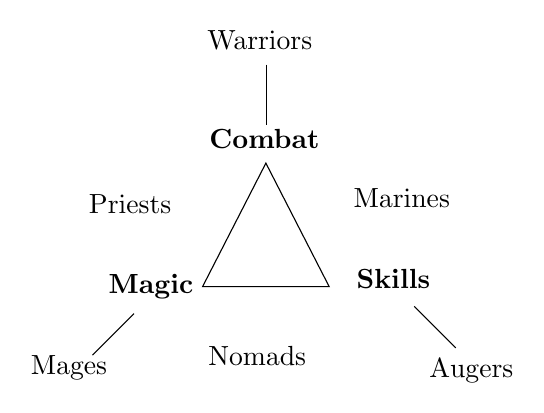
\begin{tikzpicture}[x=0.75pt,y=0.75pt,yscale=-1,xscale=1]
%uncomment if require: \path (0,300); %set diagram left start at 0, and has height of 300

%Straight Lines [id:da5792073549069615] 
\draw    (321.5,53) -- (321.5,82) ;
%Shape: Triangle [id:dp9921269194788708] 
\draw   (321,100.5) -- (351.5,160) -- (290.5,160) -- cycle ;
%Straight Lines [id:da10414083526965556] 
\draw    (257.5,173) -- (237.5,193) ;
%Straight Lines [id:da8045071749370871] 
\draw    (392.5,169.5) -- (412.5,189.5) ;

% Text Node
\draw (291.5,35.5) node [anchor=north west][inner sep=0.75pt]   [align=left] {Warriors};
% Text Node
\draw (234.5,114.5) node [anchor=north west][inner sep=0.75pt]   [align=left] {Priests};
% Text Node
\draw (362,111.5) node [anchor=north west][inner sep=0.75pt]   [align=left] {Marines};
% Text Node
\draw (206.5,192) node [anchor=north west][inner sep=0.75pt]   [align=left] {Mages};
% Text Node
\draw (292,187.5) node [anchor=north west][inner sep=0.75pt]   [align=left] {Nomads};
% Text Node
\draw (398.5,193.5) node [anchor=north west][inner sep=0.75pt]   [align=left] {Augers};
% Text Node
\draw (363.5,150.5) node [anchor=north west][inner sep=0.75pt]   [align=left] {\textbf{Skills}};
% Text Node
\draw (244,153) node [anchor=north west][inner sep=0.75pt]   [align=left] {\textbf{Magic}};
% Text Node
\draw (292.5,83) node [anchor=north west][inner sep=0.75pt]   [align=left] {\textbf{Combat}};


\end{tikzpicture}
\end{center}

The three backgrounds at the ends of the spokes are thus Warrior (for those exclusively trained in combat) Mages (Magic), and Augers (Skills). As for the areas between the spokes, a background that combines Magic and Combat produces the Priest, someone with a knowledge of Magic and the physical training to back it up. Combining Magic and skills yields a Nomad, with training in the mystical arts as well as skills. And finally, mixing Combat and Skills produces a Marine, a person with a need for fighting ability and quick and nimble movements.

\begin{normbox}[Adventurer Background Stats]
\begin{tabular}{@{}l l}
\small
\textbf{Adventurer Background} & \textbf{Most Important Stat}\\
\midrule
\indy{Warrior} & \CSE and \STR\\
\indy{Priest} &  \PWR and \CSE\\
\indy{Magician} &  \PWR and \INT\\
\indy{Nomad} &  \PER and \HEA\\
\indy{Auger} &  \INT and \CSE\\
\indy{Marine} &  \AGI and \STR
\end{tabular}
\end{normbox}

Each background has one or more stats that is very important to the successful practice of the profession, as given in the above table. If your adventurer's highest stat is
STR, they probably would fare best as a Warrior. If they have a high PER, you probably should consider making them a Nomad, etc.\\
You must now choose an available background for your adventurer. Consider not only the stats, but also what you envision your persona becoming, or what you want to roleplay. You are not forced to pick the background that matches the highest stat. In fact, successfully role-playing (for example) an adventurer with a high STR and a mediocre INT as a Auger rather than a Warrior is very rewarding, not to mention entertaining, to you, the GM, and other players.Here are descriptions of the available backgrounds to further help you make a selection:\\
- A \indy{Warrior} relies upon their skill at arms. They are proficient at fighting and confident in their ability to succeed with force. While they might serve in an army, a warrior prefers individual combat and is more likely found employed as a bodyguard, mercenary, constable, or a guard.\\
- A \indy{Priest} is devoted to the service of a deity, forever at that deity's disposal to spread their faith and worship throughout the world. A priest is willing for fight for their deity's cause, but can also use god-given magical powers to further their goals.\\
- A \indy{Magician} is a practitioner of one of four types of elemental magics, using his magics to affect the world and gain wealth, recognition and influence. A magician is often consulted and employed by others to accomplish their goals.
The spells available in each element give a definite flavor to the personality and style of play of a magician. Fire and Air magicians tend to have more offensive spells, whereas Earth and Water mages are more defense oriented. Fire and Earth magic tends to be more individual in nature, while many Air and Water spells are useful to support and maintain a group of adventurers. If your adventurer is going to become a magician, bear these generalities in mind to select the elemental style that matches your adventurer's personality.\\
- Brought up learning to think to solve their problems, an \indy{Auger}'s basic tenet is to live up to their potential, learning to utilize their best skills and making the most of any situation.\\
- Born to the seas, a \indy{Marine} is a member of the traveling armies that plies the seas of Jaern. Ready with a quick story of marine heroes of the past, today's marine attempts to make a name for themselves and their shipmates. They adventure for fame, and are always ready for a good fight and a large tankard of ale.\\
- Members of a tight-knit group of families, \indy{Nomads} mistrust all other Jaernians and rarely travel among them. They are rumored to have various mystical and magical powers, so most people shun them, unsure of their intentions.

After choosing one of these, place it on the adventurer card after "Background." If you're still uncertain, scan the list of Model Adventurers beginning on \tcpage{\pageref{create-models}} for ideas and suggestions. If it appears your adventurer suffers from hopelessly inadequate stats, they would probably not become an adventurer in a fantasy world. Ask the GM; they may allow you to discard this would-be adventurer and start over.
\section{Languages}
You need to know which \indy{languages} (if any) your adventurer speaks to know how they can communicate with actors and other adventurers. Knowledge of languages is an intelligence-based skill, and beginning adventurers may know zero, one or two languages.
\label{create-language}
\begin{normbox}[Learned Language]
\begin{tabular}{l l l}
\small
INT & \makecell{Initial\\\#} & \makecell{Max\\\#}\\
\midrule
3 - 5 & 0 & 0\\
6 - 8 & 1 & 1\\
9 - 11 & 2 & 2\\
12 - 14 & 2 & 3\\
15 - 17 & 2 & 4\\
18 - 20 & 2 & 5\\
21 - 23 & 2 & 6\\
24+ & 2 & 7\\
\end{tabular}
\end{normbox}

Adventurers having an \INT of less than 6 cannot speak coherently. They may know how to say isolated words or phrases, and can generally understand simple sentences. Playing adventurers with a low INT is very challenging because the player must communicate through actions rather than words.

The first language an adventurer with an INT greater than 6 learns is his racial language. This is Paroli for all human adventurers. Half-breed adventurers may pick one of their racial languages as their native tongue or the tongue of whomever raised him, whichever is most appropriate. The first language is always known at a skill rank of 9 or the adventurer's INT, whichever is lower.

With an INT above 8, the player may choose a second language. For non-human adventurers, it would be prudent to pick the common tongue of the area to simplify communications. This second language is initially known at a skill rank of 6.

The available languages are:
\begin{normbox}[Languages]
\begin{tabularx}{\linewidth}{@{} l X }
\small
Breziak & Human tongue\\
Dwarvish & Race tongue of dwarves\\
Elvish & Race tongue of most elves\\
Entish & Spoken by intelligent forest creatures\\
Ferric & Human tongue\\
Geleik & Tongue of the elves of Silvan Isle\\
Haoogh & Speech of the southern pirates\\
Orcish & Race tongue of orcs\\
Paroli & Race tongue for humans and common tongue\\
Sel'ict & Race tongue of the lizard men\\
Trejon & Ancient human tongue\\
\end{tabularx}
\end{normbox}
\setlength{\columnsep}{0.25cm}
\section{Rating}
Your GM must be able to balance your adventuring party against some opponents it might meet. Your adventurer's \indy{Rating} is how many adventurers they have experienced. Set this at two now, and each time he finishes a gaming session, add one. A starting rating of two represents the skills that you choose in creating your adventurer. Your GM may ask for this number from all the players at the beginning of a gaming session.
\section{Date}
At the beginning and end of each adventure, the Game Master will tell you the current game date. The amount of time elapsed between adventures is important for curing damage, doing research, being pregnant, etc. The date is in ISO 8601 format (Year-Month-Day), such as 10080-06-15 SF (Since Founding). Record the current date minus your age on your card as your date of birth (DOB).
\section{Nomadic Prefix Names}
If your adventurer is a nomad, then they must know their own prefix name, or \indy{Epokonom}. Roll \tcdieroll{1d20} and look at the following table. Put this prefix before your adventurer's name.
\vspace{-5pt}
\begin{normbox}[Nomad Prefix Names]
\begin{tabular}{l l|l l}
\small
Roll & Prefix & Roll & Prefix\\
\midrule
1 - 5 & Raz- & 16 & Ald-\\
6 - 9 & Car- & 17 & Edo-\\
10 - 12 & Oka- & 18 & Ijo-\\
13 - 14 & Vem- & 19 & Bez-\\
15 & Lar- & 20 & Sag-\\
\end{tabular}
\end{normbox}
\setlength{\columnsep}{0.25cm}
\section{Name}
Each adventurer must have a name of some sort. Choose a name for your adventurer and place it in the upper left-hand corner of the card. After this put your real name in parenthesis. This will help the Game Master to remember whose adventurer is whose.
\section{Profession}
Your adventurer may have a regular job to bring in a steady income. After your adventurer's skills are selected (see \tcpage{\pageref{create-skills}}), you may choose one as their profession.
\section{Adventurer Models}
Players buy attributes for their adventurers using experience points. Physical equipment is bought with silver pieces. This buying allows you to make your adventurer's abilities fit your perception of her personality.

To simplify making a new adventurer, several different Model Adventurers are reproduced here. If you wish to pick one of these, just copy the information from the chosen model that matches your adventurer's background onto an adventurer card. For each defense value listed in the model, plug in the appropriate stats from your adventurer (dividing them by 5 and rounding down as shown) and add the results to find the your adventurer's defense values. If they are an elf, add one on their MDV for Exceptional PER. If they are an orc, add one to his GDV for Exceptional WIL. Your adventurer is ready to play.

Each model allows you 20\% more attributes than if you had bought all the attributes separately. This extra does not make the adventurer more powerful; it is used to buy attributes that give added flavor and a direction for further development. Once selected, models cannot be modified or changed except to buy new attributes (or upgrade current ones) with earned experience points (see \nameref{create-buying} on \tcpage{\pageref{create-buying}}).

If none of the models fit your idea of your adventurer's personality, and your GM is allowing custom adventurer creation, skip this section and read \nameref{create-buying} to learn how to complete your adventurer's creation.

Each adventurer prototype specifies the values for the following attributes:

\begin{normbox}[Model Attributes]
\noindent\begin{tabularx}{\columnwidth}{@{} l X}
\indy{Damage Points} (\DP) & Relative health\\
\indy{Combat Modifier} (\CM) & Ability using hand-to-hand weapons\\
\indy{Missile Modifier} (\MM) & Ability using bows, slings and crossbows\\
\indy{Grapple Modifier} (\GM) & Ability to grapple\\
Spell type & Declared type of spells (EARTH, FIRE, AIR, WATER, and DIVINE)\\
\indy{Spell Group}s & Ability to use various spell groups\\
\indy{Incants} & Specific nomadic items and talisman\\
\indy[Skill]{Skills} & Purchased skills and their ranks\\
\indy{Combat Defense} (\CDV) & Resistance to being struck\\
\indy{Missile Defense} (\MDV) & Resistance to being hit by missiles\\
\indy{Grapple Defense} (\GDV) & Resistance to being grappled\\
\end{tabularx}
\end{normbox}
\subsection{Models}
\label{create-models}
TBD
\section{Experience Points}
\indy{Experience Points} (\EP) are the currency used to buy such attributes as skills, stats, spells groups, damage points, and melee modifiers. Your adventurer is awarded EP during and after an adventure in several ways, depending on the method chosen by your GM. Using experience points in this way simulates any training or study that might be required to acquire or improve an ability without actually going through the tedium and boredom of doing so during a gaming session. By the way, when an adventure ends, don't forget to add one to the Rating entry on the adventurer's card. Your GM uses the Rating to get a rough idea of how much experience your adventurer has had so that they may balance the difficulty of an adventure against the power of the adventurers.

You may specify that a portion of the awarded experience be set aside and used later to buy attributes. There is no limit to the amount of experience your adventurer may hold, but it makes little sense to hold it longer than needed to buy the attributes sought.
\section{Buying}
\label{create-buying}
If you have not chosen an Adventurer Model, your adventurer is given 5,000 EP with which to buy:
\begin{normbox}[Things You Can Purchase With Experience]
\begin{tabular}{@{}l l}
STATS & STR, INT, etc.\\
DAMAGE POINTS  & Ability to survive injury\\
MELEE MODs & Ability to resist physical damage\\
SPELLS & Magician and Priest magic\\
INCANTS & Nomadic rituals\\
LANGUAGES & Spoken languages\\
ABILITIES & Useful skills and abilities\\
\end{tabular}
\end{normbox}
All buying must be done either when creating an adventurer or between adventures, and must be witnessed by the GM or their representative. The majority of the time this will be done when the adventurer has returned to a civilized setting, where the resources for training are most likely to be found. If an adventure is one in a series, and no game time has passed since the previous adventure, your GM may disallow buying attributes until after the entire sequence of adventures has been completed.

All attributes start at an initial rank of zero and may be bought upward one point at a time. To buy new attributes, or increase the value of an old one, multiply the base cost of the attribute by the point value you wish your adventurer to gain.

\textit{If Marna (a priestess of Osiris) attempts to raise her teaching skill (base cost 100 EP) from 8 to 9, she must expend 100 x 9 or 900 EP to do so.\\
If George the Magnificent (a Warrior) wants to raise his disguise attribute (base cost 50 EP) from 11 to 12, it will cost him 12 x 50 x 3 or 1800 EP. The 3x multiplier is included because the skill is an Auger skill, and George is a Warrior.} 

See \nameref{create-skills} on \tcpage{\pageref{create-skills}} for more information on purchasing skills outside your class.
\subsection{Buying up from zero}
While attributes are usually bought one point at a time, sometimes it is necessary to buy one from zero up to a high value. To do this, we use a little bit of math . . .\\
To buy something from zero to an arbitrary value, call that value N,
\begin{normbox}[Attribute Purchase Equation]
\large
$Total Cost = \frac{N * (N+1)}{2} * Base Cost$
\end{normbox}
For example, to buy damage points (base cost 25 EP) from zero up to 16 would cost as follows:
\begin{normbox}[Attribute Purchase Example]
\large
$\frac{16 * (16+1)}{2} * 25 = \frac{16*17}{2} * 25 = 3,400 EP$
\end{normbox}
If the formula above is too intimidating, use the following table. Cross reference your adventurer's current rank in the attribute against the desired rank, then multiply the number from the table by the base cost of the attribute to find the experience point cost.
\end{multicols*}
\begin{center}
\begin{normbox}[Skill Purchase Multiplier Reference]
\begin{tabular}{@{}l l l l l l l l l l l l l l l l l l l}
\small
\textbf{OLD} & \multicolumn{16}{c}{\textbf{NEW RANK}}\\
\textbf{RANK} & \textbf{1} & \textbf{2} & \textbf{3} & \textbf{4} & \textbf{5} & \textbf{6} & \textbf{7} & \textbf{8} & \textbf{9} & \textbf{10} & \textbf{11} & \textbf{12} & \textbf{13} & \textbf{14} & \textbf{15} & \textbf{16} & \textbf{17} & \textbf{18}\\
0 & 1 & 3 & 6 & 10 & 15 & 21 & 28 & 36 & 45 & 55 & 66 & 78 & 91 & 105 & 120 & 136 & 153 & 171\\
1 & -- & 2 & 5 & 9 & 14 & 20 & 27 & 35 & 44 & 54 & 65 & 77 & 90 & 104 & 119 & 135 & 152 & 170\\
2 & -- & -- & 3 & 7 & 12 & 18 & 25 & 33 & 42 & 52 & 63 & 75 & 88 & 102 & 117 & 133 & 150 & 168\\
3 & -- & -- & -- & 4 & 9 & 15 & 22 & 30 & 39 & 49 & 60 & 72 & 85 & 99 & 114 & 130 & 147 & 165\\
4 & -- & -- & -- & -- & 5 & 11 & 18 & 26 & 35 & 45 & 56 & 68 & 81 & 95 & 110 & 126 & 143 & 161\\
5 & -- & -- & -- & -- & -- & 6 & 13 & 21 & 30 & 40 & 51 & 63 & 76 & 90 & 105 & 121 & 138 & 156\\
6 & -- & -- & -- & -- & -- & -- & 7 & 15 & 24 & 34 & 45 & 57 & 70 & 84 & 99 & 115 & 132 & 150\\
7 & -- & -- & -- & -- & -- & -- & -- & 8 & 17 & 27 & 38 & 50 & 63 & 77 & 92 & 108 & 125 & 143\\
8 & -- & -- & -- & -- & -- & -- & -- & -- & 9 & 19 & 30 & 42 & 55 & 69 & 84 & 100 & 117 & 135\\
9 & -- & -- & -- & -- & -- & -- & -- & -- & -- & 10 & 21 & 33 & 46 & 60 & 75 & 91 & 108 & 126\\
10 & -- & -- & -- & -- & -- & -- & -- & -- & -- & -- & 11 & 23 & 36 & 50 & 65 & 81 & 98 & 116\\
11 & -- & -- & -- & -- & -- & -- & -- & -- & -- & -- & -- & 12 & 25 & 39 & 54 & 70 & 87 & 105\\
12 & -- & -- & -- & -- & -- & -- & -- & -- & -- & -- & -- & -- & 13 & 27 & 42 & 58 & 75 & 93\\
13 & -- & -- & -- & -- & -- & -- & -- & -- & -- & -- & -- & -- & -- & 14 & 29 & 45 & 62 & 80\\
14 & -- & -- & -- & -- & -- & -- & -- & -- & -- & -- & -- & -- & -- & -- & 15 & 31 & 48 & 66\\
15 & -- & -- & -- & -- & -- & -- & -- & -- & -- & -- & -- & -- & -- & -- & -- & 16 & 33 & 51\\
16 & -- & -- & -- & -- & -- & -- & -- & -- & -- & -- & -- & -- & -- & -- & -- & -- & 17 & 35\\
\end{tabular}
\end{normbox}
\end{center}
\begin{multicols*}{2}
\section{Stats}
Of all the attributes, stats are arguably the most important. Stats are the basis for most resistance checks (the avoidance of effects), and determine the maximum value for most other attributes (skills, languages, spell groups, etc.). At a base cost of 500, they are also very expensive to increase. For example, to buy STR from 14 to 15 would cost 500 x 15 = 7,500 experience points.

A physical stat may not be increased more than 4 above the initial roll, to reflect the notion that training and practice can only increase a physical ability so much.
\section{Damage Points}
\textbf{Damage points} (\textbf{DP}) indicate your adventurer's ability to avoid damage during combat. As you buy this total higher, your adventurer becomes more skillful at dodging, moving and twisting to avoid being damaged while fighting. If they are injured, damage points are temporarily subtracted from their total DP; the new total indicates their relative condition.

Lost DP may be regained by resting. A full night's rest (at least eight hours; twelve for those with no soul, like elves) restores a number of DP equal to the adventurer's HEA divided by five (by two for those with the \textbf{Exceptional HEA} attribute, like most dwarves), rounded down. Damage points may not be restored beyond the original maximum DP total.

The base cost for DPs is 25. Your adventurer must have DPs to survive, so here is a chart of the total cost of buying damage points up from zero.

\begin{normbox}[Buying Damage Points]
\begin{tabular}{l l|l l|l l}
DP & Cost & DP & Cost & DP & Cost\\
\midrule
1 & 25 & 8 & 900 & 15 & 3000\\
2 & 75 & 9 & 1125 & 16 & 3400\\
3 & 150 & 10 & 1375 & 17 & 3825\\
4 & 250 & 11 & 1650 & 18 & 4275\\
5 & 375 & 12 & 1950 & 19 & 4750\\
6 & 525 & 13 & 2275 & 20 & 5250\\
7 & 700 & 14 & 2625 & 21 & 5775\\
\end{tabular}
\end{normbox}

Buying damage points with experience actually simulates additional training to avoid being wounded. This could be handled as another defensive modification, but being able to take more damage yields the same effect, is easier to keep track of, balances quite nicely, and is more fun to play.

When buying damage points, you are only increasing your adventurer's maximum DP, not their current DP total. New DPs are only gained after resting, according to the DP recovery rule above.
\section{Melee Modifiers}
Every adventurer has three modifiers, or Mods, that help determine success in combat. The \textbf{Combat Modifier (CM)} is added to all 1d20 "to strike" rolls you make when
your adventurer attacks using a hand-to-hand weapon. The \textbf{Missile Modifier (MM)} is added to all "to hit" rolls from bows, crossbows and thrown objects. The \textbf{Grapple Modifier (GM)} is used when wrestling or boxing an opponent. Mods start at rank zero and are bought upward like any other attribute. The base cost depends on your adventurer's background:

\begin{normbox}[Melee Modifier Costs]
\begin{tabular}{l l l l}
\small
\textbf{Background} & \textbf{Combat} & \textbf{Missile} & \textbf{Grapple}\\
\midrule
Warrior & 200 & 200 & 200\\
Priest & 300 & 300 & 400\\
Mage & 400 & 500 & 600\\
Nomad & 500 & 600 & 500\\
Auger & 400 & 400 & 400\\
Marine & 300 & 400 & 200\\
\end{tabular}
\end{normbox}
\normalsize
Subtract the calculated \textbf{EP} from your adventurer's expendable EP total, then place the values for these on the \textbf{Adventurer Card} after \textbf{Combat}, \textbf{Missile}, and \textbf{Grapple}.
\section{Spells}
There is more to using magic in \textbf{AQ/Jaern} than is given here, but you need to understand experience point costs
and stat limitations to decide whether your adventurer is suited to magic use. Spell casting mechanics are discussed in Chapter \textbf{\nameref{ch:play-adventurer}}, \tcpage{\pageref{ch:play-adventurer}}.\\
\textbf{Spells} are of two varieties: Divine and Elemental. \textbf{Divine magic} is the magic used by priests, granted them by their deities. \textbf{Elemental magic} is used by magicians to harness the raw power of the elements. Both styles of magic
are bought in similar ways.
Adventurers buying elemental magic must declare which one of the four elements (Earth, Fire, Air, or Water) they will use as the source of their power. List this choice on the \textbf{Adventurer Card} under "Element."
If an adventurer wants to purchase priestly magic, he must declare \textbf{allegiance} to a specific deity, who will serve as the source of his magic. This is listed on the card under "Deity" as the primary go or goddess to whom the adventurer owes allegiance.
Spell effects for both elemental and divine magic are divided into groups. The spells in each group are related in some fashion, and are ranked in ascending order of power.
Spells in a group must be acquired in ascending order, as the ability to cast the more powerful spells is built on the knowledge learned from casting the less powerful spells in the group.
Elemental spells are divided into \textbf{core} spells, usable by all magicians, and element-specific spells that may only be used by the appropriate mages.
Priestly \textbf{spell groups} are also divided into two types: \textbf{core} spells that are common to all devout casters, and \textbf{deity-specific} spell groups that manifest the particular sphere of influence of each deity.
The base cost for each spell group varies and is listed in the spell descriptions. Most spell groups have a base cost of 300 EP; one spell group in each element has a base
cost of 600 EP.
\subsection{Acquiring Spells from Other Elements}
Besides their chosen element, adventurers may purchase spells in the element they dominate at double the base cost. They may not purchase spells in any other element.
Dominance is discussed in \textbf{Chapter \ref{ch:play-adventurer}}, but briefly Fire dominates Air, Air dominates Water, Water dominates Earth, and Earth dominates Fire. Thus an earth magician could also learn fire spells, but not air or water spells.
\subsection{Stat Limitations}
Your adventurer's \textbf{INT}, divided by 2 and rounded down, dictates how many elemental spell groups he may buy; \textbf{CSE} is the limiter for divine magic. Thus if your adventurer has an INT of 12 and a CSE of 15, they may not buy into more than 12/2 or 6 elemental spell groups and 15/2=7.5 (round down to 7) divine spell groups.
Your adventurer's \textbf{PWR} stat determines the highest rank that may be bought within any spell group, e.g., someone with a PWR of 13 may not buy above rank 13 in any spell group. Also, your adventurer may not buy a spell group's rank higher than it has listed spells.
\subsection{Buying of Spells by Other Backgrounds}
Normally only magician or priest adventurers buy spells, but those in other backgrounds may desire at some point in their careers to dabble in magic. Like any magician or priest they must choose an element and/or declare devotion to a deity. Spell groups are purchased at \textbf{triple} the base cost; buying into the subservient element costs \textbf{sextuple} the base cost.

\begin{normbox}[Spell Cost Multiplier]
\begin{tabular}{l l l l l l}
\small
\textbf{Buyer} & \textbf{Earth}  & \textbf{Fire} & \textbf{Air} & \textbf{Water}  & \textbf{Divine}\\
\midrule
Earth & 1 & 2 & - & - & 3\\
Fire & - & 1 & 2 & - & 3\\
Air & - & - & 1 & 2 & 3\\
Water & 2 & - & - & 1 & 3\\
Div/Earth & 3 & 6 & - & - & 1\\
Div/Fire & - & 3 & 6 & - & 1\\
Div/Air & - & - & 3 & 6 & 1\\
Div/Water & 6 & - & - & 3 & 1\\
NM*/Earth & 3 & 6 & - & - & 3\\
NM*/Fire & - & 3 & 6 & - & 3\\
NM*/Air & - & - & 3 & 6 & 3\\
NM*/Water & 6 & - & - & 3 & 3\\
\end{tabular}
\end{normbox}
\normalsize
*This also applies to a non-magician who picks up divine magic and then elemental magic as well.

\section{Incants}
\textbf{Incants} are rituals performed by by nomads. These
incants take the form of Alchemical mixtures, Songs, Talisman, Imprints (tattoos), and Spiritual Invocations. The ability to perform the ritual is purchased by the nomad by
rank and at stated base cots. When the ritual is performed, many require a proper ingredient. An incant can not be purchased at a rank higher than half the adventurer's \textbf{PER} stat, rounded down.
\subsection{Preparing Incants by Other Backgrounds}
If an adventurer from another background wishes to delve into the arcane, they must seek out a nomadic \textbf{rondo}, renounce their allegiance to any gods, and be accepted by the nomads. They must be inducted into their ranks before they can learn any spiritual magic. They undergo \textbf{The Seraei} to find and bind with a \textbf{Guardian Spirit}. Even then, they must pay \textbf{triple} the normal experience cost since they have not yet learned the stories, songs an traditions of those brought up within the rondo.
\section{Languages}
The key to increasing your adventurer's ability in a language is to find someone with a rank in that language at least four higher than the rank your adventurer wishes to obtain. He may buy the language skill to the desired rank at a base cost of 100 EP, besides the teacher's fee (monetary or service), if any. Remember that your adventurer's \textbf{INT} limits the number of languages they may learn (see \tcpage{\pageref{create-language}}). Furthermore, the rank of a language may never exceed the
INT value. Language rank definitions are as follows:

\begin{normbox}[Language Rank Definitions]
\begin{tabular}{p{0.085\linewidth} p{0.7\linewidth}}
1-2  & Knows individual words, no sentences\\
3-4  & Can speak common phrases\\
5-6  & Can be understood, but speaks w/accent\\
7-8  & Can hold conversations, read, and write\\
9-10  & Speaks like a native\\
11-15  & Can speak persuasively as an entertainer or politician\\
16+ & Can use speech as a weapon as a poet or bard\\
\end{tabular}
\end{normbox}
\section{Skills}
\begin{multicols*}{2}
Skills allow your adventurer to be more than their basic background permits. Each skill has a rank starting at one and going upward. An adventurer possessing a skill at rank 1 is complete novice at that skill, while holding a rank 18 shows an almost godlike command of the craft.
\begin{normbox}[Skill Rank Definitions]
\begin{tabular}{l l}
1 - 2 & Beginner\\
3 - 4 & Novice\\
5 - 6 & Apprentice\\
7 - 8 & Journeyman\\
9 -10 & Professional\\
11-12 & Craftsman\\
13-15 & Master\\
16+ & Guild-master\\
\end{tabular}
\end{normbox}
\end{multicols*}
\subsection{Learning Skills}
Skills may be taught by an actor, or by one adventurer to another. The teacher must rank at least four higher than the student's desired rank; the minimum learning time is one week times the skill rank the student is attempting to learn. The student must spend the required EP, plus a teacher's fee (monetary or service), if any.
Each skill's \textbf{associated stat} governs the maximum rank your adventurer may purchase, e.g., INT based skills may not be bought higher than your adventurer's INT rank.
On the next page is a listing of available skills. Those listed as "res" cannot be bought without consulting the GM. All the others can be bought by a beginning adventurer. The number listed in the "Extra Dice" column is the number of extra dice used to \textbf{default} that skill. Skills labeled with "non" cannot be defaulted. Full descriptions of each skill are in \textbf{Chapter \nameref{ch:skills}} beginning on \tcpage{\pageref{ch:skills}}.
\label{create-skills}
\begin{tcbraster}[raster columns=1,boxrule=0pt,title=\textbf{Skills},left=0pt,right=0pt,top=0pt,bottom=0pt,boxsep=0pt,boxrule=0.6pt,lefttitle=2.5mm,toptitle=1mm,bottomtitle=1mm,colbacktitle=Navy,colback=white]
\tcbincludepdf{create-skills.pdf}
\end{tcbraster}
\section{Money}
Each adventurer has a small initial supply of silver pieces to spend on equipment. If you did not pick an adventurer model, roll \tcdieroll{3d6} and multiply the total by 10 to determine your adventurer's starting money.
\section{Equipment}
Silver is used to buy adventuring equipment. Items on the following table may be bought or sold when in a town and between adventures, without consulting the GM. Equipment may be sold back to the merchants in town for one half of the listed price. Place any equipment bought under "Equipment" on the \textbf{Adventurer Card} and subtract the proper amount of silver.

All prices are in silver. The exchange rate is 100 copper coins = 10 silver coins = 1 gold coin. Any item that is iron or steel may be silvered by quadrupling the cost. Items may also be made of other materials, if feasible.

\begin{normbox}[Material cost multiplier chart]
\begin{tabular}{@{}l l}
Wood  & 1/2 Cost\\
Iron  & Base Cost\\
Silver Plated  & 4 Times\\
Solid Silver  & 10 Times\\
Gold Plated  & 16 Times\\
Platinum Plated  & 64 Times\\
Solid Gold  & 100 Times\\
Steel  & 200 Times\\
Solid Platinum  & 1,000 Times\\
Solid Adamantite  & 2,000 Times\\
\end{tabular}
\end{normbox}
\end{multicols*}
\setlength{\columnsep}{0cm}
\begin{multicols*}{4}
\begin{tcbraster}[raster columns=1,boxrule=0pt,title=\textbf{Equipment},left=2pt,right=0pt,top=0pt,bottom=0pt,boxsep=0pt,boxrule=0.6pt,lefttitle=2.5mm,toptitle=1mm,bottomtitle=1mm,colbacktitle=Navy,colback=white]
\tcbincludepdf{create-equipment.pdf}
\end{tcbraster}
\end{multicols*}
\setlength{\columnsep}{\defcolwidth}
\begin{multicols*}{2}
\section{Defense Values}
Once your adventurer is equipped, you can calculate the three defense values, which determine how difficult it is to wound your adventurer in combat. There is a separate defense value for each type of melee: using hand-to-hand weapons (to strike), missiles (to hit), and grappling (to grapple). Add up the factors for each defensive component to calculate your adventurer's three defense values. They only need to be recalculated if any of the component values change.
If the adventurer is bound or unconscious, skip the sections on Mobility, Agility, and Stat Modifiers. Set your adventurer's defense values at zero and start at the section on Armor.
\subsection{Mobility}
If your adventurer is standing and alert, they start each defense value with 3.
\subsection{Agility}
If your adventurer is alert and able to move, add 1 point to each defense value for each 5 points of AGI (rounded down) that your adventurer has. Add an additional one point to each defense value if your adventurer has \textbf{Exceptional AGI} (That is if they are a lizard).
\subsection{Stat Modifiers}
Each defense value is dependent on one additional stat. Take the related stat for each defense value, divide it by five and round down. Add this to the appropriate defense value.
\begin{normbox}[Melee Defense Stats]
\begin{tabular}{@{}l l l}
Combat & (CDV) & STR\\
Missile & (MDV) & PER\\
Grapple & (GDV) & WIL\\
\end{tabular}
\end{normbox}
Elves gain an additional one on their MDB for \textbf{Exceptional PER} and orcs one on their GDV for \textbf{Exceptional WIL}.
\subsection{Armor}
Different types of armor increase your adventurer's defense. Armor also determines how fast he can move each round during combat. Look up the type of armor they are wearing on the following table and add the modifier to each defense value:
\begin{normbox}[Armor Defense and Movement]
\begin{tabular}{@{}l p{0.125\linewidth} p{0.125\linewidth} p{0.125\linewidth} p{0.125\linewidth}}
\small
\textbf{Armor} & \textbf{Combat} & \textbf{Missile} & \textbf{Grapple} & \textbf{Move}\\
\midrule
Naked & 0 & 0 & 0 & 60'\\
Clothed & 1 & 1 & 1 & 50'\\
Leather & 2 & 2 & 2 & 40'\\
Chain Mail & 4 & 1 & 2 & 30'\\
Steel Chain Mail  & 5 & 2 & 2 & 30'\\
Plate Mail & 6 & 4 & 2 & 20'\\
Steel Plate & 8 & 5 & 2 & 20'\\
\end{tabular}
\end{normbox}
\subsection{Defensive Devices}
Different kinds of shielding devices affect defense values. Of course, they must be worn or properly used to be effective.
\begin{normbox}[Device Defensive Additions]
\begin{tabular}{l l l l}
Device & Combat & Missile & Grapple\\
Buckler & 1 & 0 & 0\\
Helmet & 1 & 1 & 0\\
Shield & 3 & 3 & 1\\
Steel Shield & 4 & 3 & 1\\
\end{tabular}
\end{normbox}
\subsection{Weapons}
Many weapons may be used defensively as well as offensively. If your adventurer is currently using such a weapon, look up its defense value adjustment on the \textbf{Weapon Information Table} chart on \tcpage{\pageref{playing-weapon-table}} and add it to your \textbf{CDV} and your \textbf{GDV}.
\end{multicols*}
\chapter{Playing an Adventurer}
\label{ch:play-adventurer}
\index{adventurer!playing}
\setlength{\columnsep}{\defcolwidth}
\begin{multicols}{2}
An \aq game session revolves about the interaction between you, other players, actors, and your \indy{Game Master} as events unfold during play. This chapter presents the rules you and the GM need for a smooth running game. Once learned, you'll find them so simple and natural that they fade into the background, allowing everyone to immerse themselves in the excitement of the adventure without being distracted by constantly consulting tables and charts.
%\vspace{5pt}
\section{Your job as a player}
You must bear one thought in mind when playing Adventure Quest: your GM has gone to much effort to learn and adjudicate the adventure. All their decisions are \ul{final} and
should not be challenged during the game. If you believe that the GM may have made a mistake, or you are uncertain if an event or condition that affects a character was considered (e.g. a spell effect, character trait, or pre-established event), you can ask if that was considered. No GM is infallable, and running an adventure often requires spinning many plates.

If you disagree with any of their decisions, take the GM aside \textbf{after} the game and talk it over. They may have acted on information you don't know, or slightly changed some rules to make the game  different, more exciting, or less predictable. Your GM is under no obligation to explain any result, as the explanation could reveal information that your adventurer should not have.
\section{Use of Dice}
\indx{dice,rolling}
\indx{d4}\indx{d6}\indx{d8}\indx{d10}\indx{d12}\indx{d20}\indx{d30}\indx{d100}
Dice with different numbers of sides are required to play AQ. At a minimum you'll need a \tcdieroll{d4}, a \tcdieroll{d6}, a \tcdieroll{d8}, a \tcdieroll{d12}, and a \tcdieroll{d20}. A \tcdieroll{d10} is available, but a \tcdieroll{d20} can be used in its
place. Percentile rolls (\tcdieroll{d100}) can be rolled with \tcdieroll{2d10} \tcdieroll{2d20}; one die represents the tens digit and the other the ones digit. A \tcdieroll{d100} and a \tcdieroll{d30} are commercially available, but they are not needed to play AQ. Since it is quicker to roll three dice at once rather
than the same die three times, expand your dice collection as needed. Adopting these simple conventions will prevent confusion and misunderstandings about dice rolls:

\begin{enumerate}
\item Make sure someone witnesses all rolls.
\item Don't roll dice until the GM asks you.
\item If any dice fall off the rolling surface, reroll them all.
\item For percentage rolls, the darker die is always the ten's digit. If uncertain, verbally name the ten's die before rolling.
\end{enumerate}
\section{Playing Modes}
\indx{playing!mode}\indx{mode!playing}
Play occurs in one of three \textbf{modes}, which are mainly defined by their time-keeping requirements during play.
\subsection{Summarized Actions Mode}
\indx{playing!summarized actions}\indx{mode!summarized actions}When adventurers must perform a series of mundane actions that are not pertinent to the plot or  enjoyment of the adventure, the GM may simply state these things are occurring, thus briefly summarizing a long time passage. 

If a player feels it's important to clarify an action during this time, he should notify the GM to switch to \indy{Free Action Mode}.

\example{Having conquered the evil Jhelonian prince and rescued the fair Felicia from his clutches, you and your companions procure passage back to your home city of Rougtero. Four uneventful days at sea do not prepare you for the large celebration that takes place when you step foot on the docks.}
\subsection{Free Actions Mode}
\indx{mode!free actions}\indx{playing!free action}
For most of an adventure session you will play in near real time. The GM freely accepts actions stated by the players and gives the results of those actions. This mode of play is suspended only when the GM decides to summarize a long time period or when melee is initiated.
\subsection{Melee Actions Mode}
\indx{mode!melee actions}\indx{playing!melee actions}
When adventurers, creatures and actors come into conflict with each other, the GM places the game into melee mode. Time is broken down into 4 second combat rounds. Each round, the GM hands out information about the \indy[combat|see{melee}]{combat}, asks for adventurer actions, and reports the results. This cycle is repeated until the melee ends, at which point the GM switches to \indy{Free Action Mode}.

Differing from other systems in which every player participating in a combat rolls to determine their place in the order of initiative, melee in \aq utilizes groupings of melee, in which local, allied participants are grouped together and all of their actions occur simultaneously.
\section{Encounters and Combat}
\label{encounter}\indx{encounter}
When adventurers encounter an actor, a group of actors, or creatures, combat may be the only alternative. The GM accepts and resolves \indy{melee} actions as follows:
\subsection{Distance}
\indx{melee!distance}
When the opportunity exists for adventurers to encounter other creatures or actors, your GM will determine at what distance you are from them. Your adventurer must have \indy{Line of Sight}, \textit{i.e. an unobstructed viewing path}, to see their opponents. Indoors or underground this generally means they must be in the same room or corridor. Outdoors, the prevailing light conditions, the type of plant life, and the general terrain are all factors that the GM must considered.
\subsection{Order of Melee}
\indx{melee!order}
A \indy{Round} is an exchange of blows between two or more opponents. A round lasts \measure{4 seconds} (15 rounds per minute) and is the time unit of combat. The following \indy{Order of Actions} imposes order on an inherently chaotic situation:
\begin{enumerate}
\item Determine \indx{melee!initiative}\indy{initiative}.
\item Each group, in order of initiative, gets an \indx{melee!action phase}\indy{Action Phase}.
\begin{enumerate}
\item \indy[melee!informational questions]{Informational questions}
\item \indy[melee!action preparation]{Action preparation}
\item \indy[melee!actions]{Statement of actions}
\item \indy[melee!results]{Results of actions}
\end{enumerate}
\item \indy[melee!outcome]{Outcome Phase}
\end{enumerate}
\subsubsection{Initiative}
\indy{Initiative} indicates the order in which each side plans and performs its actions. A representative from each group rolls \tcdieroll{2d6} and the results determine the order, highest to lowest, in which actions are taken. There is no simultaneous combat. If players are involved in one group, they win ties. Otherwise if a tie results, each side must roll again until one wins.

For each \indy{Round} a side does not win initiative, it gets to add a cumulative \result{+1} to its roll for each succeeding roll. When a side wins initiative, it gets no such bonus the next round. The GM will likely make use of counters or markers to denote the bonus given to each side of a melee.

There may be more than two groups in initiative, in which case the rounds occur in descending order of initiative. Additionally, groups may merge or split during combat. \example{e.g. a character is revealed to be an impostor or attacks an innocent bystander.} Any changes to initiative groups take effect on the next round. 
\subsubsection{Informational Questions}\indx{melee!informational questions}
The GM starts the adventurers' action phase by taking questions from the players about the current situation and answering them according to the adventurers' knowledge at the time. Players may talk with each other about the situation, about playing style and rules questions, but \uline{MAY NOT} tell each other what they plan to do or exchange information between adventurers. When all questions have been answered, the GM continues.
\subsubsection{Action Preparation}\indx{melee!action preparation}
The GM asks all players to prepare actions. Each player must decide what one action their adventurer will do during the upcoming round. Players \uline{MAY NOT} talk with each other during this time. If play becomes very intense or important, the GM may ask for actions in writing. When all actions are ready, play continues.
\subsubsection{Statement of Actions}\indx{melee!actions}
One at a time, the GM asks each player what their adventurer's action is for the round. Since these actions are occurring simultaneously, the order of the call is unimportant. As each action is revealed, the GM asks the player to make any needed rolls. The player should roll the requested dice and announce the results (including any modifiers). The GM records any results during this phase.
\subsubsection{Results of Actions}\indx{melee!results}
After all actions have been stated and resolved, the GM announces the results of the Action Phase. This includes creatures or people falling to the ground, incidental movement, noise, or visions. The players may ask questions here if the results are unclear. \quip{Remember, sometimes this is intentional and the GM may refuse to answer!}
\subsubsection{Outcome Phase}\indx{melee!outcome}
After all combatants have had their Action Phase, the GM also announces the outcome of any occurrences that are not the direct result of adventurers, actors, or creatures involved in the combat. This includes things like large falling objects, timed explosions, natural disasters, collapsing buildings and disintegrating planets.
\subsection{Surprise}\indx{melee!surprise}
When two groups of adventures, actors or creatures first meet, one group may not notice the other immediately. If this is true, and the non-surprised group attempts a combat
action, the GM will change to Free Action mode allow them a Free Round to perform actions. The GM will continue to allow the Free Rounds until the other party notices their presence. Then the GM will start normal combat.
\section{Actions}
Of course, there are many different actions an adventurer may take during a round, but usually they fall into a few different classes. Each of these is described below to give you an idea of what your adventurer may do during melee.
\subsection{Movement}\indx{melee!movement}
\begin{wrapfigure}[8]{l}[0pt]{115pt}
\begin{normbox}[Armor Restrictions]
\small
\begin{tabular}{@{}l l}
\textbf{Armor} & \textbf{Move Rate}\\
\midrule
Naked & 60'\\
Clothed & 50'\\
Leather armor & 40'\\
Chain armor & 30'\\
Plate mail & 20'\\
\end{tabular}
\end{normbox}
\end{wrapfigure}

It is often necessary to maneuver during combat. Each adventurer has a \indy{Movement Rate} that is the distance they may move in a round when not in direct melee. This distance may be modified by your GM according to terrain, obstacles, or circumstances. If you wish to make any attacks or cast spells, you can only move \result{1/4} your movement rate that round. You can ready weapons, talk, observe the situation or ready actions while moving.

\subsection{Striking}\indx{melee!striking}\indx{striking}
When two opponents are within \measure{5 feet} of each other, they are normally considered \indy[melee!in melee]{in melee}, trading attacks with intent to harm. To determine if a hand-to-hand attack is successful, the attacker rolls \tcdieroll{1d20}, adds their \indy{Combat Modifier} (\CM), plus any other appropriate bonuses, to the result, and compares the total to the \indy{Combat Defense Value} (\CDV) of the opponent. The total must equal or exceed the opponent's CDV to hit.

\example{Valken the Warrior attacks a poor, helpless villager with his once enchanted (+1) long sword. Valken's player rolls a 10 on 1d20. Valken's CM is 1, and the magical sword has a bonus of 1, for a total of 10+1+1 = 12. The poor villager is lying supine on the ground (with Valken's foot on his stomach), so it has a CDV of 5.}

\example{Valken's player announces he has struck CDV 12. Since 12 is greater than 5, Valken strikes the orc with his long sword. The GM tells Valken's player that he has struck and directs him to roll damage. The player rolls 1d10 (for long sword damage), getting a 5. He adds 1 (for the magic sword) and announces that Valken has done 6 points of damage. At the end of the round, since the poor villager only started with 4 DP, the GM announces the he is slain.}
\subsubsection{Impaling}\indx{melee!impaling}\indx{weapon!impaling}
\indy{Impaling} our opponent with your weapon is a style of attack that uses the same attack roll and defense value as striking, but can cause considerably more damage. Charging an opponent with a set weapon or setting a weapon and allowing an opponent to run themselves through are both examples of impaling. Impaling is only effective when the target or the impaler have been moving at their \tcdefine{maximum movement rate for at least one full round} and the other is stationary or moving closer. Impaling is accomplished with  standard roll to strike, but modifiers and skills are not applicable.
\subsection{Hitting}\indx{melee!hitting}
Missile weapons are used very much like hand-to-hand weapons, except you use the attacker's \indy{Missile Modifier} (\MM) and the defender's \indy{Missile Defense Value} (\MDV). If the attacker's \tcdieroll{1d20} roll plus their \MM, plus other bonuses equal or exceeds the defender's \MDV, they have hit and the player rolls \indy{missile damage}.
\subsection{Critical Hits and Misses}\indx{melee!critical hits}\indx{critical hits}
When your adventurer is attempting to attack in any way, examine the result of the attack roll before any bonuses or mods are added. If the die roll is \tcdefine{a 1}, it is an \indx{melee!automatic miss}\indy{automatic miss}, no hit happens, no grapple succeeds, no damage is
done. If the die roll is \tcdefine{a 20}, it is considered a \indx{melee!critical hit}\indy{Critical Hit}. The GM will ask you to roll percentiles (\tcdieroll{2d10} with one die specified as the tens' digit and one die as the ones' digit) to determine its severity. You can cross reference the appropriate table for your attack type in \textbf{Appendix \ref{ap:important-tables} on \tcpage{critical-hits}}
\subsection{Grappling}\indx{melee!grappling}
Whenever an adventurer is within melee range of an opponent, they may attempt to \indy{grapple} rather than strike at the opponent with a weapon. The adventurer must drop anything they are holding at the beginning of the round so that both hands are free. \indy{Shields} take a full round to drop, your adventurer's arm is in a couple of straps.

The player states which grappling option will be used (hold or throw), then rolls \tcdieroll{1d20} and adds the adventurer's \indy{Grapple Modifier} (\GM). If the total is equal to or greater than the opponent's \indy{Grapple Defense Value} (\GDV), the grapple option succeeds, the defender is held, or thrown. If the grapple fails the attacker and defender are still grappling, and must wait until the next round for another attempt.

All this happens during the attacker's portion of the round, so the defender may become the attacker in his portion of the round. Once an adventurer is grappling he may not withdraw unless he is not held, and has the initiative.
\subsubsection{Hold}\indx{melee!hold}
The only action a held person may take is to attempt to break the \indy{hold}. During their round, the held combatant may make a \tcdieroll{4d6} check vs. \STR. Each additional person holding the combatant adds \tcdieroll{1d6} to this \STR check. If the check succeeds, they has broken the attacker's grasp and may take other actions in their latter rounds. If it fails, every subsequent attempt is made adding \result{an additional die} to the \STR check.
\subsubsection{Throw}\indx{melee!throw}
When a \indy{throw} attempt succeeds, the thrower may determine the direction of the throw. However, the distance thrown and what, if any, damage or other results occur must be adjudicated by the GM at the time of the throw.
\subsection{Withdrawal from Melee and Grappling}\indx{melee!withdrawal}
To successfully \indy{withdraw} from melee, the adventurer must not be held when it is his round to take an action. It will take one round to get up from the ground, so their opponent may have further opportunities to grapple before they can escape. Even if an adventurer has got up and run from a grapple, their opponent is free to chase and tackle them.
\subsection{Multiple Combatants}\indx{melee!multiple combatants}
Situations occur where more than one person wants to strike or grapple the same target. If the target and the attackers are relatively the same size, no more than \tcdefine{4 combatants} may attack the same target. A standing target backed up against a wall may only be attacked by \tcdefine{2 combatants}; if in a doorway or tight corridor, only \tcdefine{1 combatant}. If more than the allowed number attempt to attack a single target, all attackers must make a check of \tcdieroll{3d6}, plus \tcdieroll{1d6} for each extra attacker, vs. their \AGI or trip and fall to the floor, losing their attack that round.

A possible exception to this might arise if adventurers behind the attackers want to thrust polearms or spears at the target between the attackers. This might be perfectly feasible; it is up the GM to decide based on the circumstances.
\subsection{Shooting into Melee}\indx{melee!shooting into}\indx{shooting}
Shooting a missile weapon at an opponent who is in melee with adventurers from your party is a dangerous and possibly fatal action. If you attempt to hit an opponent in
melee, and miss, the GM will determine if any others in the combat are potential targets. If so, they will ask you to roll to hit the alternate target, damaging them if you succeed. \quip{Shooting your friends in the back is a good way to earn a quick and violent death.}
\subsection{Other Common Actions}\indx{melee!common action}
It is impossible to list all the actions that might occur during an Action Phase. During play, the GM must adjudicate any unusual actions and assign duration for them. Some common actions and their duration in rounds are given below:
\begin{normboxc}[Common Action Duration]
\indx{melee!action durations}
\small
\begin{tabular}{@{}l c}
\textbf{Action} & \textbf{Duration}\\
Climb 10' of rope & 2\\
Dropping a shield & 1\\
Finding something in backpack & 1-4\\
Getting up from the ground & 1\\
Lighting a torch & 2-10\\
Mount a horse or dolphin & 2\\
Readying weapon & 1\\
Remove chain armor & 4\\
Remove leather armor & 2\\
Remove plate armor & 8\\
Removing backpack & 1\\
Searching a body & 5-20\\
Survey a situation & 1\\
Switching weapons & 1\\
\end{tabular}
\end{normboxc}
\section{Using Skills}
When your adventurer must perform a specific task during play, success or failure is determined by a \indy{skill} check or a stat check. Having an applicable skill gives them a better chance of succeeding, and the higher the skill value, the greater the chance for success.

To check skill use, your Game Master will ask you to roll some \tcdieroll{d6}. If you roll \textbf{your adventurer's skill value or less}, they have successfully applied that skill.

Simple tasks require a roll equal to or below your adventurer's skill value on \tcdieroll{1d6}; moderately difficult tasks require a roll of \tcdieroll{2d6}, and very difficult tasks \tcdieroll{3d6} or more. Remember, your GM is the final authority on needed rolls and can and will apply appropriate modifiers.
\section{Defaulting a skill}
If your adventurer attempts to use a skill they don't have, or fails at an acquired skill, they may still try, but the check is against that skill's associated stat, this is called \indx{skill!defaulting}\indy{defaulting}. The total number of \tcdieroll{d6} to be rolled is that given by the GM, plus the number of dice shown as extra dice for that skill. Restricted skills are so complex that aside from the fact that they must be purchased from the GM, they also may not be attempted by those who have not been taught the skill. Also some skills are based on acquired knowledge, and can not be defaulted. An entry of \tcdefine{reserved} or \tcdefine{N/A} in the extra dice column indicates that skill can not be defaulted.

\example{Alene has bought mountain climbing up to rank 8, and has an AGI of 15. While adventuring she must climb a steep rock face. The rock is damp from rain and somewhat
slippery, so the GM asks Alene's player to roll 8 or less on 2d6. The player rolls a 7, so the skill check succeeds.}

\example{Let's say the player rolled a 10, meaning the skill check failed. The GM allows another chance, using mountain climbing's associated stat (AGI). The player must roll Alene's AGI or less on 4d6 (the 2 dictated by the GM, plus 2 from the extra dice column opposite mountain climbing). The result is a 12, meaning success this time.}
\section{Resistance Checks}
\indy{Resistance Checks} (or \RC) are a measure of your adventurer's resistance to physical and spell effects. When you are subject to such an effect, your GM will state what the effect is, which stat to check against, and how strong the effect is by announcing how many dice you need to roll to resist that effect. Roll that many dice, and if you roll \tcdefine{equal to or lower than your \indy{rank}} in the appropriate stat, you succeed the resistance check and the effect is weakened or negated.
\subsection{Armor Effects of Resistance Checks}\indx{armor}\indx{resistance check!armor}
Different types of armor can diminish your ability to resist certain magical and physical effects. Leather armor restricts mobility, automatically adding \tcdieroll{1d6} to any \textbf{RC (Resistance Check)} against \AGI. Chain mail has, in addition, a large mass of metal that attracts magical energies. An adventurer in chain must add \tcdieroll{1d6} to any RC against \AGI and \PWR. A set of plate mail is extremely heavy and takes considerable strength to wear. An adventurer in plate mail must add \tcdieroll{1d6} to any RC against \AGI, \PWR, or \STR.
\begin{normboxc}[Armor Stat Effects]
\small
\begin{tabular}{@{} l l l}
\textbf{Armor} & \textbf{Stat} & \textbf{Change}\\
\midrule
Leather & \AGI & \tcdieroll{1d6}\\
Chain Mail & \AGI, \PWR & \tcdieroll{1d6}\\
Plate Mail & \AGI, \PWR, \STR & \tcdieroll{1d6}\\
\end{tabular}
\end{normboxc}
\section{Dying and Falling Unconscious}\indx{dying}
If you fight you just might get hurt! When an adventurer is damaged they must temporarily subtract that number of damage points from their damage point total. If the total goes \tcdefine{below 0 DP}, the adventurer \indy[death]{dies} \tcdefine{immediately}. (Since all actions are simultaneous in an action phase, a cure in the same round may prevent the total from going below zero).

If an adventurer's \DP total is between \tcdefine{0 and 5}, the player must roll their adventurer's current \DP total (after damage) or less on \tcdieroll{1d6} to remain conscious. If they fail this roll, the adventurer immediately falls \indy{unconscious}. When (and if) an unconscious adventurer recovers damage points through natural or magical healing, they may reroll to wake up. (This is automatic once \tcdefine{6 DP} is reached).
\section{Stressing Stats}\indx{statistics!stressing}
If desired, adventurers can push themselves beyond the normal limits of their stats by \indx{statistics!stressing}\indy{stressing}. This means that one point of the stressed stat is expended \tcdefine{permanently} to gain some effect. A single stat may not be stressed more than once in a melee, and two stats may not be stressed at the same time. Stressing may be done in any playing mode, but occurs most often during melee and doesn't count as an action. Though the stressed stat can never recover naturally, it can be bought back to its previous rank, or beyond, by spending experience points.

Stressing can not be used for any \indy[skill!check]{skill checks}. Even though \indy{defaulted} skills are rolled against a stat, this is not considered a stat check for the sake of stressing. A defaulted skill roll is a skill attempted without the proper training or knowledge, so no amount of stressing will improve your adventurer's chance of success.

To stress a stat, state to the GM at the \tcdefine{beginning} of your action which stat your adventurer is stressing. Some stats may be stressed in response to the GM asking for an RC. This table summarizes the results of stressing.
\small
\begin{normboxc}[Effects of Stressing]
\small
\begin{tabular}{@{}llll}
\textbf{Stat} & \textbf{\makecell[l]{Resist Bonus}} & \textbf{\makecell[l]{Spell Units}} & \textbf{\makecell[l]{Other  Effects}}\\
\midrule
\makecell[lt]{STR} & \makecell[lt]{2d6} &  & \makecell[lt]{+10 Strike\\+10 Damage}\\
\midrule
\makecell[lt]{INT} & \makecell[lt]{2d6} &  & \\
\midrule
\makecell[lt]{PER} & \makecell[lt]{2d6} &  & \\
\midrule
\makecell[lt]{CSE} &  &  & \makecell[lt]{1 Extra\\\indx{divine!intervention}DI die}\\
\midrule
\makecell[lt]{HEA} & \makecell[lt]{2d6} & \makecell[lt]{+2 rank/\\incant} & \makecell[lt]{Stay\\conscious}\\
\midrule
\makecell[lt]{AGI} & \makecell[lt]{2d6} &  & \\
\midrule
\makecell[lt]{PWR} & \makecell[lt]{2d6} & \makecell[lt]{4 EU \\or 4 DU} & \\
\midrule
\makecell[lt]{COM} &  &  & \\
\midrule
\makecell[lt]{WIL} & \makecell[lt]{2d6} &  & \\
\end{tabular}
\end{normboxc}\\
\normalsize A few of the entries in this table deserve some more explanation.
\subsection{Strength}\indx{stressing!strength}
Stressing \STR during a combat round means your adventurer is making a heroic effort against their opponent. They gain a \tcdefine{+10 modifier} to their "to strike" roll and, if they strike successfully, inflicts an additional \tcdefine{10 DP} on their target.
\subsection{Common Sense}\indx{stressing!common sense}
When a priest feels deserted by their deity during desperate times, they may elect to set common sense aside and put their faith in being delivered from their predicament by their god. Stressing a point of \CSE gives them \tcdefine{1 extra die} when calling forth intervention from their deity. No other background gains this ability.
\subsection{Power}\indx{stressing!power}
Caught in a deadly situation, a caster may stress one point of \PWR to regain \tcdefine{4 lost units}, which must be used in the same round of the stress. These units can be \indy{elemental} or \indy{divine} units.
\subsection{Health}\indx{stressing!health}
When near death, the slightest damage can cause your adventurer to black out, leaving them at their opponent's mercy. By an enormous effort of will, they can stay conscious, but this places their body and health at great risk. Stressing one point of \HEA allows the adventurer to automatically succeed one unconsciousness check.

\indy[nomad]{Nomads} may stress one point of \HEA to add \tcdefine{2 ranks} to any one incant which they are preparing. They can only do this once per day.
\subsection{Comeliness}\indx{stressing!comeliness}
Unfortunately, physical attractiveness is not something that can be improved in times of stress. If anything, the opposite is likely to occur. Stressing your adventurer's \COM doesn't result in any perceptible boon, and may actually make the adventurer seem more frantic to his companions.
\section{Weapons and Their Effects}\indx{weapon!effects}
Adventurers may employ many different weapons in combat. Each weapon is unique in the amount of damage it can do and who may use it.
\indy[weapon!type]{Weapon Type} is the broad classification of each
weapon as Edged, Pointed, Blunt, or Defensive. If a critical hit is rolled, these tell you which Critical Hit Table to consult. No criticals are possible with a defensive device.

"STR" is the minimum \STR value required to effectively use the weapon. The "DV" column is the \indy{Defensive Value} (\DV) adjustment for that particular weapon; this value is added to the adventurer's \CDV and \GDV when that weapon is in use. Note that \indy[weapon!one-handed]{one-handed weapons} are worth \tcdefine{1 DV}, \indy[weapon!two-handed]{two-handed weapons} are worth \tcdefine{2 DV}, and most defensive weapons are worth \tcdefine{3 DV}. Two-handed weapons (those listed with a DV of two) must be used two-handed.

\indx{weapon!damage}The value in the \indy[weapon!userate]{Use Rate} column specifies how many rounds are needed to use and then ready a weapon, already in hand, for another attack. \indy[weapon!strike]{Strike Damage} is the damage inflicted on a successful "to strike" roll. \indy[weapon!throw]{Thrown Damage} is the damage done on a successful "to hit" roll, or when a weapon is hurled by hand. \indy[weapon!impale]{Impale Damage} is the damage potential if the weapon is set and braced against a charge, a falling body, etc. \indy[weapon!range]{Max Range} is the distance, in feet, that the weapon can be fired or hurled.
\end{multicols}
\label{playing-weapon-table}
\label{playing-weapon-table}
\begin{normbox}[Weapon Effects]
\begin{tabular}{l l l l l l l l l}
\textbf{Weapon} & \textbf{Type} & \textbf{STR} & \textbf{DV} & \textbf{Use} \textbf{Rate} & \textbf{Strike} & \textbf{Thrown} & \textbf{Range} & \textbf{Impale}\\
Unarmed & B & 4 & X & 1 & 1d2 & X & X & X\\
Battle Axe & E & 12 & 2 & 1 & 1d12 & 1d4 & 10 & X\\
Bow/Arrow & P & 10 & X & 2 & X & 1d6 & 160 & X\\
Buckler & D & 10 & 1 & 1 & 1 & X & X & X\\
Club & B & 6 & 1 & 1 & 1d4 & 1d2 & 10 & X\\
Crossbow/Quarrel & P & 8 & X & 3 & X & 1d8 & 100 & X\\
Dagger & P & 6 & 1 & 1 & 1d4 & 1d2 & 25 & 1d3\\
Flail & E & 10 & 2 & 1 & 1d8 & X & X & X\\
Great Sword & E & 16 & 2 & 1 & 1d12 & 1d8 & 10 & 1d12+10\\
Hatchet & E & 9 & 1 & 1 & 1d6 & 1d3 & 20 & X\\
Javelin & P & 8 & X & 1 & X & 1d8 & 80 & X\\
Kick & B & 5 & X & 1 & 1d4 & X & X & X\\
Lance & P & 12 & X & 1 & 1d3 & X & X & 1d20+4\\
Mace & B & 12 & 1 & 1 & 1d6 & 1d3 & 15 & X\\
Maroglave/Blade & E & 8 & 1 & 1 & 1d8 & X & X & X\\
Maroglave/Point & P & 10 & 1 & 1 & 1d6 & X & X & 1d3\\
Middle Sword & E & 14 & 2 & 1 & 1d10 & 1d6 & 15 & 1d12+8\\
Net & D & 10 & 3 & 1 & X & X & 10 & X\\
Quarter staff & B & 6 & 3 & 1 & 1d4 & 1 & 40 & 1d2\\
Rapier & P & 8 & 1 & 1 & 1d6 & 1d3 & 20 & 1d10\\
Scimitar & E & 10 & 1 & 1 & 1d8 & 1d6 & 10 & X\\
Shield & D & 8 & 3 & 1 & 1d2 & 1d2 & 10 & X\\
Short Sword & E & 12 & 1 & 1 & 1d10 & 1d4 & 15 & 1d12+5\\
Sling stone & B & 5 & X & 2 & X & 1d4 & 40 & X\\
Spear & P & 6 & 2 & 1 & 1d6 & 1d6 & 80 & 1d20\\
Trident & P & 7 & 2 & 1 & 1d6 & 1d6 & 60 & 1d12\\
War Hammer & B & 10 & 1 & 1 & 1d4 & 1d2 & 10 & X\\
Whip & B & 8 & 1 & 2 & 1d6 & X & X & X\\
\end{tabular}
\end{normbox}
E=Edged, B=Blunt, P=Pointed, D=Defensive

\setlength{\columnsep}{\defcolwidth}
\begin{multicols}{2}
\section{Weapon Specialization Skills}
You may increase your adventurer's ability to use specific weapons by buying the appropriate weapon specialization skill. You buy this skill separately for each weapon you wish to specialize in. Skill in any weapon gives you additional options during combat for multiple attacks, better accuracy, higher damage and ability to get difficult shots with missile weapons. These abilities are given in detail under the entries for \indy{Combat Weapon Skill} and \indy{Missile Weapon Skill} in the list of skills in the next chapter.
\section{Using Magic}
There are two broad classes of \indy[spell]{magic}: \indy{elemental} and \indy{divine}. Elemental power is derived from the four elements present in the physical environment: Earth, Fire, Air, and Water. The adventurer chooses one element in which to specialize and serves as a conduit for the power of that element. Magical effects are manifested by calling forth, manipulating, and controlling raw elemental power. The caster's expertise in their craft is measured in \indy{Elemental Units (EU)}.

Each time a caster buys a rank in a \indy{spell group}, they gains one \indy{Elemental Unit} (\EU). This power may be applied to any Spell Group the caster has purchased the knowledge to use; it is not limited to any specific spell group. \example{Thus a caster who has purchased up through the third rank spells in five spell groups has 15 EU, and may use them to cast any spell they have acquired, even the same spell requiring three EU five times.} \indy{Elemental Unit} and \indy{Divine Unit} totals must be kept separate as elemental power cannot activate divine spells and vice versa.

Divine magical power derives directly from the Jaernian deities. The adventurer is beholden to a specific \indy[deity]{God} and must perform the duties of their office and serve the cause of their god to receive the power to invoke magical effects. Priests perform their magical effects by manipulating the divine power granted them by their gods. Their mastery of their calling is also measured in \indy{Divine Units} (\DU).
\subsection{Casting and Terminating Skills}
\indx{spell!casting}\indx{spell!terminating}
To \indy{cast} a spell, declare to the GM which spell your adventurer intends to cast. Your adventurer then begins to gesture, with a single hand if the casting time of the spell is a single round, or both hands for longer spells. They also speak out the key word or words that activate the spell. Any spell may be \indy[terminate]{terminated} by the caster before
the normal end of its duration by expending one unit. This counts as the adventurer's action for the round.
\subsection{Recovering Elemental and Divine Units}
When a spell is cast, the required units are temporarily deducted from the caster's total. Expended units may be recovered by resting. These units regenerate at a rate of the caster's \PWR stat in units for each \tcdefine{8 hours} \indy{rest}, or \tcdefine{12} of \indy{meditation} for an \indy{elf}.

\example{For example, a caster with a PWR of 13 recovers units at the rate of 13 units/full rest}. 

Divine and elemental unit totals are kept separate, and an adventurer recovers their PWR in units for both types if they have purchased both styles of magic. \indy[priest]{Priests} of \indy{Ra} (see \chpage{ch:ra}) and \indy{Rudri} (see \chpage{ch:rudri}) recover spells in unusual ways.
\subsection{Restrictions on Spell Casting}
\indx{spell!restrictions}
If your adventurer's hands are damaged or restricted, they may be prevented from casting spells. One impaired hand prevents casting any spell with a casting time greater than \tcdefine{1 \indy{round}}; two impaired hands prevents any casting. A damaged or non-functional voice also prevents casting, but a magical \indy{silence} does not, as the vocal component of a \indx{spell!vocal component}spell is more a concentration device than a method of summoning magical power. 

If a spell caster has the \indx{spell!one-hand casting}\indy{One-Hand Casting} skill, they can cast spells longer than one round by making a check. \indx{spelL!non-verbal casting}\indy{Non-verbal casting} allows a caster to cast spells without using their voice. See \chpage{ch:skills} for more information.

The properties of the metal \indy{Terisium}, consume spell energy. If a caster is encircled by this metal, their current \EU and \DU totals eventually drops to \tcdefine{0 units}; the adventurer may recover the units, by resting, once the metal is removed. 

\indy{Prisoners} capable of spell-casting are often made to wear manacles, collars, and leg irons.
\subsection{Spell Interruption}
\indx{spell!interruption}
All spells have a fixed casting time. If your adventurer begins a spell and then becomes the target of an attack before the spell is completed, the spell is ruined and they lose the units put into the spell. Spells with a one round casting time may not be interrupted, except by your adventurer's companions. 

\quip{Of course, if a fellow adventurer disrupts the spell, they may no longer be a friend.}
\subsection{Spell Duration}
\indx{spell!duration}
Once a spell has been cast and is active, the caster only needs to \indy{concentrate} on it when they desires to change the spell effect. For example, an \indy{Arise} spell requires no concentration to hover, but does to lower or raise the target. A \indy{Fly} spell requires no concentration to move straight at a constant velocity, but does to turn, slow down, or speed up. A conjuration takes no concentration to maintain, but the caster must concentrate on it to make any changes within the conjuration.

Concentrating on the spell restricts the caster's actions to a slow walk (\tcdefine{1/5 normal movement rate}) for any non-movement spell, and the appropriate movement for movement spells. Also they must maintain line-of-sight (\indy{LOS}) on the spell effect to be changed. The caster may not speak, nor perform other actions while concentrating.
\subsection{Stressing PWR for Units}
\indx{stressing}\indx{spell!stressing}
An adventurer may sacrifice \tcdefine{1 point} of \PWR for \tcdefine{8 \EU or \DU} by \indy{stressing} the stat. This may be done at any time and does not count as an action. The caster may use these newly acquired units as they sees fit. The experience cost to replace a point of \PWR is quite high, so this is not an action to be taken lightly.
\subsection{Overloading the Spell Group}
\indx{spell!overloading}
Normally you state your adventurer is casting an acquired spell, expend the necessary unit (deducting them from their current total), and the spell effect is adjudicated by the GM. If the caster lacks the required number of units, the spell may not be cast as they lose all remaining units. However, there are instances where an adventurer can stretch their ability to (and beyond) the limit.

This happens when the total cost of a spell is higher than the caster's rank in a spell group, and they have sufficient units to cast that spell. The caster is extrapolating their knowledge of the gestures and control that may be required by trying to skip one or more necessary steps (spells) in the training process. The adventurer may cast spells above what is allowed normally by overloading. They may not cast any spell \tcdefine{7 ranks} or more higher than their highest purchased rank in the spell group; attempting to do so only drains their unit total to \tcdefine{0 \DU or \EU} and no spell effect occurs. Nor may the attempted spell rank be higher than the caster's \PWR stat.

If the overload attempt is from \tcdefine{1 to 6 ranks} above the caster's highest purchased rank, the attempted spell may work, but other effects are possible considering the uncertainties of the power involved. The required units are deducted from the caster's total despite what happens. \result{Subtract the caster's \indy{rank} in the spell group} from the rank of the attempted spell and add \result{+6} to the result. 

This is the number the player must roll or exceed on \tcdieroll{2d6} for the overload to work. The spell fails if the roll comes up short; check the roll against the \indy{Overload Effect Table} for additional effects. The table only goes up to 11 because if the required roll is 12 and a \result{12} is rolled, the overload is successful.\\
\begin{normboxc}[Overloading Effect Table]
\small
\begin{tabular}{@{}l l}
\textbf{Roll} & \textbf{Effect}\\
\midrule
2 & caster suffers (units)d4 DP\\
3 & caster drained of all remaining units\\
4 & random spell (from ANY group) falls on caster\\
5 & caster looses consciousness for 1d4 hours\\
6 & caster suffers 1d10 DP\\
7 & no other effects\\
8 & lose one rank in spell group\\
9 & lose two ranks in spell group\\
10 & lose one INT/CSE point permanently\\
\makecell[tl]{11} & \makecell[tl]{lose two INT/CSE points permanently\\(INT for elemental/CSE for divine)}\\
\end{tabular}
\end{normboxc}

\example{Malvern has bought up to rank four in the Fire Magics group, but wishes to cast the eighth ranked spell, Fireball. He expends 8 EU to cast the spell, and the player must roll a 10 or higher (8-4+6=10) on 2d6 for the Fireball to succeed. The roll comes up as 11, meaning the Fireball functions as normal.}

\example{Gondo has bought up to sixth rank in the Water Magics group, but wants to cast Ocean Cold, the twelfth ranked spell. He expends 12 EU and needs to roll a 12 (12-6+6=12) on 2d6 for the overload to work. Unfortunately, he rolls an 11, meaning that the spell fails, and he loses two points of INT. He may buy his INT back, but it cannot regenerate on its own. One must be cautious when using spells.}
\subsection{Finessing Spells}
\indx{spell!finess}
The spells any caster learns have been developed over centuries of trial and much error. What has been learned is that when a certain amount of power is called forth and, through specific gestures and words manipulated in such a way, a certain effect happens. Magic is thus more an art than a science due to the vagaries of the raw power, elemental or divine, with which the caster must work.

This is not to say that experimentation is dead; on the contrary, most spells were serendipitously discovered when magicians and priests attempted to refine, or \indy{finesse}, a known spell effect by judiciously applying a little more power to alter the \indy{range}, \indy{duration}, \indy{area of effect}, or the \indy{effect} itself. The \EU or \DU cost required to alter a spell component is always one, and no spell or spell component may be finessed more than \tcdefine{4 times}. The sum of the spell rank and the finesses may not exceed the caster's \PWR stat.

Finessable parameters within the spell descriptions are denoted by giving their values in two parts. The first part is the base number, followed by a plus sign, and then the
amount that the base number may be modified by each finesse. No number may be modified to less than \tcdefine{0 of any unit} by finessing.

\example{For example, the area of effect of a spell could be given as 20 + 10/F' radius. This means the spell normally occupies a 20 foot radius sphere, but each finesse can add or subtract up to 10 feet to this radius}. 

To determine if the finesse is successful, add \result{1 unit} for each spell parameter the caster wishes to alter to the base cost of the spell. If the total cost does not exceed the caster's rank in that spell group, the finesse works. If the total cost exceeds the caster's rank, they are overloading the spell group (see above); subtract the caster's rank in the group from the total cost of the spell and add \result{+6} to find the number or more to be rolled on \tcdieroll{2d6}.

\example{Tolfirion wishes to finesse two parameters of a 2 EU spell. The total cost is 4 EU (2+1+1=4), but the caster has only bought up to the second spell . He therefore is overloading the spell group and must roll 8 or more (4-2+6=8) on 2d6 for the finessed spell to work. If the roll is 7 or less, check the Overload Table for the result.}

If the caster finds they lack the required units to meet the total cost, the spell never gets started and the caster loses all remaining units. \quip{Pay attention to the costs and your adventurer's current unit totals!}

\example{Malvern has bought up to the fourth rank in a spell group and wishes to finesse two parameters of a 2 EU spell. The total cost is 4 EU, but he only has 2 EU left. The spell fizzles and the caster loses his remaining 2 EU, unless he stresses his PWR to gain EU.}
\subsection{Limitations on Finessing}
\indx{spelL!finess limitations}
How much may a spell be altered before it, in essence, becomes a new spell effect that must be researched? No spell, or single parameter of a spell, may be finessed more than \tcdefine{4 times}. This could be 1 parameter four times, 2 parameters twice, 2 parameters once and 1 parameter twice, etc. Each spell description shows which parameters may be finessed and the change per finesse.

\example{For example, an adventurer wishes to increase the range of a spell by 2 steps, the duration by 1 step. This is a total of 3 finesses and is possible. If they wished to increase the range twice and the duration twice, it would be possible, as well. But if they wanted to increase the range 3 times and the duration 3 times that is a total of 6 finesses and is beyond the capabilities of the spell.}
\subsection{Finessing and Overloading}
\indx{spell!finess and overload}
This is possible, but obviously very chancy. This occurs when the adventurer wants to cast a spell above their rank in a group, and finesses it. The deleterious effects of lacking the basic spell ability and finesse ability are additive.

\example{For example, a caster wishes to alter a fifth ranked spell so that it is 2 steps smaller but does the same damage as the normal spell. The finesse cost for this would be 4 EU (reduce the area twice (2 EU) and increase the damage twice (2 EU). This is a total of 4 finesses (within the limit) and 9 EU (5+2+2=9). But the caster only has rank 4 in this group. The total cost for this spell exceeds the caster's rank by 5. They must roll 11 or more on 2d6 (9-4+6=11) for the finessed spell to succeed; if they roll 10 or less, check the Overload Table for the grizzly results.}
\subsection{Powerful Spells}
\indx{spell!powerful}
Casting any spell with a base \tcdefine{\indy{rank} 12} or more (before finesses) causes the caster to \indy{permanently} lose \tcdefine{1 \indy{rank}} in that spell group. The only way to recover this rank is to purchase the rank back with experience points, just as it was originally bought.
\section{Targeting}
\indx{target}
Targeting is the directing of magical spell energy, and is as important as the spell itself. There are seven \indy[target!methods]{targeting methods} which determine what is the spell target. Some affect an object, entitling that object to a \indy{resistance check} to reduce or eliminate the spell effect. Other methods affect an area and are always successful. Each spell description lists the targeting method for that spell.
\subsection{Caster}
\indx{target!caster}\listing{Target: caster}\\
Spells which specify \indy{caster} as a target can only
affect the person or creature casting the spell.
\subsection{Touch}
\indx{target!touch}\indx{touch}
\listing{Target: touch}\\
Spells labeled touch require the caster to actually touch the intended target. Only a single object, person, or creature can be affected by this type of spell. If cast during combat at a mobile target, the caster must successfully \indy{strike} the target to deliver the spell. If the caster attempts to strike and fails, the spell is never cast and the spell energy is not expended. If the target is an unwilling person or creature,
or any object, it is entitled to a resistance check against the spell if one is listed.
\subsection{Multitouch}
\indx{target!multitouch}\listing{Target: multitouch}\\
While a spell labeled MultiTouch is being cast, the caster touches each target they want to affect, during the \indy{rounds} used to cast the spell. \example{Thus a spell with a target of MultiTouch, which takes three rounds to cast, indicates the caster touches as many targets as they can (or wish) to in those three rounds, and when the casting time is complete, all those touched are affected.} If the targets are unwilling persons or creatures, or any objects, they are entitled to a resistance check against the spell if one is listed.
\subsection{Hearing}
\indx{target!hearing}\listing{Target: Hearing}\\
This targeting method involves an \indy{audible} casting magic, which affects any creatures or persons capable of hearing it. In a large, open area with no other sounds,  creatures or people within a distance of \measure{240 feet} of the caster can be affected. Other sound, wind, and obstructions may modify this distance, as adjudicated by the GM. Simply covering the ears does not stop the sound! The targets must have effective earplugs, which stop all other noises as well, to avoid being affected by the spell. If the targets are unwilling persons or creatures, they are entitled to a resistance check against the spell if one is listed.
\subsection{Memorized Location}
\indx{target!memloc}\indx{memorized location}\listing{Target: MemLoc}\\
This targeting method is generally used for spells which move the caster or an object to a distanct place, or let the caster scry or communicate at a distance. To memorize a location the player must state that their adventurer is specifically memorizing a location. The adventurer must spend at least \measure{10 minutes} to complete the memorization, and may not memorize more locations than their \INT attribute. The adventurer can only remember the fine details needed to target to the memorized location for a period of \measure{4 weeks}. Since there is no target object, no resistance checks are needed for these spells.
\subsection{Direction/Distance}
\indx{target!direction}\listing{Target: X + Y/F unit}\\
Spells using this method contain only a \indy{distance} in the Target: field. The caster specifies the direction the spell is to travel, and the distance at which it will activate. The spell then travels in that direction and activates at the stated distance \measure{X units}, or at the \tcdefine{first} intervening object in the indicated direction. Since there is no intended target object, there is no resistance check which could prevent the spell from activating. However, there may be a resistance check against the spell effect. The distance can be finessed by \measure{Y units} per finess.
\subsection{Line of Sight}
\indx{target!line of sight}\listing{Target: LOS X + Y/F unit}\\
\LOS stands for \indy{Line of Sight}. These spells are cast at an object. The object must be within the listed distance \measure{X units}, and there must be an unobstructed, straight path from the caster to the object. The distance limitation is based on the details needed for the caster to successfully target the spell. Any intervening objects, glass, water, opaque gases, or darkness prevent these spells from succeeding. LOS spells may not be cast through scrying spells unless the spell specifically states otherwise. Distances can be increased by the amount \measure{Y units} for each finess.

These spells can be banked off of well-formed mirrors and other optics, but will malfunction in strange ways (GM's discretion) if banked off flawed surfaces. Spells which affect vision also affect the ability to cast LOS spells. \example{For example, \indy{Long Eyes} increases LOS spell ranges proportionally. \indy{Heat Vision} allows LOS spells to function in the dark.} There are no resistance checks against the activation of these spells, but any listed RC applies to the resulting spell effect.
\section{Areas of Effect}
\indx{target!area}
As well as understanding how to target a spell, you also need to know how to define what is affected by the spell. In general, spells affect areas, objects, or groups of objects.

Let's deal with areas first. An area is defined by giving a specific size to the spell effect. If the effect is meant to occur to objects within the area, then every object within it is entitled to the resistance check listed in the spell description. If the area itself is to be affected, there is no resistance check. Areas can be expressed as:
\subsection{Radius}
\listing{Area: X unit radius}\\
This affects a spherically-shaped area with a radius of \measure{X units} from the point at which the spell is targeted. Intervening objects within the area may partially or fully shield other objects from the spell effect (GM's discretion). Once the spell is activated, the GM may use normal laws of physics to determine how the effect acts, if it's a physical effect.
\subsection{Volume}
\listing{Area: X cubic unit}\\
This spell affects a particular volume of size \measure{X units}, whose shape is specified by the caster. No single dimension of this volume may by more than \tcdefine{4 times} larger than any other dimension. All objects within the volume can be affected by the spell, and resistance checks may be listed, if appropriate.
\subsection{Cone}
\listing{Area: X x Y unit cone}\\
This spell affects a conical area \measure{Y units} long with a \tcdefine{X unit} diameter base. The point of the cone is at the caster's fingertip. Intervening objects within the area may partially or fully shield other objects from the spell effect (GM's discretion). Once the spell is activated, the GM may use normal laws of physics to determine how the effect acts, if it's physical in nature.
\subsection{Line}
\listing{Area: X x Y unit line}\\
This area of effect is defined by drawing a line from the caster's finger tip \measure{Y units} toward the spell target. All objects within a column whose radius is one half of the width (\measure{X/2 units}) can be affected by the spell. Intervening objects within the area may partially or fully shield other objects from the spell effect (GM's discretion). Once the spell is activated, the GM may use normal laws of physics to determine how the effect acts, if it's physical in nature.
\section{Objects}
An object is a person, a creature or a thing. When a spell affects an object, further restrictions limit what kind or type of object can be affected by the spell.

\listing{Area: caster}\\
This limits the spell effect to the caster.

\listing{Area: single creature}\\
This limits the target of the spell to one living creature or person.

\listing{Area: single marine creature}\\
This type of area further restricts the target to a creature which primarily lives beneath the sea. Many other restrictions, such as living, dead, humanoid or non-intelligent, can be applied in this way.

\listing{Area: single plant}\\
Yes, plants can be affected by some spells as well.

\listing{Area: X unit}\\
This limits the spell effect to a \tcdefine{single} object of no more than \measure{X units}.

\listing{Area: X unit radius}\\
This limits the spell to affecting that portion of an object which is within \measure{X units} of the target point of the spell.

\listing{Area: ferromagnetic object}\\
The target of this spell is only effected if it can be magnetized. Other classifications, such as \indy{transparent}, \indy{non-metallic}, \indy{frozen} or \indy{red} can be used in this way.
\section{Groups of Objects}
Often a group of several objects can and will be considered as a single object. If all the objects in the group fit within the limits and restrictions of the spell being cast, and they are all physically touching, the spell will affect the group of objects as though they are one. 

An \indy{adventurer}, their clothes, backpack, and enclosed objects within the backpack, is considered a single object. A wall, with all of its boards, nails, enclosed wiring, and paint is considered a single object. A brick wall, with bricks and mortar is considered a single object. A ship's \indy{hull}, with its enclosed superstructure, decking and rigging is considered a single object. A group of more than one persons, creatures, or plants is not considered a single object.

In short, anything constructed as a permanent structure, and any creature carrying non-living objects, are considered as a single object when examining the area of effect of spells.
\section{Incants}
Unlike spells, \indy[incant]{incants} involve the release of \indy{Spiritual Energy} or \indy{Life Force}. The power behind incantations is that of the spirits of the \indy{Kurago}, but the incantor uses his own life energy to perform the ritual to create the conduit to the Kurago. This conduit is then used to channel the spiritual energy, concentrating it in a \indy[incant!mixture]{mixture}, \indy[incant!talisman]{talisman}, \indy[incant!song]{song}, \indy[incant!imprint]{imprint} or \indy[incant!invocation]{invocation}. 

The nature of incants is such that they many may not show their power or effect immediately. The magic is concentrated in some physical form and remains quiescent until activated by drinking, breaking, or brandishing it appropriately.
\subsection{Preparing Incants}
\indx{incant!preparing}
To prepare an incant your adventurer performs a Ritual. Each ritual requires life force to be expended by your adventurer equal to the rank of the incant. Make sure you have gathered any needed ingredients, and have any needed props at hand for the particular incant. Tell your GM which ritual your adventurer is about to perform. Spend the time listed preparing, using the method in the incant description. With the preparation ready, your adventurer speaks or sings the ritual, manifesting the results of the incant. Subtract the incant rank from your live force total.
\subsection{Life Force and Death}
All adventurers have a \indy{Life Force} equal to the total of their \HEA and \PER stats. Nomads use this life force to open a conduit to the \indy{Kurago} to channel the energies of the spirits within. If a nomad's life force drops below 1, their body expires, and the nomad's spirit travels to the Kurago, mergin with their \indy{Guardian Spirit}. The attempted ritual does complete, but the results may or may not be useful depending on the type of incantation. Life force is regained by the nomad at a rate of \result{(\HEA + \PER) divided by 5, rounded down}. The life force total never exceeds the \tcdefine{sum} of these two stats.
\subsection{Restrictions on Preparing Incants}
Incants may not be prepared under duress. The incantor must be calm and in firm control to complete the preparation without error. The incantor must not be under the influence of any mind-controlling spell or drug. If the incantor is interrupted while mixing, speaking or singing, the ritual must be redone from the beginning.
\subsection{Stressing Health for Incants}
An adventurer may sacrifice \tcdefine{1 \HEA} while preparing an incant to increase its \indy{rank} by \result{+2}. This may done only once per day, and it does not count as an action. The caster can only effect the single ritual they are currently performing. The cost to replace a point of \HEA is quite high, so this is not an action to be taken lightly.
\subsection{Performing Songs}
\indx{incant!song}
Some incants are performed as songs, or songs with dancing. More than one nomad can conduct such an incant at the same time. While multiple incantors will not increase the effect of such a ceremony, it will multiple the number of resistance checks needed to resist. Musicians accompanying the incantor assist in their concentration making it harder for external distractions to interrupt the ritual.

\example{If the target of such an incant must make a 4d6 RC vs WIL to resist, with three nomads singing, the target must make three RCs to resist the effects.} 
\section{Intervention of the Deities}
\indx{deity}
Gods and goddesses are much like humans in their likes and dislikes. They enjoy heroism and abhor cowardice. They live to be worshiped, reward their faithful followers, and punish wrongdoers. Manipulating the creatures of their world is both a pleasure and a duty.

When your adventurer seems to be up against impossible odds, or when death is imminent, they may call upon a deity for aid. To try this, announce your adventurer is calling for divine aid, roll \tcdieroll{3d6}, and call out the name of a deity. If all three dice come up as \tcdefine{1s or 2s}, the deity may intervene.

A call for \indy{Divine Intervention} (\DI) may be made during your action phase whenever your adventurer is \indy{conscious}. Also, at the time of \indy{death}, one call may be made after the GM announces your adventure's demise in the result phase of your round. If you forget to name a deity when making the roll, the GM will choose a random deity who may respond. The GM may allow priests to stress their \CSE, allowing them extra dice in their attempt to roll three 1s or 2s.

A result of \tcdefine{three 6s} automatically signals the deity's immense displeasure at being disturbed, and typically results in the instant and irrevocable death of the adventurer or their party, usually at the end of an enormous bolt of lightning. If your adventurer is granted extra dice for a divine intervention call, while the first three must be rolled, you may stop at any point past them to avoid such a fate.

Repeated, spurious calls to the gods do little but annoy them. Each time they do not respond to your adventurer's call, and they survive without their aid, they will be less inclined to be helpful in the future. They recognize and appreciate those who survive and flourish on their own talents and abilities.
\section{Between Adventures}
\indx{adventure!between}
Your adventurer does not disappear from existence at the end of an adventure, and then reappear at the beginning of the next. While there are many things he may do which are of little consequence to the ongoing adventures, your GM may allow you to specify some of their actions between adventures. Here are a few of the activities in which he may be involved.
\subsection{Employment: Getting a Job}
\indx{adventurer!job}
There are many opportunities for using your adventurer's skills in the employ of some shop, business or nobleman. You may pick one such skill to consider as your adventurer's Profession. You adventurer earns silver in this employment which both pays their living expenses and provides them some extra cash. Only skills that make sense as a profession can be chosen (GM's choice). To be hired to a position, using a skill, that skill must first be bought to a rank high enough to be profitable, \tcdefine{rank 7} is considered the minimum. For each game week between adventures, the adventurer profits silver pieces equal to the base cost of the skill, divided by ten, times the adventurer's rank in that skill.
\begin{normboxc}[Job Profit]
\large
$Profit = \cfrac{Base Cost}{10} * Rank$
\end{normboxc}
\subsection{Being Your Own Boss}
With a sufficient amount of capital, you can buy the property and equipment to become your own boss, running a business. Pick a skill which your adventurer has at \tcdefine{rank 9} or higher and ask your GM the cost of setting up a storefront, shop or warehouse. If you can meet or exceed that amount, and they determine there is space available, and a market for your product or service, you may invest silver to establish this business.

The GM will then roll \tcdieroll{1d6} to find out how many \measure{months} your adventurer will have to spend out of play to acquire land, outfit or build the building, purchase stock or supplies and hire and train employees. Once you are in business, you normally earn \result{1/20} of your original investment back \tcdefine{each game month} with no further attention on your part. You may invest additional silver at any time, raising the earnings and worth of your business. If at any time after you have started, you decide to disband your business, you may recover up to one half of your total investment.

The economy of the village, town or city you are based in may change. The GM may alter your earnings to reflect times of boom, or economic hardship. Also, the GM can base adventures around your business and its employees.
\section{Extended Leave from Adventuring}
If you want to take an adventurer out of play for an extended period, inform your GM and he will place your adventure out of play, and record the current game date on your adventurer card. You can do this to allow your adventurer to take a long trip, to recover from too much action, to enter an institution of learning or to join a monastery or temple. Your adventurer will earn \tcdieroll{1d6 times 100} experience points \tcdefine{per game month} they are out of play. You can apply this to any attributes as you feel appropriate for the activities the adventurer pursued while out of play. 

\indx{Day\xspace of Awakening}\example{For example, if Yazin, a warrior, suddenly acquired religion and decided to present himself at the Solarium to the priests of Ra, if he is accepted, he informs the GM that he is out of play. The GM records the game date that this occurred. If the GM then determines that Yazin spends 10 months inside the Solarium until his Day of Awakening, Yazin's player would roll 10d6. If the total was 37, Yazin would receive 3,700 experience points, which he probably should spend on divine magic (which is, of course, triple cost because Yazin has a warrior's background).}
\section{Aging}
\indx{adventurer!aging}
Very successful adventures may live to a ripe old age, but eventually Time catches up with everyone. To find out when your adventurer could pass on from natural causes, add the numbers on the table below for each of their four grandparents.

\begin{normboxc}[Min Life Span]
\small
\begin{tabular}{@{}l| l l l l l}
\textbf{Race} & Orc & Human & Lizard & Dwarf & Elf\\
\textbf{Years} & 10 & 15 & 20 & 35 & 50\\
\end{tabular}
\end{normboxc}

\example{A half-human, half-elf's minimum life span would be 2 x 15 + 2 x 50 = 130 years.} A full human's \indy{Minimum Life Span} is \result{60 (4 x 15)}. A check needs to be made on each of your character's birthdays past their minimum life span. To make the check, subtract your adventurer's minimum life span from their age. Then roll the die shown on the next table for each grandparent and total the results. If it is less than the difference in ages, your character has passed on (\indy[death]{died}) due to natural causes.\\
\begin{normboxc}[Aging Die]
\small
\begin{tabular}{@{}l| l l l l l}
\textbf{Race} & Orc & Human & Lizard & Dwarf & Elf\\
\textbf{Die} & d4 & d6 & d8 & d10 & d20\\
\end{tabular}
\end{normboxc}

\example{Feldnor is one quarter dwarf and three quarters human (minimum life span is 35 + 3 x 15 = 80 years). Suppose he has reached his 95th birthday. He must roll 15 or more (95 – 80) on 3d6 (human grandparents) + 1d10 (dwarf grandparent) to avoid death from old age.}

This check is made once a year for convenience. This means that your adventurer's death is not always a sudden, catastrophic event that might have been prevented. The only way to preserve your adventurer's life is to use magic or some other means to physically reduce their age, or to allow them to live after death (as in the undead). Your adventurer is entitled to a divine intervention call when they die in this way.
\section{Diseases}\indx{adventurer!disease}\indx{disease}
Adventures encounter many strange places and are subjected to a lot of questionable health risks. Here is a list of some of the more common Jaernian diseases and illnesses and their effects:

\indx{Granjuke}\listing{Granjuke}\\
Transmitted from person to person by close and prolonged bodily contact, this disease manifests itself as a rash on the skin. The affected area becomes inflamed and the victim has an intense desire to itch. This helps spread the disease to other areas of the body. Each day the afflicted must make a \tcdieroll{4d6} check vs \WIL or lose \tcdefine{1 DP} from damage of the infected area. 

While not usually fatal, this is a very annoying condition. It is normally treated with an extract of the \indy{Horust} tree being spread on the afflicted areas just prior to a long soak in hot waters. This treatment will, over the course of \measure{4 to 6 days}, force the disease into a dormant state. However, heavy stress or physical activity can cause a reoccurance at a later date.

\indx{Maldormi}\listing{Maldormi}\\
Believed to be caused by a fungus which grows on overripe fruits, this illness robs its victim of the ability to sleep. As tired as the victim gets, their body is unable to fall into unconsciousness unless injured, and even then, none of the normal healing and recuperative effects of sleep occur. Eventually, this results in death. Each day this illness robs its victim of \tcdieroll{1d8}  \DP, causing them to grow more tired, irritable and confused. When the victim reaches \tcdefine{0 \DP}, they \indy[death]{die}.

The priestesses of \indy{Isis} sedate victims of maldormi with herbal mixtures to calm and dull their senses and minds, and restrain them to help them conserve their dwindling reserves. Each day of this treatment, the victim may attempt a \tcdieroll{5d6} check vs \HEA. If successful, they break the disease, and falls into a normal sleep. Upon waking, they are functional, but needs to heal up to full normally.

\indx{Malibro}\listing{Malibro}\\
Leading healers are in disagreement as to the cause of this malady, but its symptoms are very recognizable. When its victim has been at sea for some great length of time, a sudden inability to hold his balance causes him to be unable to stand, walk or even sit. The surface below him seems to be swinging and spinning wildly. The constant movement makes it difficult for the victim to concentrate, speak coherently, or perform any task. The victim must make a \tcdieroll{6d6} check vs \WIL to take any voluntary action, or make a \tcdieroll{5d6} check vs \WIL to talk coherently for up to a minute.

The best treatment for such an individual is to restrain them in a bunk to keep them from injuring themselves, and then setting course for the nearest land. Once on land, the victim slowly comes back to normal over the next two to four days. Roll \tcdieroll{3d6} vs \HEA after \measure{4 hours} of rest to return to normal. The disease is never actually cured, and will remanifest itself within one to two hours if its unfortunate victim sets foot on any floating or flying vessel.

\indx{Putrihaut}\listing{Putrihaut}\\
Caused by a fungus which normally grows on certain underground mushrooms, this disease causes the skin to dry, flake and fall off. This process occurs faster than the body can regenerate new layers of skin. About a week after this is first notices, layers of muscle tissue are exposed. This leads to blood loss and a lot of pain. Victims will tightly wrap their exposed muscle in oil cloth to try to prevent blood loss. Each day from the third on, the victim looses \tcdieroll{1d8} \DP and must make an RC of \tcdieroll{4d6} vs \WIL to perform any voluntary actions while in great pain.

\indx{Siritmenso}\listing{Siritmenso}\\
The origin and transmission method of this disease are still unknown, but its symptoms are devastating. It attacks the brain, forcing it to use more and more of its reasoning power to combat the effects of the disease. This manifests itself first as short \indy[dropout]{dropouts}, where the victim stops moving, and is unaware of the passage of time. These can be as short as a few seconds, but get longer as the disease progresses until the victim never comes out of this state again.

In any new situation, scene or location (GM's discretion), the player rolls \tcdieroll{1d6} vs \WIL for each week they have been infected. If this \RC vs \WIL fails, they have a \indy{dropout} of \result{1 round times the product of the dice} of their roll. \example{If the player rolls 2d6 and gets a 4 and a 3, they lose 12 rounds.} At the end of this time, they must succeed at this roll to come out of the dropout. While not in a mindless state, the victim can be aware that the dropouts are occurring by the sudden shifts occurring around them. This gets more pronounced and frantic as the dropouts increase, until near the end, time seems to be rushing to a final end. This is extremely frightening.

\indx{Sondikapto}\listing{Sondikapto}\\
An inherited condition, the unfortunate victim goes into a violent seizure triggered by the combination and sequence of certain tones. This seizure can last up to five minutes, during which the victim is likely to injure themselves. When triggered, make a \tcdieroll{5d6} check vs \HEA or suffer \tcdieroll{1d10} \DP damage.

Many troubadours have studied this condition in depth, and have categorized the kinds of sounds leading to these seizures. They avoid these combinations in their music. Some of the more knowledgeable nomads have discovered other sequences of sound which can bring the victim out of the seizure quickly, before they damages themselves.

\indx{Sorcofin}\listing{Sorcofin}\\
This can only effect those who cast magic, either divine or elemental. This airborne spore enters the body and attaches itself to the mucous membranes of the nose, mouth and throat. There it begins to grow, using any existing magical energy on which to feed. Quickly it victim looses any accumulated spell energies and any regenerated energy is fed on by the spores.

These spores are most often found in humid dark regions rich in magical energies. These spores will feed for \measure{4 to 8 weeks} until they reach a magical saturation level and reproduce, leaving the current host behind. The only known method of treating this infection involves the use of the metal \indy{Terisium} to create an area completely devoid of magic. The spores will die within \measure{4 hours} in such an area.

\indx{Steliforto}\listing{Steliforto}\\
This disease affects all muscle tissue in its victim. It lodges within the muscles, and feeds of the energy and nutrients which would have operated the muscles. Its symptoms start with a weakening of the limbs, and progress in two days to a difficulty in walking. At four days the victim can no longer walk and can barely use their arms. At six they are unable to make any voluntary movement, and generally at eight days their heart stops beating and they die. Effectively, the unfortunate adventurer afflicted with this loses \tcdefine{2 \STR} each day.

Treated carefully by informed and well equipped priests of \indy{Isis}, this disease can be halted and it effects slowly reserved in one half of most cases if they are caught while the victim can still walk. The earlier it is treated, the better the chances of living and eventual recovery. They will recover \tcdefine{1 \STR} for every \measure{2 days} of rest after being cured.

\indx{Vortoperdi}\listing{Vortoperdi}\\
This very unusual and rare disease can only affect those of human stock, and mostly just those with red hair. When afflicted, the victim loses the ability to associate words with ideas, objects and places. This process takes about a day, and after this, they can not communicate verbally or telepathically with anyone else. The only known method of treating this disease involves magically removing all knowledge of language from the victim's brain, and then reteaching it language, from the ground up. The scrambled brain pathways relearn speech, and eventually the victim can communicate once again.
\end{multicols}
\chapter{Life on the High Seas}
\label{ch:high-seas}
\setlength{\columnsep}{\defcolwidth}
\begin{multicols*}{2}
A very mature planet, the land masses of Jaern have been slowly eroded away, leaving most of its surface covered in a relatively shallow ocean. Thousands of small islands poke above the surface, leading to a proliferation of very diverse biologies and cultures. The ocean itself has a very low salt content and is home to the majority of Jaernian life. Humans and their kin ply the surface of the ocean with a plethora of different vessels, traveling from island to island, or even living at sea.
\section{Ocean Creatures}
\subsection{Fish}
\indx{fish}
The variety of fish swimming the seas of Jaern seems endless. Cold blooded, finned, spined, colored, poisonous and not, there is no end to their sizes shapes and appearances. Fish form the diet staple of most people, and employment for over one fifth of all humanoids in their harvesting. Dangerous fish include vicious \indy{sarko}, and the very poisonous \indy{quezl}.
\subsection{Coelenterates}
\indx{coelenterates}
Almost as numerous as all the other life in the seas, Jaern supports a bewildering variety of these creatures. Small \indy{Atomo}, each less than a hundredth of an inch in size, form the food for most of the grazing fish . Larger jellyfish in myriads of colors float in the top twenty feet of the water, slowly converting light to food by different chemical  processes. The largest of these creatures, the \indy{Flugofiso} can grow up to 60 feet in radius, and generate gases that allow it to escape the waters and float high in the air. Many superstitions surround the sighting of these strange \indy{coelenterates}. 
\subsection{Dolphins}
\indx{dolphin}
These creatures have evolved into highly intelligent creatures. Because of their environment and lack of manipulative limbs they are not tool builders, however they have developed a diverse and complex culture.

Physically they are very similar to Earth's dolphins, they differ in a few important ways. A dorsal stripe of color, blue for females, and yellow for males, assists in their communications by changing shade subtly, indicating general mood and inclinations. A slightly larger skull is protected by thicker bone and fleshy bumps which protect the dolphin's brain from blows and the extreme temperature found in ocean currents. A larger tail fin and a more sleek body allow these creatures to move through waters at speeds approaching \mets{40}{hour}{15}{24}. The life expectancy of these dolphins average from 30 to 40 years.

Dolphins communicate with each other in a highly developed language consisting of whistles, clicks and guttural stops. Some of these are outside the range of \indy{human} (but not \indy{lizard}) hearing. The language itself is weak in complex verbs and time based tenses, but very extensive in descriptive terms describing water and the objects found in the oceans. Some humans can, after extensive training, understand and speak some of this speech, but the dolphin must make a conscious effort to slow its speaking speed.

Forming small groups of 8 to 16 based around social needs and friendship, dolphins are rarely seen alone. They will pair once, making a lifetime commitment to a mate. If they are capable, each pair will bear young live, in pairs and triples, once every 5-10 years. These young are raised by the group until they are old enough to interact with others close to their age, at which time they leave and form new groups.

The dolphins consider Jaern their world, and land based creatures as strange aliens. Generally they do not concern themselves with events on land, however they will relentlessly hunt down those who damage or poison the seas and those whom would capture and enslave dolphins for their own ends. The dolphins will seek a way to punish these humans for these crimes. As for others living beneath the sea, dolphins live in peace with lizardkind, and while they can not ordinarily communicate well, will often be seen in lizard’s company.

Occasionally, a young dolphin will meet one outside their own race and form a friendship. If the other wins the dolphin’s trust and affection, the dolphin may decide to pair outside their race. This kind of relationship remains one of emotion and friendship. Maraujos often seek out places where many young dolphins swim, looking to find those whom would pair with its youngest marines. The dolphins and the marines, over time , have learned the benefits of such a pairing, which has resulted in the dolphins tolerating the nearby presence of these humans.

Once paired in this way, the dolphin will expect nearly daily attention from his partner. In return, he will devote his time, energies and abilities to help his partner. Over time, the two develop an almost telepathic sense of the other’s needs and desires. Many dolphins, and dolphineers have sacrificed even their own lives to help save their partner from harm.
\subsection{Lizards}\indx{lizard}
Evolved in the deeps of the oceans, these intelligent creatures group together forming gatherings. They communicate verbally and sense objects and motion mainly via sound, which travels well under water. Finding dry land uncomfortable, they largely avoid interacting with the humans and humanoids above the water.
\subsection{Balenoigajos}\indx{Balenoigajos}
Mammalian creatures of large size, these  herbivorous sea dwellers subsist on \indy{Atomo} strained through their bodies as they swim. While it is very profitable to hunt
and slay these creatures for their meat and other body products, this profession has been virtually eliminated by the Onivero whom consider these creatures close friends and allies.
\subsection{Oorn}\indx{Oorn}
Evolved from land trees, these plants grow branches along the water's surface and thrust large leafy growths upward toward the light. A single floater can reach sizes of up to a few hundred feet in length. Posing a  navigational hazard to ships, standard shipping lanes in the southern waters that the Oorn usually grow, are regularly swept clean of these plants. Especially large Oorn are sometimes used as the base of small villages inhabited by the \indy{Onivero}, or by some nomads whom have emulated them.
\section{Oceangoing Vessels}
The seas of Jaern are plied by innumerable vessels of many different sizes. Ocean going transportation ranges from that for the single person, to entire ocean dwelling communities.
\subsection{Sail Boards}
\indx{vessel!sail board}
Only suitable for short journeys between nearby islands, these boards are about \defnum{6 feet} long and \defnum{2 feet} wide. In the center, 2 feet from the front is a socket which excepts a 7 foot tall mast, bearing a single cross spur and a triangular sail, 6 foot wide at the base, coming to a point at the top of the mast. The user of this device stands behind the sail and holds the cross spur at the proper angle to catch the waves. They use their body to steer the board.

This very active and athletic way of travel restricts the journey time to about two to three hours for even the most ambitious athlete. At a speed of up to \mets{10}{hour}{4}{6}, this restricts the normal range of this device to \mets{30}{}{11}{18}.

Marines, trained in sailboarding, will use sailboards as a last resort when their \indy{Maraujo} has sunk. Carrying several days food, they can often go up to a week, traveling \mets{30}{day}{11.3}{18.3}, to attempt to find a place to land. Navigating while using a sailboard is particularly difficult since they will only keep a course when they are held steady by their riders.
Sailboards without a mast and sail are called \indy[vessel!surfboard]{Surfboards} and are often used by marines to land during amphibious assaults. A maraujo will sit just over the horizon from its target, and its dolphineers will ride these surfboards to shore to catch their target by surprise. Then the maraujo will close and disgorge attack boats to pick up the marines after the assault.
\subsection{Dolphins}
\indy[dolphin]{Dolphins} will rarely concede to being used like steeds by humanoids. Normally only dolphineers and a few scattered nomads spend enough time at sea to have an opportunity to meet and pair with a dolphin. Even these people must treat their dolphin as a partner rather than a mount.

While riding a dolphin, the human lies above the dolphin and wraps their arms and legs around the dolphin. Since their arms will rarely reach, they will hold on to a length of leather in each hand, or tied about their wrists. Dolphineers will often have a suitable leather thong attached to their maroglave for this purpose. As the dolphin swims, the rider must match their body movements to the flexing of the dolphin as its tail and back arc up and down. A dolphin and rider traveling like this can achieve speeds approaching \mets{35}{hour}{13.25}{21.3}. Dolphins have good senses about currents, depths, and direction. They will be able to find land with little effort.

More barbaric and oppressive riders have been known to use a leather harness on the dolphin. Such a rider places their feet in the stirrups and attached their harness to the dolphin's. Such a harness is uncomfortable for the dolphin and will injure it in time.
\subsection{Skiffs}
\indx{vessel!skiff}
These small boats are generally about \defnum{10 to 12 feet} long and \defnum{3 to 4 feet} wide. They are generally constructed of wood planking and have a rudder operated manually at the rear. A mast with a single spur sports a 10 foot high triangular sail. A skiff can generally hold \defnum{6 to 8 people} and can travel at speeds of \mets{10}{hour under sail}{3.8}{6}, or \mets{4}{hour rowed}{1.5}{2.4}.

Skiffs are generally used for line of sight travel between nearby islands, and as auxiliary craft aboard larger crafts. The handle only relatively calm seas and will swamp
easily with waves larger than a couple of feet tall.
\subsection{Attack Boats}
\indx{vessel!attack boar}
Larger than skiffs, these boats are generally \defnum{25 to 30 feet} long, \defnum{8 to 10 feet} wide, and hold up to \defnum{30 men}. These boats are generally constructed of wood planking, pegged to form, and covered in many layers of a heavy shellac to waterseal and reduce friction. With no mast, they are driven by six sets of oars mounted midship. At capacity, these boats can be rowed at speeds of up to \mets{8}{hour}{3}{4.9}. They are generally used by larger vessels to aid in debarking and boarding. A Maraujo will often have up to four of these to transport non dolphin riding warriors. Merchant vessels will use these boats as life boats, and to land in places not equipped with a proper dock.
\subsection{Kurujo}
\indx{vessel!kurujo}
Used mainly as couriers and light cargo and passengers, these vessels are generally \defnum{35 to 50 feet} long and displace 3,000 to 6,000 tons. With a crew of \defnum{10} to \defnum{20 sailors}, they can carry a few passengers, or a limited amount of cargo. Two masts hoist large triangular sails, with a few smaller sails for maneuverability. An unladen Kurujo can travel at speeds of up to \mets{15}{hour}{5.7}{9.1}.
\subsection{Metioujo}
\indx{vessel!metioujo}
These wooden vessels are deep sea ships capable of traveling long distances with large cargos. Used generally by merchants, these carry the majority of traffic at sea. Metioujo are sail driven, and are normally armed to ward off attacks by privateers.

A metioujo’s displacement varies from 10,000 to 20,000 tons, and their length from \defnum{80 to 120 feet}. Width, at the center, is usually one third of the vessel’s length. There is normally a large cargo deck accessible from one or more cargo hatches on the main deck. Above the cargo deck is the crew deck, containing quarters for the crew, storage for food and operating equipment, and the crew’s mess. Above this is the main deck, open to the sea in the middle. At the front of the ship is the forecastle, housing the officer’s quarters. At the
rear is the aftcastle, containing the chart room and the weapons locker. Above the aftcastle is the pilot’s deck, where the rudder wheel is manned, and the aft ballista is usually
located. Above the forecastle is the \indy[cefo]{cefo’s} deck, from where the ship is normally commanded, and the fore ballista or catapult is manned.

Three masts carry a variety of square and triangular sails, and a crows nest tops the center mast. An intricate webbing of rigging allows the ship’s rigger’s to control the trim of the sails. The sails allow these vessels to travel as fast as \mets{12}{hour}{4.5}{7.3}.

Mounted at the port and starboard rails at center ship, two to four skiffs serve as lifeboats in emergencies.
\subsection{Maraujo}
These are the vessels inhabited by groups of \indy[marine]{Marines}. Similar to \indy{Metioujos}, these ships are usually narrower, lighter and faster than their mercantile counterparts. Like the \indy{Kurujo}, these vessels can travel as fast as \mets{15}{hour}{5.7}{9.1}. Much of what would be cargo space in a Metioujo is used in the Maraujo for supply storage, ammunition storage and dolphin tanks.

Usually sporting two or three large ship to ship weapons on the deck, Maraujos are rigged for speed and maneuverability. Two attack boats can be lowered from their stowage position near the rear of the ship. Boarding ramps are hinged into the port and starboard decking.
A 30' long and 10' wide tank at they very keel allows the ships compliment of dolphins to ride within the maraujo. A waterlock with two interlocked doors, slightly left of the keel, allows the dolphins access to the ocean. A third safety door can be lowered from ropes at three places on the ship, protecting the ship against sinking should the waterlock be damaged. Closing this safety door also protects the ship against boarders during a battle.

Crews of these vessels are proud, well trained warriors whom are honer bound to protect their crew mates, and their ship. Most marines will scuttle their Maraujo rather than let it fall into enemy hands. More information about these marines can be found in \chref{marines-for-hire} on page \tcpage{marines-for-hire}.
\subsection{Onivero Skim Boats}
Built and crewed by the \indy{Onivero}, these small boats are very unique. Only about \defnum{50 feet} long and \defnum{10 feet} wide, these boats have four masts using over one hundred and eighty sails. At first, the rigging seams inhabited by hoards of small sea creatures, but on closer examination it appears that the creatures ARE the rigging! The Onivero communicate with them telepathically, and together they control the skim boat. One or more groups of dolphins also travel with each skim boat.

Two hydrofoils are attached to the hull, a few feet under the waterline at each side. When the skim boat is in the open water, the dolphins form a bow wave, pulling the ship,
and the sails delicately take best advantage of each gust of wind, speeding the skim boat forward. At a crucial speed, the the boat leaps above the water, rising on its hydrofoils, and increases speed to \mets{150}{hour}{68}{110} Once skimming, the dolphins no longer need to pull it forward, and simply trail the boat, catching up to it as they can.

The Onivero will rarely allow others on board, as they have little space, and little patience for humans.
\subsection{Platforms}
Land is a rare commodity. With the largest and most farmable isles being well populated in recent times, many people have turned to living off of some of the smaller
and less desirable lands. In the last century, a new kind of migratory farmer has emerged. Rather than being tied to one plot, they have taken their entire household, established it on a large barge like raft, and moves from isle to isle. Tending different crops with different growing seasons, they maximize their ability to produce foodstuffs.

At first small groups of these farmers banded together, lashing their barges to each other, and traveling, en masse, from one site to another. As these groups grew, they
started needing specialized services, people to build and service tools, people to process the raw crops, merchants and traders to sell the results to others. Eventually these grew into entire towns and cities. Today many of these cities lay claim to a number of home sites, traveling from one to another as the growing season progresses.
\section{Building and Buying Ships}
\subsection{Design}
Before the first beam can be laid, a complete plan of the craft must be made. Shipwrights have the knowledge to create such plans and direct the construction. The average fee
for hiring a shipwright is approximately \defnum{10} times their \indy{Ship Building} skill in silver pieces per day. The size of the ship will determine the time needed to draw the designs.

\begin{normbox}[Ship Design Time]
\small
\begin{tabular}{@{} l l}
\textbf{Ship type} & \textbf{Days to Design}\\
\hline

Sail Board & 1\\
Skiff & 5\\
Attack Boat & 8\\
Kurujo & 14\\
Metioujo & 30\\
Maraujo & 45\\
\end{tabular}
\end{normbox}
\subsection{Dry Dock Fees}
With the initial design complete, the next step is to
rent drydock space, and hire the workers to begin construction of the ship’s hull. Drydocks are usually owned by the municipality where the construction is to take place. Most drydocks must be scheduled six months to two years in advance of its usage. Penalties are levied on construction time overruns, as others ahead on the schedule must delay their construction. Drydocks are located in the prime docking areas, are reasonably expensive to build, and take a certain staff to maintain. All these factors go into their rather steep rental fees.

Sail boards are usually made in the shipwright’s workspace, and do not require drydock fees. Skiffs and attack boats are made in smaller drydocks, usually requiring a fee of \defnum{40 silver} per day. Metioujos and Maraujos are made in full size drydocks, and require a fee of \defnum{400 silver} per day of construction.
\subsection{Workers}
Long experience has taught the shipwright the proper number of workers to accomplish their task most expediently. Less workers slows down the job, while more will simply get in each other’s way. Ship workers have long since had their wages fixed at \defnum{25 silver} pieces per day. Adventurers with a \indy{Ship Building} skill of at least \defnum{7} can replace these workers, bringing down the total ship cost by volunteering their labor.

\begin{normbox}[Shipbuilding Labor Costs]
\small
\begin{tabular}{@{}l l l l}
\textbf{Hull Style} & \textbf{\makecell{Number of\\Workers}} & \textbf{\makecell{Days to\\Complete}} & \textbf{\makecell{Average Total\\Labor Cost}}\\

\hline
Sail Board & 1 & 2 & 50\\
Skiff & 4 & 8 & 800\\
Attack Boat & 10 & 12 & 3,000\\
Kurujo & 14 & 40 & 14,000\\
Metioujo & 30 & 80 & 60,000\\
Maraujo & 40 & 120 & 120,000\\
\end{tabular}
\end{normbox}
\subsection{The Hull}
The first element of the ship to choose is its hull. Hulls can be built in a variety of different sizes and styles. The quality of the construction material also will effect the cost of this phase.

\begin{normbox}[Hull Costs]
\small
\begin{tabular}{@{}llll}
\textbf{Hull Style} & \textbf{\makecell{Days to\\Build}} & \textbf{\makecell{Costs of\\ Materials}} & \textbf{\makecell{Cargo\\Tonnage}}\\
\hline
Sail Board & 1 & 200 & none\\
Skiff & 6 & 500 & none\\
Attack Boat & 8 & 2,000 & none\\
Kurujo & 32 & 30,000 & 150\\
Metioujo & 60 & 120,000 & 500\\
Maraujo & 90 & 150,000 & 200\\
\end{tabular}
\end{normbox}

Modifications to the basic hull will effect the price. Adding copper sheathing reduces the wear and maintenance, and affords some additional protection against weapons, but increases the price by a factor of \defnum{2x}. The cost of maintaining such a ship is \defnum{1/3x} the normal cost.

Extra internal reinforcements can be placed within the hull to strengthen it. This makes it better able to withstand weapon fire and stressed placed on the hull from sandbars, storms and bad piloting. Hull bracing adds \defnum{1/2x} of the hulls original cost, and reduces its cargo space by \defnum{1/3x}.
\subsection{Masts}
Masts must be made from a hard wood like oak or walnut. The trees for these are specially cultivated over a period of years. The trees are bound with growing frames and
protected from insects and animals. Then they are cut, stripped of bark and planed to smoothness. Circular bands of iron are bound around the wood every few feet to increase its
resistance to bending and cracking. The wood is then varnished with several different layers to protect it from the water, wind and sun.

Then, the potential mast is fitted with the metal fixtures for mounting booms and stays. A metal cap which must be custom fitted to the deck and supports of the target ship is placed on the end. Fitting and initial rigging is then done at drydock.

A sailmaker is called in after the initial design is complete and he and his staff begin the task of preparing sails for the vessel. Generally, two identical custom sets are created, one to fit and a second for repairs. When the masts are up, the sailmaster works with the rigging crew to fit and retailor the original sails. The times and costs below include the preporation, placement, rigging and fitting of sails.

\begin{normbox}[Shipbuilding Sails]
\small
\begin{tabular}{@{}lll}
\textbf{Hull Style} & \textbf{\makecell{Days to\\Fit Mast}} & \textbf{\makecell{Costs of\\Materials}}\\
\hline
Sail Board & 1/5 & 100\\
Skiff & 3 & 500\\
Attack Boat & 0 & 0\\
Kurujo & 10 & 10,000\\
Metioujo & 25 & 40,000\\
Maraujo & 30 & 50,000\\
\end{tabular}
\end{normbox}

\subsection{Rowing Deck}
The installation of rowing decks on large ships allows them the flexibility of moving under power in windless or other adverse conditions. This also causes a corresponding loss in cargo space or living quarters. Only Metioujo and Maraujo hulls have sufficient space for rowing decks. Each of the two possible decks cost an additional \defnum{25,000 silver} and reduces the cargo space by \defnum{100 tons}.
\subsection{Weapons}
Most weapons on a ship are deck mounted engines which project missiles of different types. These weapons vary in size (tonnage), damage inflicted, rate of fire and range. Each weapon is designed for a particular ammunition and can not be used with a different ammunition unless specifically noted.

A \indy{Ballista} is a device which projects large wooden bolts at high velocities. These bolts are of short range, since the must stay fairly level in flight and hit point first. The bolts generally have fins of stiff cloth or leather to help stabilize them in flight.

A ballista is generally \defnum{8} to \defnum{10 feet} in length and breadth. A non-torsion ballista consists of a wooden track where the bolt is placed, a bow at right angles to the track which propels the bolt, a bowstring connected to the ends of the bow, and a trigger which holds the bolt and bowstring until fired. Other ballistas, called torsion ballistas, employ two arms connected to a box containing wound sinew or hair to propel the bolt instead of a bow. Both styles of ballistas are mounted on a swivel base for easy targeting.

A \indy{Catapult} throws large (\defnum{5 – 10lb}) stones at high velocities. Because these stones cause damage just by impacting, they can be thrown in optimal arcs, allowing them to be used at longer ranges. Also mounted on swivel bases,
this weapon has a long throwing arm which has has a large weight at on end providing the propelling force. An attached winch is used to raise the weight to prepare the catapult for firing.

A \indy{Flamer} is a weapon developed for use on a ship carrying an experienced fire mage. Mounted on a swivel base is a \defnum{6 foot} long tube of iron which starts about two feet thick and narrows to an aperture of two inches. The walls of the tube are \defnum{3 inches} thick, and polished smooth. The large end has a small opening \defnum{1 inch} round. Inside is a delicate mechanism which covers the opening with a plate of adamantine at the slightest temperature rise.

The Engineer operating the device aims it at an appropriate target. Then the fire mage casts a Fireball spell through the small aperture, which closes immediately after from the heat of the spell passing through. The fireball explodes within the weapon, and all of its force and heat get channeled into a \defnum{2 inch} stream projecting from the weapon’s mouth. This stream expands to about \defnum{1 foot} wide at its maximum range of \defnum{60 feet}. The weapon must then be immediately doused with water before it can be used again. This short range weapon is very deadly to its targets, delivering both a very forceful concussion and a very damaging heat and fire stream. 

An \indy{Onager} is a catapult like device with one throwing arm which is powered by a twisted spring of sinew and hair, similar to a torsion ballista. The ability of this device to deliver large targets to great distances makes it a good choice for larger ships. Its solid framework is braced directly to the ship's deck, and it is aimed by turning the ship. Normally throwing large (\defnum{20-30lb}) stones, it can also be used
to deliver other ammunition. Some favorites include fire bombs, made of bales of burning oil soaked hay, glass jars filled with poisonous snakes, and small \indy{Terisium} pellets embedded in an iron sphere to use to target different kinds of magic.

An \indy{Acceler} is a \defnum{6 foot} long and \defnum{1 foot} wide tube of nickel or other non-conducting metal. The inner surface of the tube is covered with a tightly wound spiral of copper draw into a thin wire. The engineer opens an access panel on the read end and dumps in an amount of metallic shot. Closing the panel, a mage casts a \indy{Lightning Bolt} spell at the copper terminal at the rear end of the machine. The power of the lightning flows up the tube, attracting the jagged shot, and finally gives its charge to the now quickly moving
ammunition. The shot travels to its target, wildly spinning,
physically tearing and damaging what it hits, as well as releasing a portion of the energy used to propel it. Human beings in the way are generally torn to bits.

\begin{normbox}[\# Weapon Mounts]
\begin{tabular}{@{} ll}
\textbf{\makecell{Hull Style}} & \textbf{\makecell{Available\\Weapon\\ Mounts}}\\
\hline
Sail Board & 0\\
Skiff & 0\\
Attack Boat & 0\\
Kurujo & 1\\
Metioujo & 2\\
Maraujo & 4\\
\end{tabular}
\end{normbox}

\begin{normbox}[Ship Weapon Costs]
\small
\begin{tabular}{@{} l l l}
\textbf{Weapon} & \textbf{\makecell{Days to\\ Mount}} & \textbf{Cost}\\
\hline
Ballista &  & \\
\quad Non-torsion  & 2,000 & 4\\
\quad Torsion & 2,000 & 4\\
Catapult & 3,000 & 5\\
Flamer & 8,000 & 6\\
Onager & 10,000 & 6\\
Acceler & 15,000 & 8\\
\end{tabular}
\end{normbox}


\subsection{Auxiliary Craft}
Larger vessels usually mount small boats to act as lifeboats, and to give access to coasts where there is no dock. \indy{Kurujo} generally carry one \indy{skiff}, while \indy{Metioujo} carry two. A \indy{Maraujo} will normally carry two large \indy{attack boats}. Doubling capacity during an emergency, each skiff can carry \defnum{16 people} to safety, while an attack boat could potentially carry \defnum{50 people} in a smooth sea. These boats are mounted near the rear of the ship, on either side, a few feet above the waterline. A canvas chute runs from the deck down into the boat, and the rigging allows it to be dropped into the water with a single pull. A well drilled Maraujo crew can assemble, board and cast off in less than a minute.
\subsection{Defense Value}
Any constructed ship needs to have assigned to it a \indy{Artillery Defense Value} or \ADV for short to determine how well it can void enemy fire. To do this follow each of these steps, and then record the ship’s ADV.
\subsubsection{Mobility}
If your ship is operational, and is not fettered or restricted from moving, start with an \ADV of 3.
\subsubsection{Maneuverability}
If your helm is manned, and riggers or rowers in place, each ship then adds to this \ADV according to the maneuverability of that hull.

\begin{normbox}[Ship Maneuvering Defense]
\small
\begin{tabular}{@{} l l}
\textbf{Ship} & \textbf{Maneuvering bonus}\\
\hline
Sail Board & 6\\
Skiff (rowed) & 4\\
Skiff (sailed)  & 3\\
Attack Boat & 4\\
Kurujo & 2\\
Metioujo & 1\\
Maraujo & 2\\
\end{tabular}
\end{normbox}

\subsubsection{Hull Condition}
A fully undamaged hull counts as an additional \defnum{6 points} to that ship’s \ADV. Using the ships \DP total as guide to its condition, this gets reduced when the ship loses \DP. \textit{A ship starting with 80 DP which has been reduced to 42 DP gets (6 x (42 / 80)) rounded down to 3 to be added to its ADV.}
\subsubsection{Hull Reinforcements}
A reinforced hull has extra bracing to strengthen the structure of the ship’s hull, making it more able to withstand impact damage. If your ship’s hull is reinforced, add \defnum{3 points} to your ship’s \ADV.
\subsubsection{Armor}
Copper sheathing increase your ship’s defense. If your ship’s hull is sheathed in \indy{copper}, add \defnum{1 point} to your ship’s \ADV.
\subsection{Initial Supplies}
When the ship is constructed, it needs to be stocked with the supplies and equipment needed by its crew. On the average, for each crewmember, \defnum{200 sp} must be spent for this initial equipment. This does not include any consumables like food or lamp oil or replacement equipment.
\subsection{Construction Costs}
Construction costs on a new ship are the sum of all
the various steps. For example, if you wish to construct a
maraujo, it might cost out like this:

\textit{Initial design assuming a shipright with shipbuilding at rank 15 would take 45 days at 150 sp/day = 6,750 sp}

Drydock fees would cost 400 sp/day and construction would take 120 days for a total drydock cost of 48,000 sp.

\textit{A maraujo takes 40 workers being paid 25 sp per day and working for 120 days. This totals to 120,000 sp. The hull cost for a maraujo is 150,000 sp.}

\textit{The mast costs for a maraujo is 50,000 sp.}

\textit{If we decide to have one rowing deck, we add an additional 25,000 sp.}

\textit{Four weapons, 2 balistas, a flamer and an acceler are to be mounted on our maraujo:}

\begin{tabular}{@{}l l l}
\textit{2x} & \textit{Ballista 2,000} & \textit{=  4,000 sp}\\
\textit{1x} & \textit{Flamer 8,000} & \textit{=  8,000 sp}\\
\textit{1x} & \textit{Acceler 15,000} & \textit{=  15,000 sp}\\
 & \textit{Total} & \textit{=  27,000 sp}\\
\end{tabular}

- \textit{We need two attack boats. These also need to have all their steps summed, but we get to save by making both attack boats to the same design.}

\begin{tabular}{@{}l}
\textit{Design: 8 x 150 sp/day = 1,200 sp}\\
\textit{Drydock:2 x 10 days x 40 sp/day = 800 sp}\\
\textit{Workers:2 x 10 wrks x 25 sp/day = 500 sp}\\
\textit{Hulls: 2 x 2,000 sp = 4,000 sp}\\
\textit{Total = 6,500 sp}\\
\end{tabular}

\textit{And lastly, the original equipment for the maraujo. This includes any non-expendable equipment and supplies. Assume a crew of 80, at a cost of 200 sp per crew member,
this totals to 16,000 sp.}\\
\textit{So, summing all the various costs reveals the cost of building a new maraujo:}

\begin{tabular}{@{}r l}
\textit{48,000 sp} & \textit{Ship Design}\\
\textit{120,000 sp} & \textit{Labor}\\
\textit{150,000 sp} & \textit{Hull Cost}\\
\textit{50,000 sp} & \textit{Mast Costs}\\
\textit{25,000 sp} & \textit{Rowing Deck}\\
\textit{27,000 sp} & \textit{Weapons}\\
\textit{6,500 sp} & \textit{Attack boats}\\
\textit{16,000 sp} & \textit{Initial Equipment}\\
\textit{442,500 sp} & \textit{Total construction cost}\\
\end{tabular}

We will have to remember to figure the expendable costs of food, ammunition and replacement equipment when we want to go and actually use this ship.
\subsection{Used Ships}
Commissioning and building a new ship is both costly and time consuming. A much better option for many is purchasing an already existing vessel. Since the usable lifetime of most ships ranges from \defnum{8} to \defnum{50 years}, the quality and price will be largely determined by the age of the vessel, and the current availability of ships of its type. Prices vary from \defnum{20\%} to \defnum{80\%} of the original construction price. Initial repairs for a newly bought used ship can cost up to \defnum{30\%} of the vessel’s original construction price.
\subsection{Running Costs}
Supplies must be periodically replaced. Sails last only a year or two. Onboard supplies of repair materials are consumed. Broken tools and damaged weapons must be serviced or replaced. In general, it costs \defnum{1\%} of the original construction cost \defnum{per month} to maintain the condition of a ship.
\subsection{Cargo Profits}
While opera ting a merchant vessel can be quite lucrative, much is dependent on the business sense of the owner and the skill of the ship’s officers in acquiring and disposing of the proper cargoes at the correct times. Most common bulk cargos are grains, foodstuffs, ale, lumber,  livestock, prisoners, and manufactured items. While the costs of
these cargoes will vary according to demand and the negotiating skills of the trader, here are the average selling price, per ton, of cargoes entering Rougtero at this time.
\begin{normbox}[Cargo Prices]
\small
\begin{tabular}{@{} l l}
\textbf{Cargo} & \textbf{Price/Ton}\\
\hline
Ale & 1200\\
Cloth & 2000\\
Fish & 1600\\
Grain & 1000\\
Livestock & 1600\\
Lumber & 5000\\
Oil & 1800\\
Spices & 3000\\
\end{tabular}
\end{normbox}
\section{Maintaining and Operating a Ship}
\subsection{Navigation}
Any crew should include at least one sailor, preferably two, with a well developed skill at navigation. Sailing from port to visible destination takes no navigation check. Sailing to a different port on the same island requires a \tcdieroll{1d6} check vs indy{navigation}. Sailing across the ocean to a nearby island requires a \tcdieroll{2d6} check, and to a far away island, a \tcdieroll{3d6} check.
\subsection{Porting}
Any port city will charge per day fees for docked ships. These fees pay the salaries of the port cargo handlers, pay for the harbormaster’s office, and for periodic dredging of the docks to allow large ships to dock. These fees are based on hull size and run about \defnum{100 sp} per day for the largest vessels.
\subsection{Repairs}
Major repairs to a vessel’s hull require it to be drydocked. Drydocking fees (like those charged during building) are applicable, as well as a \defnum{2000 silver} fee to pull large ships into drydock, mounting them in a work frame. The number of laborers and materials needed to accomplish repair work is dependent on the severity of the damage.
\subsection{Crew Management}
While a vessel’s captain or \indy{cefo} is the ultimate responsibility for all things, the hiring, firing and management of the crew is usually left to the ship’s first trader. Often on a merchant vessel, this will be the ship’s owner as well. The first trader handles payment at each port of call, and checks on the status and performance of each crew member. If there is a difficulty, the first trader collects information and then presents it to the cefo for any needed disciplinary actions.
\subsection{Crew Abilities}
As a whole, the crew of a ship has been trained to work together to sail and fight for their ship. The quality of a crew’s ability to fight in ship to ship combat is represented by
the crews \indy{Artillery Modifier} (\AM). The GM will assign this number to any crew dependent on the skills of the individual members of the crew, their length of service together, and their past combats. The person operating the ship has the responsibility to track the ship’s Artillery Mod.
\section{Combat at Sea}
Most modern warfare takes place on Jaern’s oceans.
Land is generally considered too valued by any participants in
a dispute to risk its ruination during combat. Nations and city
states have in the past fielded large fleets of ships to protect
th e ir l a nd a nd exp a nd t hei r int e r e st s . Su p p or ti n g a n d
ma inta ining the se fle ets proved a large expen se to thes e
resource poor nations. Over time this forced other alternatives
to appear.
In the early 79th centur y, the em ergence of the
ind ep endent ma r au j os a s the major mari time forc e h av e
he l ped ma ke combat m ore personal. Each maraujo is an
in de pen de nt f orce of 30 to 2 00 marine warriors w ho m
contract their services to nations, guilds, and individuals. For
small towns and villages, employing a maraujo when needed
is a much more economic way to provide for defense needs.
L arg er c ities an d natio ns wi ll o ft en ne got i at e l ong term
contracts for one or more maraujos for defense, or hire a large
number when they wish to engage in war. Merchants and
guilds often will hire these maraujos to protect and guard 
shipments of goods. All have learned to rely on the honor of
these marines to fulfill their contractual obligations.
T hi s c o d i f y i n g o f war far e ha s r e sul t e d i n a
personalization of combat. Large conflicts of fleet versus fleet
are much rarer than two vessels facing of against each other.
Ot her players in this game are arme d merchan ts, lawless
privateers, and the Onivero. The preponderance of those who
would take what they wish from others has caused even the
smallest merchant to consider arming their vessels. And with
the number of captured merchant vessels used as priveteer
c ra f t, t od a y’s sail or wi ll fin d th e s eas o f Jae r n a very
dangerous place.
\subsection{Ship to Ship Combat}
When two or more ships decide to enter combat, it
is handled much like combat between two individuals. Your
GM will determine the distance between the involved ships,
and usually draw a map, or setup a table with models to show
the position of each combatant. Few spells and no ship to ship
weapons exceed 1000 feet in range, so this is generally the
largest range set for most combats.
G en e r a ll y , o n e o f the c o m b a t a n ts s t a r t s b y
performing a combat action. A weapon shot, a spell being
cast, a course change or a shouted challange. Any action
which clearly indicates the start of a combat is considered a
surprise round, and those on the instigator’s ship are the
only allowed to take an action during this round.
Rounds in ship combat are the same length as hand
to hand combat, four seconds each. After the surprise round is
resolved, each following round starts with an initiative check
t o se e wh i ch s h ip a c ts fi r st . L i ke n or mal co mbat , a
re pres en tat ive from e ac h ship rol ls 2d 6, and th e r esul ts
determine the order, lowest to highest, in which actions are
t ak en. Th e s a me ru le s o n t ies an d cu mu lati ve b on use s
effecting individual combat also apply here.
T h e s a m e p h a s e s o f c o m b a t , I n f o r m a t i o n a l
Questions, Action Preporation, Statement of Actions, Results
of Actions and Outcome Phase, are used in ship battles. In
gener ally, if th ere is any uncove red qu estions ab out ship
combat, treat it like individual combat.
\subsubsection{Moving the Ship}
Ships will find it neccessary to maneuver during
c om ba t . E ach sh ip has a m ovem en t rate that s ta t es t he
d is tan ce it can mo ve, each roun d. This dis tance is th en
m odifi e d by y our GM acc ord in g to wi nd st r e ng th an d
direction, ship conditions, and crew status.
Every ship can turn as well. The calling player calls
out the turn direction, and amount. The GM may apso modify
the turn angle considering the conditions on the ship.

TODO TABLE

Given they are properly staffed, vessels under sail
require 10 rounds to go from a full stop to their maximum
movement rate, if the wind is availible and the crew ready. A
rowed vessel can come to speed in three rounds. Stopping
times are the same. A Maraujo, for example, in the first round
after the cefo has given the raise sails call, will accelerate
from a stop to 5 feet per round, increasing its speed by 5 feet
per round for ten rounds, until it is traveling 50 feet per
round.
\subsubsection{Firing Weapons}
Shipboard weapons are handled much th e sam e
way as missile weapons in normal melee combat. A ship may
fire any of its weapons at and target in its line of site, and its
firi ng a r c . (W eap on s c an’t fire t hro ug h th e s hi p’s ow n
r i gging). After a missile fires, it takes a fixed num ber of
rounds to reload. Thus a catapult can be fired once every four
r ound s, or 16 second s, the weap on is fi res, and th en th e
throwing arm is pulled back and a new stone is placed in the
cup.

TODO TABLE 

When the ship fires its weapon, roll one twenty
sided die, add the firing crew’s artillery mod and compare the
result to the defense value of the target ship. If the result is
equal to or higher than the defense value, the shot succeeds in
striking the target. The engineer manning the weapon can
apply one option of his personal artillery skill if he wishes.
\subsubsection{Critical Hits and Misses}
When a ship attempts to fire one of its weapons,
examine the result of the attack roll before any bonuses or
mods are added. If the die roll is one, it is an automatic miss,
no hit happens, no damage is done. If the die roll is twenty, it
is successful automatically. In addition, if the ship needed less
than a twenty on the die roll, taking any modifications into
account, it is considered a Critical Hit. The GM will roll the
result of your hit, and announce its severity. He will ignore
any results that make no sense for the target vessel and reroll
until he gets an approp riate result. If a ship gets a sinks
immediatly result, all hands aboard are killed.
\subsubsection{Individual Missiles}
Standards bows and crossbows hold little danger
f or the stru cture an d e qui pment o n an enemy ship. Th e
constantly rolling deck, and movement of both bowman and
target render conventional techniques for shooting virtually
useless. However, a hail of missile fire can cause opponents
to seek cover, an d hamper their ability to fight. And the
occasional arrow or quarrel may kill or crewman, or foul
rigging, or jam a weapon.
W h e n a n a d v e n t u r e r ( o r a n y n o n - o c c u p i e d
crewmen) fires a bow or crossbow, roll 1d20. On a 20 such a
random hit occurs, doing normal damage for that weapon to
the target ship (repr ese ntin g lo ss o f crew or d am ag e t o
rigging). The normal time must elapse for reloading these
weapons before they may be used again.
\subsubsection{Individual Spells}
Area effect spells which cause damage can be used
o n an en em y shi p if all the pro pe r r an ge and target ing
requirements are met. Fireballs and other fire based damage
spells do fire damage to the vessel, while lightning bolt and
a ny percusive s pells do impac t damage . The amount of
damage done to the ship is the same as if they were used
against a human target.
\subsubsection{Boarding Actions}
If two vessels come within 15 feet of each other,
they may drop boarding ramps to attempt to board the other
vessel. Dropping these takes one round, and locks the two
vessels together. When this happens, the GM will diagram the
two ships and place the actors and adventurers in appropriate
or random places. Combat continues as before, but the GM
will then be asking everyone for actions, not just the player
controling the vessel.
\subsection{Sink and Burn}
\subsubsection{Damage Points}
Each vessel, like each adventurer, has a damage
point total. This total represents a combination of the physical
condition of the vessel’s hull, the state of its rigging and sails,
and the condition of the crew manning the vessel. As damage
is done to the vessel, the number of living crew, the ship’s
ability to defend itself (its ADV), its ability to remain afloat
and its maximum movement rate are all effected.
The initial number of da mage points for a non-
damaged completed vessel is based on its hull size.

TODO TABLE 

Each ti m e a v e s s e l i s dam a g e d , e ach o f th e
components making up its DP are changed. If you express the
damage done to the vessel as a fraction, with the current DP
on top and the initial DP on the bottom, this fraction is
multiplied with each component.
If a Kurujo with 18 crew members starts with 300
DP and is currently at 150 DP. It originally had a value of 2
a dd ed int o i ts ADV for its h ull, b ut n ow th is bec omes
150/300 * 2 or 1, so its ADV decreases by 1.
With 18 original crew members, the Kurujo now
has only 9 remaining. Normally, the GM would give any
adventurers on board the target ship a 150/300 chance of
having been struck and killed in artillary fire. The GM will
assign the roll of a particular size die, and announce what is
needed to survive, and then let the player make the roll. The
GM may, at his option, decide to handle this in more detail,
taking into account the adventurer’s position and actions.
This ship would normally move up to 50 feet in one
round. In its damaged condition, it now has a ma ximum
movement of 150/300 x 50 = 25 feet per round.
\subsubsection{Impact Damage}
When a weapon strikes a ship, the player or GM
directing the firing ship rolls a d i e to generate a random
amount of damage from one to the listed damage for the
weapon which h as fi red. If the weapo n damage do es not
exactly fit the size of a die, choose the next biggest die, and
ignore any rolls above the maximum. Never use multiple dice
to make this roll, as this changes the resulting distribution of
results!.
The impact damage indicated by this roll is then
immediatly subtracted from the ship’s current DP total. This
represents a hole in the hull, or structural damage, or broken
masts and spars.
\subsubsection{Fire Damage}
A flaming weapon can do more t han just c ause
impact damage. When a weapon has flame damage listed, and
a strike with such a weapon succeeds, part of the target vessel
is set afire. This has no immediate effect, but adds to the
ship’s fire damage, its potential damage done to the vessel
from fire. Each round a ship is in flames, its player rolls one
die to generate a random amount of damage from one to the
current fire damage and subtracts the total from the ship’s
current DP. Fire fighting by the crew or via spells can lower a
ship’s fire damage value.
\subsubsection{Combat Repairs}
In the heigth of combat, repairs are rarely able to be
executed quickly enough to make a large difference. But in
the case where a particular part of the ship ceases functioning
du e to damage, an e ng in eer c an attem pt t o jurr y ri g a
replacement. For example, if a critical hit takes out the helm,
an engin ee r can attempt to rig a temporary replacement
locating the ropes leading to the destroyed wheel, positioning
men to pull them and shouting instructions.
To succeed, the engineer must have two rounds to
give instructions to his assistance, spend two rounds as they
place themselves, and then make a check against his repair
skill. The GM will determine the dificulty of the repair, in this
c a s e i t w ou l d b e 3 d6 vers us re pai r to k e e p the hel m
op era tio na l un til a f te r th e ba ttl e is over. Th i s appro ach
requires the proper number of engineers for the particular
r epair , and the proper materials to be at hand. Only on e
engineer can attempt any one repair at one time.
\subsubsection{Fire Fighting}
During combat, the ship’s riggers and unengaged
dolph ineers provid e one imp ortant f un cti on. They lo we r
buckets over the side, and bring up water to throw on fires.
F r o m t h e ro u nd f o ll owi ng th e on e wh e re a ri g g er or
dolphineer begins to fire fight, they take one point of fire
damage off of their ship’s fire damage each round. Marines
occupied fighting fires can not perform other duties.
Mag i c ia ns c an a lso p la y a n im po rtan t r ol e i n
abating the burning of their ship. Casting an appropriate spell
to quench the fires will lower the ship’s fire damage by one
for each rank of the spell. This reduction happens each round
for the spells duration. These spells include Akvovoki, Change
Temperature, Con den se , Create Wa t er, Dowse, Elemental
Mastery, Extinguish, Ice Ball, Quench, Torrent, and Water
Stream.
\subsubsection{Sinking}
Whe n a v ess el is d amage d, there is always the
chance that it may sink. When small vessels sink, they leave
those carried floating on the surface of the sea, at the mercy of
the waves and any passing sea creatures, or enemy warriors.
A l arger sinking vessel, anything l arger than an
attack boat, creates a suction which pulls anything on the
ship , and near the ship, int o the wa ter and down to the
bottom. Collapsing decks, sheared timbers, inrushing walls of
water, upended rooms and heavy furniture combine to make
survival during sinking unlikely. Even if the unfortunate crew
member was not immediatly crushed, and somehow managed
to work free of the vessel, the suction of the ships passing
would pull him to his death at the bottom of the sea. Being in
such a ship during the round it sinks, results in death.
Any time a ship’s DP total is below 20 as the result
of a hit or fire damage, the player of the ship rolls a d20 and
must get the ship’s DP total or less to keep the ship from
sinking that round. Any adventurers on a small ship which
sinks are left adrift in the water, and must stay afloat to
survive.
Any adventurers on a large ship when it sinks get
one round of action at the time the ship sinks. If they are not
off the ship and at least 60 feet away at the end of their action,
they go down with the ship and die. Lizards, able to breath
water, get a second round to attempt to withdraw, but even
they will be crushed and killed if they can not escape within
two rounds.
\end{multicols*}
\hyphenpenalty=50
\chapter{Skills}
\label{ch:skills}
This chapter contains a list of all the standard skills, where they are applicable, and how they are adjudicated. Please be aware the the GM may modify any check as they see fit depending on the circumstances. If a skill does not list a specific die roll, the GM will assign an appropriate number of dice to check against the skill.
\vspace{10pt}
\setlength{\columnsep}{\defcolwidth}
\begin{multicols*}{2}
\skillentry{Accounting}{INT}{Auger}{130}{4}{\tcdefine{Keeping track of accounts and expenditures} is important to the merchants and the larger establishments. Creative accounting also can be profitably employed among the less ethical.}
\skillentry{Acrobatics}{AGI}{Marine}{200}{2}{Useful for \tcdefine{gymnastic flips, jumps, leaps, and swings}. An adventurer can jump into, or backflip out of, melee. They could jump from a second story window into the street and gain a free round on an opponent. Acrobatics cannot be performed in any sort of metal armor.}
\skillentry{Acting}{INT}{Nomad}{100}{2}{An adventurer with acting skill has some understanding of how to \tcdefine{assume a role and stay in character}. The GM must assign difficulties and appropriate checks for this skill based on circumstances.}
\skillentry{Ambidextrous}{AGI}{Warrior}{150}{2}{An adventurer can \tcdefine{use either hand} as their primary attack hand. Adventurers, by default, have the same "handedness" as their player. If the adventurer's primary hand is incapacitated or damaged, this skill will let them fight using their secondary hand as if it were their primary hand. Normally, using a weapon in the secondary hand causes the adventurer to suffer a \result{-4} penalty on any to "to \indy{strike}" roll. Roll \tcdieroll{1d6} for each minus you wish to cancel against the skill rank. If successful, subtract the number of dice rolled from the \result{-4} penalty.}
\skillentry{Ambush}{INT}{Auger}{150}{2}{If your adventurer knows a person or group is coming, and if they are totally unaware of their presence or intentions, they can set an ambush for them. The GM will determine the amount of time necessary to set the ambush. Roll the skill rank or less on \tcdieroll{2d6}. If successful, the adventurer gets \tcdieroll{1d3} \tcdefine{free rounds before normal combat} begins.}
\skillentry{Analyze Trap}{INT}{Auger}{150}{N/A}{An adventurer uses this skill to learn the \tcdefine{workings of a set or unset trap}. Most traps require a \colorbox{white!40!GreenYellow}{2d6} check against this skill to analyze successfully. If successful, subtract two dice from any attempt to disarm that trap. The GM may set a different roll for success depending on the difficulty of the trap.}
\skillentry{Animal Calling}{HEA}{Auger}{80}{2}{Ever needful of quick gratification, this skill has been the boon to many lonely travelers. Out in the forests or fields, the sound of the skill user's voice \tcdefine{lures unsuspecting woodland and field animals} to the side of the caller, ready to become target practice, dinner, a new floor rug, or to meet even a more distasteful fate.}
\skillentry{Animal Husbandry}{CSE}{Auger}{120}{3}{Domesticated animals (horses, cows, sheep, pigs, jkarr'n, ichitle, etc.) are needed in large numbers for food, transportation and work. Understanding \tcdefine{how to raise these creatures} successfully is a profitable profession.}
\skillentry{Animal Training}{WIL}{Nomad}{200}{N/A}{The ability to \tcdefine{train mammals to perform on command} is regulated by the rank of this skill. It is useful in adventuring, or as a profession.}
\skillentry{Archeology}{INT}{Auger}{100}{N/A}{This skill lets your adventurer use \tcdefine{archeological methods and techniques}, but does not give any historical information. Studying days or months on a site, they can determine patterns of lifestyle, diet, wealth, and other generalizations about the ancient inhabitants. On a spot examination, if you succeed the check against this skill, the race, time era, and other simple elementary data about the ancient inhabitants can be learned.}
\skillentry{Architecture}{INT}{Auger}{65}{3}{Architecture involves the \tcdefine{planning and design} of buildings. An architect can also give advice on structural weaknesses and suggest repair options, if feasible. Architects always keep building plans as references for future work.}
\skillentry{Armor Smithing}{INT}{Auger}{65}{2}{This skill is necessary to \tcdefine{create and repair armor} of all types. This includes some knowledge of working leather, iron, copper, fabrics, sewing and fastenings. Creating good quality armor of normal manufacture usually requires a two dice check, though temporarily repairing damaged armor in the field usually requires a \tcdieroll{1d6} check (GM discretion)}
\skillentry{Arson}{INT}{Auger}{50}{2}{This is the ability to \tcdefine{set fire to something} and make it appear to have occurred \tcdefine{naturally}. The GM sets the number of \tcdieroll{d6} for the player to roll against the skill. If successful, anyone investigating the scene of the fire must make a PER check at \tcdieroll{2d6} more than usual to detect the arson.}
\skillentry{Artillery}{INT}{Marine}{200}{2}{\tcdefine{Ballistas, catapults and other artillery weapons} are complex to load, aim and fire. An engineer or other adventurer may increase their skill using these weapons. This skill is a combination of different loading and firing styles that gives the artilleryman flexibility. Any \ul{ONE} of these options can be used in one round. Since most of these weapons are very similar to use, this one skill can be applied to using any of artillery piece.\\

\indy{Quickload}: The Quickload option lets the artilleryman load their weapon \tcdefine{faster}. Each round they are  loading an artillery piece, or directing a team loading the weapon, if they can roll \tcdieroll{2d6} and get their \result{artillery rank or less}, that counts as \tcdefine{2 rounds} of loading. They \ul{can not} load and fire in the same round using this option.\\

\indy{Long Shot}: Knowing just how much to overwind, change aperture sizes or otherwise stress their weapon, the experienced artilleryman can make a Long Shot \tcdefine{to increase range}. They choose the number of dice for an attempted shot, and roll them. If the total is their \result{artillery skill or less}, then their range increases \tcdefine{by 25\%} of the original range for \result{each die} rolled. But this is not without danger. Any "roll to \indy{hit}" \result{of 1} indicates that they have overstressed their artillery piece, and it falls to pieces, possibly injuring those about it.\\

\indy{Lethal Attack}: A steady hand and a good eye help the artilleryman make a difficult Lethal Attack. Choosing a number of dice, the player rolls those dice. Getting a total of their \result{artillery skill or less} makes the number they need to get a \indy{Critical Hit} on their "roll to \indy{strike}" one less for \result{each die} rolled. \example{If they roll three dice and succeed, they will score a critical hit on a 17 or better on their "roll to strike."}\\

\indy{Precise Attack}: Being able to very carefully set the angle and elevation of their weapon relative to the target, and in spite of the rolling deck, is what allows an artilleryman to make a Precise Attack. The player picks a number of dice, making the check against against their weapon skill. If this succeeds they may add \result{+2 for each dice} used in the check to the value of their "roll to \indy{strike}" during this round.}
\skillentry{Artistry}{CSE}{Auger}{80}{4}{Painting, sculpting, dancing, or executing \tcdefine{any form of artistic expression} requires this skill to avoid being laughed out of town as a rube or charlatan.}
\skillentry{Assassination}{AGI}{Warrior}{500}{N/A}{This skill represents an \tcdefine{organized and prepared attempt} to kill a target. The preparations must be arranged at least \measure{1 hour} prior to the attack. Guards, security precautions, disguises, access to the site before the attempt and the accessibility of the target will all influence the number of dice which the GM will assign to the attempt. For physical melee attacks, if successful, the attacker rolls on the assassination column of the appropriate \indy{critical wound} table (see \apref{critical-hits} on \tcpage{critical-hits}). If the check fails, the attacker makes a normal melee roll instead. For other styles of killings, like poisonings and "arranged" accidents, the GM will determine the results of a success or a failure.}
\skillentry{Astrology}{INT}{Nomad}{250}{RESERVED}{The trained astrologer looks at the position of the stars and the planets in the night sky. Some believe that \tcdefine{future events can be divined} by someone with this skill. The astrologer states what they are attempting to divine, and the GM assigns a number of \tcdieroll{d6} to roll against the skill rank for them to convince onlookers that what they says will come to pass.}
\skillentry{Astronomy}{INT}{Auger}{115}{N/A}{Looking at the skies and cataloging the movements of the stars and planets is the province of the astronomer. This skill is needed to \tcdefine{understand the movements of the heavens}, and is often learned by sages, navigators, and nomad fortune readers.}
\skillentry{Balance}{AGI}{Marine}{50}{2}{This ability is used to walk thin ledges, ropes, narrow walkways, etc. \tcdefine{without falling}. The GM may also ask for a check against balance when an adventurer tries many physical maneuvers that would test the balance of a normal person.}
\skillentry{Barber}{AGI}{Auger}{15}{2}{Barbers \tcdefine{cut hair} and perform other personal grooming services. Wealthy citizens frequently train their own barber, or hire one skilled in these duties. Many free-lance barbers work out of the \indy{Natatorium}.}
\skillentry{Barristry}{INT}{Auger}{115}{RESERVED}{The barristry skill is useful if \tcdefine{legal representation} is needed, or if proper legal documents must be executed and filed. Such services can be quite costly, and many barristers grow rich from the legal woes of others.}
\skillentry{Bartending}{CSE}{Auger}{30}{2}{The art of \tcdefine{mixing palatable combinations of liquers} and listening endlessly to repetitive conversation is important to those who must tend bars at various inns and taverns over the whole of Jaern.}
\skillentry{Belching}{HEA}{Marine}{100}{2}{This skill has been brought to a fine art by bored marines who have been eating the onboard cooking too long. A high rank in this skill allows the talented belcher to sound off entire songs.}
\skillentry{Binding}{CSE}{Auger}{50}{3}{When \tcdefine{binding a target}, choose how many more dice to add to the check for escape. Roll that many \tcdieroll{d6}; if you get your adventurer's \result{skill rank or less}, the bound person must add that many dice to a \tcdieroll{2d6} check against the escape skill to break free.}
\skillentry{Blacksmithing}{STR}{Auger}{65}{3}{A blacksmith is skilled in \tcdefine{forming utilitarian items} from iron, such as nails, horseshoes, chains, etc. They are also experienced at attaching iron fittings to leather, and thus can fabricate and adjust horse tack and dolphin harnesses.}
\skillentry{Bludgeon}{AGI}{Auger}{165}{N/A}{Bludgeon is the ability to \tcdefine{knock an unsuspecting target} \indy{unconscious} by striking them from behind with a \indy{blunt} instrument. The bludgeoner must position themselves behind the target without the target having \ul{heard, seen or being aware} in any way of the attacker. The GM will adjudicate the difficulty of the bludgeon based on factors such as alertness of the target, prevailing light conditions, and other distractions. If successful, roll on the \apref{critical-hits-bludgeon} Table on \tcpage{critical-hits-bludgeon}. If the skill check fails, roll "to \indy{strike}" against the target. If this roll succeeds, the target takes damage as normal (resolving all proper criticals and modifiers). If the roll "to \indy{strike}" fails, the target of the bludgeon gets \tcdefine{1 free round} to act before combat continues.}
TODO BOOKMARK\\
\skillentry{Boarding}{AGI}{Marine}{100}{2}{This is the ability to move safely and quickly from one ship to another, especially to a hostile vessel. This may involve lots of rope swinging, careful jumping, and rigging running, which are all encompassed in this skill.}
\skillentry{Botany}{INT}{Auger}{30}{N/A}{Botany is necessary to understand and implement the requirements for healthy plant growth. A botanist can advise on proper fertilization, watering, pruning, etc., as well as diagnose and perhaps cure plant diseases.}
\skillentry{Brewing}{INT}{Auger}{80}{RESERVED}{This skill has been carefully handed down, parent to child, since antiquity. The secrets of using just the right materials to assure the proper fermentation of the grains have been closely held by those in the brewers guild. This profession is highly profitable to one who can find a way to gain admittance to its ranks.}
\skillentry{Bricklaying}{INT}{Auger}{50}{2}{Mixing, layiing and mortering bricks is vital to the construction of new buildings and public works. The bricklayer is in demaind on all such construction projects, both making the bricks and laying them out carefully allong the wall lines and areas specified by the architech.}
\skillentry{Build Trap}{INT}{Auger}{250}{N/A}{Anyone wanting to build and arm mechanical traps should have this skill. Magical effects can be bound to such traps using the rules for creating magical items.}
\skillentry{Butchering}{CSE}{Auger}{30}{2}{This skill is necessary for the efficient cutting of an animal carcass into usable meat. A \indy{butcher} (i.e., one who uses this skill as a profession) can identify spoiled meat before others can, and is an expert at putting a razor sharp edge on a knife.}
\skillentry{Camouflage}{CSE}{Auger}{50}{2}{This skill is the deliberate and specific concealment of one or more persons in the wild. A substantial amount of time may be required to gather and prepare all the needed materials. As a guide, allow \tcdieroll{3d6}+3 turns per person to be concealed.}
\skillentry{Candlemaking}{INT}{Auger}{15}{2}{Basic candlemaking involves the repetitive dipping of a fabric wick in tallow to create a longlasting light source.}
\skillentry{Carpentry}{INT}{Auger}{50}{2}{This skill is crucial to the construction of wooden objects, buildings, or vehicles. The proper use of tools, materials and knowledge of their joinings allow the hard working carpenter to make a reasonable living from their craft. Attempts to create or repair wooden items can be ajudicated by checks against this skill.}
\skillentry{Cartography}{INT}{Marine}{100}{3}{Cartography is the making, care, reading, copying, and interpretation of maps. A successful \tcdieroll{1d6} skill check is required to read the basics of a map well enough to follow established paths and roadways. Without this skill, a \tcdieroll{4d6} check versus \INT is required. To travel off the beaten path with the aid of a map, a player needs to make a successful \tcdieroll{2d6} skill check (as well as a successful \indy{Orienteering} check to keep from getting lost).}
\skillentry{Cartwrighting}{INT}{Auger}{50}{3}{A cartwright posses special carpentry skills to assemble and repair carts and wagons. They cannot make wooden wheels, however.}
\skillentry{Climbing}{STR}{Marine}{100}{2}{This skill is used for climbing ropes, scaling rough walls, etc. The GM will set the difficulty of the check based on the circumstances of the climb.}
\skillentry{Cobbling}{INT}{Auger}{50}{2}{Cobbling involves the construction and repair of leather footwear. The amount of time required and the difficulty of the check depends on the type of footwear. A pair of rope-soled sandals take about \measure{1 day}, whereas a pair of thigh length, jacer hide boots with secret compartments in the heels and soles could take \measure{2 weeks or more}.}
\skillentry{Combat Weapon Skills}{CSE}{Special}{0}{0}{An adventurer may increase their ability with hand-to-hand weapons. This skill combines five different maneuvers and fighting styles to give the wielder flexibility in their attack. Any \uline{one} of these options may be used in a round. A player may buy combat weapon skills for each weapon their adventurer uses. Base costs are listed by weapon in the skill list in \chref{create-skills} on \pageref{create-skills}.\\

\indy{Quickdraw} is used to pull a weapon and get \tcdefine{1 normal attack} with that weapon in the same round. The player rolls \tcdieroll{2d6}; if the total equals the \result{corresponding weapon skill or less}, their adventure pulls the weapon and gets one normal attack in that round.\\

\indy{Multi-Attack} makes \tcdefine{more than one attack per round} possible when the adventurer is in combat and has their weapon ready. The player makes a check of \tcdieroll{1d6} for \ul{each} desired additional attack against their weapon skill. If they fail, they gets a single attack. If successful, they may attempt the \result{number of die rolled +1} attacks, \ul{one at a time}, stopping when they are used up or when an attack fails to strike the target.Attacks may be directed at any target(s) currently engaged in melee with the adventurer.

A P reci s e A tta c k c an be used wh e nev e r th e
adventurer has his weapon ready. The player picks a number
of dice, making the check against his weapon skill. If this
succeeds he may add 2 for each die used in the check to the
value of his single “to strike” roll during the round.
A Lethal Attack adds 2 damage points per dice of
the check to the damage done by a successful attack. The
a dventurer must h ave his w ea pon ready, an d choose the
number of dice for the attempt.
An Effective Attack is similar to a Lethal Attack,
except the warrior adds “1” to the “to strike” roll and “1” to
the damage roll for each die in the skill check.}
\skillentry{Composing Music}{CSE}{Nomad}{250}{0}{Creating melody, harmony and rhythm from the chaos of life all around, the composer puts quill to paper to creae music that they and others can perform.}
\skillentry{Cooking}{INT}{Auger}{15}{2}{This skill allows the preparation of edible and attractive foods and drinks. A check of \tcdieroll{2d6} is reasonable to prepare a \tcdefine{plain but tasty} meal. A check of \tcdieroll{4d6} is appropriate to prepare a \tcdefine{successful feast} for a large crowd, or to make a \tcdefine{very exotic dish}.}
\skillentry{Coopering}{INT}{Auger}{65}{2}{A cooper fashions watertight wooden containers, such as barrels, kegs, buckets, etc. The skill includes the ability to select the proper wood, make beveled joints, and use metal bands to clamp and reinforce the item.}
\skillentry{Courtesan}{COM}{Auger}{115}{2}{This skill is used to please other people in various physical and sexual ways. Skill as a evening companion and well as the well directed use of lust are included within. A check of \tcdieroll{2d6} is considered when attempting to \tcdefine{please a companion}. A check of \tcdieroll{3d6} vs this skill is usual for attempting to \tcdefine{entice someone} into a situation, but remember the circumstances can cause the GM to modify this check.}
\skillentry{Cyphering}{INT}{Auger}{115}{N/A}{Cyphering is encoded writing. It is frequently used in business correspondence, communication with the \indy{Assassins Guild}, and between \indy{maraujo captains}. Cyphering can be used to create or break codes. To create a code, the player selects a number of \tcdieroll{d6} to roll against the skill rank. If they gets their adventurer's \result{skill rank or less} the code is \tcdefine{useable}, and the number of \tcdieroll{d6} rolled becomes the code's \indy{difficulty rating}. If the check is failed, the code is flawed and will yield gibberish or misleading statements if used. To break a code, the player rolls a number of \tcdieroll{d6} equal to their adventurer's cyphering rank. The GM rolls a number of \tcdieroll{d6} equal to the code's difficulty. The higher total wins, i.e., if the player is higher they break the code, and if the GM is higher, the code remains insolvable. If the player knows the key word or phrase used to construct the code, the player rolls a number of \tcdieroll{d6} equal to \tcdieroll{1d6 less} than the code's difficulty (if the code is difficulty 6, the player rolls \tcdieroll{5d6} and the GM \tcdieroll{6d6}) regardless of their adventurer's cyphering rank. The role of player and GM can of course be reversed in the above examples if an actor is trying to break a player-created code.}
\skillentry{Dagger Fighting}{CSE}{Marine}{120}{N/A}{This weapon skill allows greater proficiency in hand-to-hand combat with a dagger. Like other weapon skills, options for \indy{Quickdraw}, \indy{Multi-Attack}, \indy{Precise Attack}, \indy{Lethal Attack}, and \indy{Effective Attack} can be used as described for \indy{Combat Weapon Skills}.}
\skillentry{Dagger Throwing}{CSE}{Marine}{60}{N/A}{This proficiency skill assists in targeting thrown daggers. Roll the number of dice equal to the bonus desired. If the total is equal to or less than your adventurer's skill rank, add that bonus to the "to \indy{hit}" roll, but not the damage roll.}
\skillentry{Dancing}{AGI}{Nomad}{100}{1}{The dancing skill is used to execute pleasing footwork patterns and body motions, usually to musical accompaniment. Success at this skill indicates the dancer has enjoyed the activity and has appeared to be competent at the appropriate level of difficulty depending on the assigned skill check (GM discretion, considering the intricacy of the dance).}
\skillentry{Detect Traps}{PER}{Auger}{150}{4}{This skill allows an adventurer to observe a suspicious area and determine if, and how, it is trapped. The area must be in the adventurer's LOS, and the difficulty of the check depends not only on how cunningly the trap design is but also visibility.}
\skillentry{Diagnosis}{INT}{Auger}{80}{RESERVED}{Someone adept at diagnosis can determine what is physically wrong with a person, though a remedy or treatment suggestion is outside the scope of this skill. Diagnosis can be developed into a very lucrative profession when used in conjunction with the nomadic herbology skill.}
\skillentry{Disarm Trap}{INT}{Auger}{250}{N/A}{Having identified a trap by some means, this skill allows one attempt to disarm it. Average mechanical traps require a \tcdieroll{2d6} check to successfully disarm. Magic, technology, and trap difficulty can all change this check at the GM's discretion. Failure to disarm may trigger the trap (GM discretion).}
\skillentry{Disguise}{INT}{Auger}{50}{3}{This is the ability to skillfully apply makeup, false beards, etc., and select and wear clothing to change one's outward appearance. The GM will determine the difficulty of the check based on how much the desired result varies from the physical characteristics of the adventurer. Simply adding a beard is very easy, but to disguise a human as another race can be exceedingly difficult.}
\skillentry{Diving}{STR}{Marine}{50}{2}{Diving allows an adventurer to properly dive into water from greater heights, or into shallow water, with less chance of injury than someone without it. As a base, an unskilled person cannot dive into less than 10 feet of water safely, and will likely be injured if diving from a height of more than 10 feet. The GM determines the difficulty of the skill check. A dive from 30 feet into 10 feet of water would be a \tcdieroll{2d6} check against the skill; dives from greater heights or into shallower water increases the difficulty. The depth of the dive may also be adjusted with this skill. Normal dive depth is 10 feet, regardless of height. If the adventurer wishes he may have the depth of the dive equal the height of the dive to a maximum of 30 feet; minimum depth is two feet. Such depth changes add \tcdieroll{1d6} to the skill check.}
\skillentry{Dodging}{AGI}{Marine}{200}{4}{This skill allows your adventurer to dodge incoming missiles. This is done in the opponent's round when the GM is about to roll "to \indy{strike}" your adventurer. When the GM asks for their MDV, announce that they are  dodging, and roll the number of dice equal to the number you wish to increase their MDV. If successful, state the MDV plus the number of dice rolled. Otherwise, state the MDV minus the number of dice rolled.}
\skillentry{Dolphin Speech}{INT}{Marine}{300}{N/A}{Some believe dolphins are as intelligent as humans, but most think of them more like children. Dolphins communicate among themselves with a series of clicks, whistles, and grunts. Over time people can learn to understand and even "speak" some of the simpler "words." Trying to convey a simple idea, or understand one spoken by a dolphin, requires a successful \tcdieroll{2d6} check against this skill. Your GM will modify this roll depending on the complexity of the communication, and the current circumstances.}
\skillentry{Dolphin Training}{CSE}{Marine}{400}{RESERVED}{Dolphins can become very intelligent and loyal mounts if skillfully trained. Dolphin trainers are highly prized and sought by Maraujo cefos to train their cavalries, and can demand and get high fees for their services.}
\skillentry{Dolphinship}{AGI}{Marine}{200}{3}{This skill allows an adventurer to control and ride a properly trained and harnessed dolphin. Riding a dolphin at half the creature's speed through a calm sea is a \tcdieroll{2d6} check. Faster speeds, rough seas, or high speed maneuvers increase the difficulty of the check.}
\skillentry{Drum Speak}{INT}{Nomad}{150}{N/A}{Small, specially formed drums are crafted by nomads to project sound up to three mets in fair weather (humid conditions can increase the distance carried to five mets, but heavy precipitation can cut the distance to a half a met.) This skill is used to create and translate messages and inflections via drum noises. The GM will assign a skill check based on the complexity of the message. Loud noises at the source or destination of the sound obliterate the message and cannot be overcome with this skill.}
\skillentry{Dyeing}{INT}{Auger}{50}{2}{Dyeing is the infusion of color or colors into cloth. A dyer will know where to obtain specific dyestuffs, and can also aid in bleaching cloth.}
\skillentry{Embalming}{CSE}{Priest}{200}{0}{Used by Priests of Anubis}
\skillentry{Empathize}{CSE}{Auger}{20}{1}{This skill allows it possesor to carefulle listen to the tales and woes of others, seemingly concerned and sympathetic to their problems. Listening to the inflection and voice of their target, the empethiser both learns new things about them and eases their troubles and mood.}
\skillentry{Escape}{INT}{Auger}{400}{4}{This skill is used to escape after being tied up. The player rolls \tcdieroll{2d6} against their adventurer's skill rank to work free from an average set of ropes. This roll may be modified by rope type, chains, locks and the adventurer's physical condition (GM discretion). If the check fails, more escapes may be tried, but subsequent checks are made with one additional \tcdieroll{d6} per failure.}
\skillentry{Falconry}{WIL}{Nomad}{350}{N/A}{Training and controlling small birds of prey are delicate and difficult tasks. This skill measures the ability to train such birds over a time period, and the ability to instruct a trained bird to perform a task. A \tcdieroll{2d6} check against the skill is usual; the GM will adjust this depending on the bird's tractability, the difficulty of the task, etc.}
\skillentry{Farming}{CSE}{Auger}{30}{2}{Farmers supply about one third the food used by Jaernian towns and cities, so this skill can be useful as a profession. Farming encompasses knowledge about planting, cultivation, and harvesting of crop plants. An adventurer with this skill might use the condition of crops as a clue to soil, weather, or unnatural conditions in a given area.}
\skillentry{Fencing/Merchant}{CSE}{Auger}{80}{4}{This skill is necessary to avoid detection while buying or re-selling stolen goods. A \tcdieroll{2d6} skill check is normal, but the GM will adjust this based on such factors as uniqueness of the item, its recognizability, T'orite activity in the vicinity, T'orite suspicion of the fencer, etc.}
\skillentry{Fencing}{AGI}{Marine}{350}{N/A}{This style of ritualistic combat uses small, light, flexible swords called foils or rapiers. These weapons are of virtually no use against armored opponents, or opponents with other weapons; attacks against such are at a -4 "to strike," and the fencing weapon breaks on ANY critical hit. Marines, however, often fence to resolve differences between themselves. Combatants in a fencing match wear light clothing, and arm themselves with an appropriate fencing weapon. The fencing skill rank is used as a modifier in all rolls "to strike." Foils and rapiers do \tcdieroll{1d6} DP per hit.}
\skillentry{Fishing}{CSE}{Auger}{50}{2}{A hobby for many, fishing supplies at least half of the foodstuffs for most Jaernian cities and towns and therefore the skill can be used as a profession. This skill includes knowledge of small boats, nets, bait, location and movements of fish, and the storage and transport of caught fish.}
\skillentry{Flagging}{INT}{Marine}{100}{N/A}{Ship-to-ship and ship-to-shore communications are often accomplished with flags. A flagger holds a flag in each hand, and moves them in patterns to signify words or concepts. Red flags are used on clear days, and white flags on overcast days for best visibility. Concepts are often abbreviated to make flagging concise and quick, but are limited in vocabulary. If a message cannot be expressed ordinarily, Paroli alphabet characters can be flagged one by one. Succeeding a \tcdieroll{2d6} check against this skill conveys most ordinary messages within the standard flagging vocabulary (GM discretion). Simple concepts are flagged twice as fast as ordinary speech, while spelling words is four times slower than speech.}
\skillentry{Fletching}{INT}{Auger}{50}{2}{Technically speaking, fletching allows an adventurer to finish arrows by adding flight control feathers to the shaft. Fletchers work closely with arrow makers, and it is not unusual to find one or the other with the ability to completely fashion arrows from scratch. A \tcdieroll{2d6} skill check is usual to successfully manufacture arrows (checked in lots of five or ten). Manufacture of unusual missiles (larger than normal, made from non-standard materials, etc.) increases the difficulty.}
\skillentry{Flying}{AGI}{Marine}{400}{4}{This skill allows an actor or adventurer to control the orientation and movement of their body while utilizing the spell Flight}
\skillentry{Forestry}{INT}{Auger}{30}{2}{Forestry involves the nurturing and management of trees, including the cutting of appropriate trees for lumber to make room for new growth. A basic knowledge of different tree species, their requirements, and uses are subsumed in this skill.}
\skillentry{Forgery}{INT}{Auger}{250}{4}{A skilled forger can duplicate signatures, papers, paper currency, or documents. Attempts at forging are made at a number of dice against the skill rank. Forging a signature is perhaps the easiest (\tcdieroll{2d6} check), while documents might be \tcdieroll{3d6} and currency \tcdieroll{5d6} (GM's discretion).}
\skillentry{Gambling}{CSE}{Auger}{50}{2}{The gambling skill allows an adventurer to have a better chance at beating the odds in games of chance. Gambling is simulated by the GM (the "house") and the adventurer's player rolling dice against each other, the higher total winning the wager. The GM usually rolls \tcdieroll{5d6}. An adventurer with no gambling skill rolls \tcdieroll{1d6}; each rank in the skill adds a \tcdieroll{d6}. Some games of chance are far more difficult (or highly rigged in favor of the house), so the GM may roll upwards of \tcdieroll{10d6}. Also, if the GM is portraying an actor with gambling skill, he would roll twice, once for the "house" and once for the actor. Under specific roleplaying circumstances, either the player or the GM may ask to roleplay the game of chance rather than relying on dice for the outcome.}
\skillentry{Gardening}{INT}{Auger}{15}{2}{Gardening is similar to farming, though on a smaller scale and dealing with vegetables, herbs, shrubberies, flowers, and the like rather than field crops. The skill subsumes knowledge of garden plants, their growth requirements, and uses. Gardening can be used as trade, from selling produce to tending the private gardens of the wealthy.}
\skillentry{Glassblowing}{INT}{Auger}{50}{N/A}{A glassblower creates glass containers by blowing air through a hollow pipe into a blob of molten glass, then twirling or rolling the glass until it hardens. The skill can be a lucrative profession.}
\skillentry{Heraldry}{INT}{Auger}{50}{N/A}{Heraldry involves the recording and awarding of coats of arms for nobles. Heralds are often consulted to settle disputes over royal bloodlines and to decide who is entitled to display a coat of arms. Thus they are quite knowledgeable about noble ancestry, including the black sheep and closeted skeletons the nobility would just as soon forget. The skill is used to ferret out and verify information that will prove a given bloodline. The GM will set the difficulty of the check based on such factors as the availability and accessibility of written documents, living witnesses, etc.}
\skillentry{Herbology}{INT}{Nomad}{250}{RESERVED}{Herbologists collect, classify, purify, and sell reagents derived from plants. The work is delicate and exacting; done improperly a potentially beneficial reagent can become a deadly poison. An herbologist can serve as a physician (of sorts) to cure minor ailments (dyspepsia, headache, diarrhea, etc.), though he cannot restore lost DP with their nostrums and extracts.}
\skillentry{Herding}{CSE}{Auger}{30}{1}{The herding skill is used to control groups of domesticated animals, such as cattle, sheep, etc.}
\skillentry{Hiding}{AGI}{Auger}{50}{3}{The adventurer can use available cover (walls, corners, rubbish, furniture) to avoid being seen, or to conceal an object. A \tcdieroll{2d6} check against the skill is usual, but the GM will modify this based on the size of the person or object to be hidden versus the type and amount of cover available. It is possible that the result will be something less than full concealment. A \tcdieroll{2d6} check against PER is normal to notice something. The GM may adjust PER rolls if the person or object is quarter concealed (+\tcdieroll{1d6}); half concealed (+\tcdieroll{2d6}), or fully concealed (+\tcdieroll{3d6}). This skill can be used under any lighting conditions.}
\skillentry{Horse Training}{WIL}{Auger}{150}{N/A}{A horse trainer attempts to curb the wildness of a horse to make it comfortable around people, but breaking and training wild horses for riding and farming duties can be hazardous if you don't know what you're doing. This skill is in great demand around any large village or town. A \tcdieroll{2d6} check is normal, though the GM will adjust this based on the fractiousness of the beast in question. Failure might result in injury to the adventurer (GM discretion).}
\skillentry{Horsemanship}{CSE}{Auger}{100}{2}{This is the ability to ride a horse, or to handle a team of horses. A standard check of \tcdieroll{1d6} applies to riding a horse at a trot, or driving a wagon pulled by two horses at a walk, for an hour. Your GM will set checks for any other actions your adventurer attempts on horseback.}
\skillentry{Hunting}{PER}{Auger}{70}{2}{This ability allows its possessor to find, capture or kill small animals in the wild. A hunter can find animal spoor and trace it to their current location. For a hunter to find enough food for one day, he must roll one \tcdieroll{d6} for each person to feed against their rank in this skill.}
\skillentry{Hypnosis}{WIL}{Nomad}{300}{N/A}{This is the ability to use some object or technique to place a willing target into a hypnotic trance. The hypnotist can cause the target to recall events clearly, perform any short, non-combat action, or implant subliminal suggestions about actions to be taken up to one week in the future. While the subject can be instructed not to remember questions or actions, he cannot be forced to do anything to which he would strongly object in their normal mental state. The GM must set the skill check based on the circumstances and the difficulty of the request. Simple actions might be a \tcdieroll{2d6} check, whereas implanting suggestions could be a \tcdieroll{3d6} or \tcdieroll{4d6} check.}
\skillentry{Identify Minerals}{INT}{Auger}{15}{2}{Someone with this skill can look at a rock sample and identify any minerals or metal ores it contains (\tcdieroll{1d6} check). Determining quality and quantity raises the difficulty of the skill check (GM discretion).}
\skillentry{Identify Plant}{INT}{Auger}{20}{2}{Identify plant is used to determine what a plant is (\tcdieroll{1d6} check for common plants; \tcdieroll{2d6} and higher for rarer flora). Whether the adventurer can recognize the use of a given plant is a \tcdieroll{3d6} check. A use check can be ignored if the adventurer has previous experience with the plant in question (GM discretion).}
\skillentry{Identify Spell}{PER}{Mage}{200}{3}{This skill enables an adventurer or actor to identify certain parameters of any spell he sees cast. It in no way gives them any specific information about how that spell is cast or used. Roll \tcdieroll{1d6}; if the roll is equal to or less than the skill rank the spell type is discovered. Now roll another \tcdieroll{d6} and add it to the first roll. If the total is equal to or less than the skill rank, the spell group name is revealed. Now roll another \tcdieroll{d6} and add it to the total of the first two rolls; the spell rank can be discovered if the total of the three dice are equal to or less than the skill rank. The fourth \tcdieroll{d6} is rolled and added to the first three to reveal the number of finesses used, as long as the total of the four dice do not exceed the skill rank. The identification process ends whenever the dice total exceeds the skill rank. Dice for Skill Check 1 Identify type [elemental type or specific deity] 2 Spell group name 3 Rank of spell 4 Exact finesses in use}
\skillentry{Immobilize}{STR}{Marine}{400}{N/A}{A quick blow to certain body areas can immobilize an opponent. The area (solar plexus, neck, etc.) must be unprotected, and certainly unarmored. Roll \tcdieroll{2d6}. If the total is equal to or less than the skill rank, the opponent collapses and cannot take any actions for \tcdieroll{3d6} rounds.}
\skillentry{Innkeeping}{CSE}{Auger}{50}{2}{Innkeeping is necessary to the successful management of an inn, or in any situation requiring someone to provide food and lodging for a large group of people.}
\skillentry{Instrumental Music}{CSE}{Nomad}{100}{N/A}{This skill allows its possessor to use one musical instrument; it must be rebought for each additional instrument. The difficulty of the music being played, and the audience it is played to, are considered by the GM when assigning dice for checks against this skill.}
\skillentry{Instrumental Smithing}{INT}{Nomad}{200}{RESERVED}{This skill allows one to create musical instrumentals. Working with leather, metal, hide, and wood are all common to the instrument smith. The smith has knowledge of musical theory and the crafting of sounds from natural material. This skill can not be purchased at any rank higher then 3 above the possessor's highest instrumental music skill.}
\skillentry{Jesting}{CSE}{Nomad}{100}{2}{Jesting is the ability to make other people laugh. It can involve slap-stick, sarcasm, abuse, or singing. This skill is complemented by the Juggling, Acrobatics, Singing, and the Instrumental Music skill. The GM may ask for ranks in these other skills to adjust the success of Jesting.}
\skillentry{Jeweler}{INT}{Auger}{50}{N/A}{A jeweler is adept at fashioning adornments of precious metals and also the setting of gemstones in such jewelry.}
\skillentry{Jousting}{STR}{Warrior}{300}{3}{Jousting is the formal, non-lethal combat between mounted opponents. Each jouster rolls a number of \tcdieroll{d6} equal to their jousting rank; the higher total wins the match.}
\skillentry{Juggling}{AGI}{Nomad}{100}{2}{Throwing and tossing objects into the air and retrieving them is always an amusing skill. The distance of the toss, the number of objects, and the danger of what is being thrown are all considered by the GM when he sets a difficulty for a check against this skill.}
\skillentry{Jumping}{STR}{Marine}{50}{2}{This skill is used for performing physical jumps of more than ordinary distance, height, or speed.}
\skillentry{Knitting}{AGI}{Auger}{30}{N/A}{Knitting is the looping of thread or yarn with special needles to make garments. The more intricate or fine the work, the more difficult the skill check.}
\skillentry{Lance}{CSE}{Warrior}{360}{N/A}{Because of the nature of this combat weapon, skill in its use precludes using the Added Attack and Quickdraw options. Lethal, Precise and Effective attacks are legal.}
\skillentry{Landscaping}{INT}{Auger}{30}{2}{A landscaper can design and implement a formal garden or any pre-planned planting area.}
\skillentry{Laundering}{CSE}{Auger}{15}{1}{This skill allows it possesor to clean clothing, furs, and hides. Items cleaned include clothing, linens, towels, rugs, and about any other item made of cloth. This skill is also used to clean specific stains and freshen specific cloth types.}
\skillentry{Leather Working}{INT}{Auger}{80}{2}{This skill involves the sewing of clothing or items from pieces of leather.}
\skillentry{Lip Reading}{PER}{Auger}{50}{RESERVED}{The adventurer must succeed a \tcdieroll{2d6} check vs this skill to interpret what is being spoken by another humanoid without having to hear. The lip reader must be fluent in the language being spoken to use this skill.}
\skillentry{Listen}{PER}{Auger}{50}{2}{This reflects the extra training required to notice, and perhaps recognize, faint noises that would normally go unheard.}
\skillentry{Locksmithing}{INT}{Auger}{80}{N/A}{This skill is used to craft locks and make or duplicate keys.}
\skillentry{Marathon Running}{HEA}{Auger}{65}{2}{This skill allows an adventurer to run at a measured pace for a great length of time without fatigue. The GM asks for a \tcdieroll{1d6} check against the skill at the end of the first hour of running. At the end of the second hour the check is \tcdieroll{2d6}, etc. As soon as a check is failed, the runner must stop and rest one hour before continuing.}
\skillentry{Masonry}{STR}{Auger}{50}{2}{A mason is skilled at building structures from cut stone and bricks. He is knowledgeable about the types of stone suitable for such work, and the proper mortar mix to bind them together.}
\skillentry{Massage}{AGI}{Auger}{75}{2}{Skilled in the ease of muscle pain and stiffness, the masseuse aides their target in releaving the tightness and pain of the days work. Physical manipulation of tightned muscles, application of potent oils and liquids, and aromatic burning of helpful vapors are all part of the techniques used to relieve their target's pains.}
\skillentry{Metal Smithing}{INT}{Auger}{150}{3}{Metal smithing is the ability to manipulate and build things out of silver, gold, copper, bronze, tin and lead. Fastenings, jewelery, nails, fixtures and parts for other craftsmens projects are some of the obvious things produced by the metal smith.}
\skillentry{Military Construction}{CSE}{Auger}{80}{N/A}{This skill is necessary for the proper construction of siege engines (catapults, ballistas, etc.) and effective defensive positions.}
\skillentry{Mimicry}{PER}{Nomad}{250}{4}{This skill is used to reproduce the sound of any human voice that its user has heard and memorized. Success is normally achieved with a \tcdieroll{2d6} check against this skill.}
\skillentry{Mining}{STR}{Auger}{30}{2}{Someone with mining skill knows the proper procedure to dig a shaft into earth or stone and construct the necessary shoring to prevent collapse of the mine shaft.}
\skillentry{Money Changing}{INT}{Auger}{65}{3}{Knowledge of foreign coinage, the ability to translate values, calculate interest and fees, and the ability to interact with other money changers all go into this skill. Being able to identify a foreign coin could be a \tcdieroll{2d6} check, while calculating compound interest on an overdue loan might be a \tcdieroll{3d6} check.}
\skillentry{Mountain Climbing}{AGI}{Auger}{80}{3}{This is the skill to use to climb up and down the cliffs, hills, and mountains. Climbing alone, without equipment, up a 45 degree slope requires a \tcdieroll{2d6} check once per hour. Equipment, slope, and weather conditions can modify the difficulty and frequency of a check.}
\skillentry{Moving Silently}{AGI}{Auger}{100}{4}{An adventurer with this skill has a better chance of approaching without being heard. The noiser the terrain underfoot, the more difficult the check.}
\skillentry{Musical Composition}{INT}{Nomad}{250}{N/A}{Creating new music is a difficult skill. This skill should be combined with the instrumental music skill for a greater chance of success. The test of a new piece of music is how well it is received by its first audience. When a new piece is presented, a \tcdieroll{2d6} check against this skill is normal.}
\skillentry{Navigation}{INT}{Marine}{150}{4}{Navigation involves being able to read sea charts, determine location by the position of Onra and the stars, understand the affects of wind and currents on plotting a course, etc.}
\skillentry{Net Handling}{AGI}{Warrior}{100}{2}{Weilding a 6 foot long net with their non-weapon hand, the user swings and flings the net to defend themselves nd entrap their prey. For each die he rolls against the skill, he gets to add a +2 to their attempt to grapple to net their opponent. Once netted, an apponent must roll \tcdieroll{4d6} vs agility to fling the net aside, or \tcdieroll{5d6} vs strength to tear the net apart. Each failed attampt adds one die to future attempts while still netted. While netted, all attacks on the target are at a +4 to succeed, or one die less on skill checks (like pummeling).}
\skillentry{Non-verbal casting}{CSE}{Mage}{300}{N/A}{Spell casting normally requires the use of hand motions and words to focus and target the magical energies. Making a check of \tcdieroll{2d6} against this skill allows the caster to cast their spell without the use of their voice. A mage who has lost the use voice, or is gagged, would find this skill very useful.}
\skillentry{Oar Mastery}{INT}{Marine}{200}{2}{This skill allows your adventurer to control and command banks of galley slaves. This includes the ability to correctly power the ship, knowledge of how to maintain the short and long term health of the rowers, and how to control and restrain the rowers. While not the most glamorous job on board, everyone knows a ship without a good oar master is useless in combat.}
\skillentry{One hand casting}{AGI}{Mage}{150}{N/A}{Normally any spell with a casting time of over one melee requires the use of both hands. Making a check of \tcdieroll{2d6} allows the caster to cast their spell with one hand. A mage who has lost the use of one hand would find this skill very useful.}
\skillentry{Opening Locks}{INT}{Auger}{65}{N/A}{An adventurer with this skill may be able to open a lock without the key.}
\skillentry{Orienteering}{CSE}{Auger}{30}{2}{This skill is very useful to prevent becoming lost. An adventurer with orienteering can always find due north, and thus know which way to travel to their destination.}
\skillentry{Painting}{INT}{Marine}{50}{2}{This skill is the ability to use painting tools and paint to coat large objects such as ship hulls and exterior or interior walls.}
\skillentry{Pickpocketing}{AGI}{Auger}{80}{4}{Pickpocketing is necessary to remove objects from a person's clothing without being caught. The GM will determine how many dice to use based on the circumstances of the encounter, size and location of the item to be filched, etc.}
\skillentry{Pimping}{CSE}{Auger}{80}{3}{A judge of good looking women and men, the pimp is considered a "lay Priest" of the Erection of Scrogg, and is generally tolerated, if not accepted in any town or city if they wish not to excite the wrath of Scrogg. This skill allows the pimp to judge the potential attraction of their current and future employees, and to train them to their task. A variety of tasks will be assigned difficulties by the GM and an appropriate number of \tcdieroll{d6} can then be rolled against this skill.}
\skillentry{Poetry}{CSE}{Auger}{65}{3}{A poet is able to craft words into rhymes capable of evoking any mood, or perhaps a scathing political commentary. The poet must state what they are  writing about, and what force he wants their poetry to have, so the GM can determine the difficulty of the check.}
\skillentry{Pottery}{CSE}{Auger}{15}{2}{The pottery skill allows the creation of pots or other containers from molded clay hardened in a kiln.}
\skillentry{Pummeling}{STR}{Marine}{100}{2}{This skill is used to repeatedly punch a standing opponent in melee. Making a \tcdieroll{2d6} check vs this skill inflicts \tcdieroll{1d4} damage points on your opponent and knocks them to the ground.}
\skillentry{Puppeteering}{INT}{Nomad}{150}{2}{Creating and using small hand puppets to stage plays to entertain both children and adults is a common skill among many nomads. These plays are often used to teach morals to young people. Nomads often ask for donations after a play is complete.}
\skillentry{Pyrotechnics}{INT}{Nomad}{100}{N/A}{The handling of flammable powders and devices to produce sparks, flames, sounds, and smoke is a delicate and dangerous skill. The pyrotechnist explains what he wishes to do, and the GM determines the materials cost and assigns a skill. These powders cannot cause great explosions, and are very hard to trigger precisely.}
\skillentry{Repair}{CSE}{Marine}{250}{N/A}{This skill enables an actor or adventurer to fix such things as mechanical linkages, complex rigging, water clocks, devices with pulleys, ropes and wheels, or items based on a similar technology.}
\skillentry{Rigging Running}{AGI}{Marine}{100}{2}{This skill allows an actor or adventurer to move quickly through a ship's rigging by jumping, climbing, and sliding. It also encompasses adjusting knots, rope tensions and sail positions to properly trim a ship.}
\skillentry{Rope Making}{INT}{Marine}{50}{2}{This skill allows an adventurer to make proper rope from any suitable material (e.g., plant fibers, hair, yarn, etc.).}
\skillentry{Rowing}{STR}{Marine}{100}{2}{This skill is required to properly row a boat with two oars. It might also be applied to rowing in unison with others.}
\skillentry{Saddlemaking}{INT}{Auger}{30}{2}{Saddlemaking is the skill needed to meld wood, leather, and metal fittings into a seat comfortable to both man and mount.}
\skillentry{Sail Falling}{AGI}{Marine}{150}{2}{This skill allows your adventurer to safely fall 100 feet or less to the deck in one round. The adventurer jumps in the direction of the nearest sail with knife in hand. Thrusting the knife into the material of the sail, he hangs from it and executes a controlled fall as the knife slices the rough canvas. The check is \tcdieroll{1d6} for each 20 feet of height. If the check fails, your adventurer suffers \tcdieroll{1d6} damage points per 20 feet fallen and loses one round of action. For that round he lies flat on the deck. He may get up the next round, which is their action for the round.}
\skillentry{Sail Making}{INT}{Marine}{50}{N/A}{A sailmaker has the skill to design sails to the proper size for a vessel, then transfer the patterns to canvas, cut the panels, and assemble them. This is a very lucrative profession on a planet where the main means of transportation is by ship.}
\skillentry{Sailing}{CSE}{Marine}{50}{2}{Sailing involves holding a course with the rudder and trimming the sails to catch the prevailing wind, to in turn drive a ship at an optimum speed. This skill is useful for long journeys, passage through rough waters or storms, or handling damaged ships.}
\skillentry{Scribing}{INT}{Priest}{200}{N/A}{This ability is used to copy manuscripts, take dictation, and record happenings. It involves much more than simply writing down the appropriate words in the correct language. Proper fonting, illustrations, indexing, and cross-referencing are crucial to historical, professional, and technical scribing.}
\skillentry{Sculpting}{CSE}{Auger}{65}{3}{This skill allows someone to chisel statuary or other objects from stone, or craft such items in clay or wax.}
\skillentry{Seduction}{COM}{Auger}{100}{3}{Attracting other people for use as sexual toys has long been an art practiced by the followers of Scrogg. The proper clothing, the right walk, the correct affected accent and the appropriate scent are all parts of this skill. The ability to attract any specific person will be assigned a difficulty and dice roll by the GM.}
\skillentry{Set Traps/Snares}{INT}{Auger}{250}{3}{This gives the ability to set a trap or snare to capture or injure something or someone. The GM will assign the difficulty based on such things as size, intricacy, how well hidden it's to be, damage it can do, etc.}
\skillentry{Shadows}{AGI}{Auger}{50}{4}{This skill can be used to attempt to hide in moonlight, very poor lighting conditions, and underground. The actor or adventurer must be at least 20 feet away from those they are  hiding from, and they must be unaware of their presence. A \tcdieroll{2d6} check will normally allow them to remain hidden. Any movement will likely reveal their presence, or the GM may require a \tcdieroll{3d6} or \tcdieroll{4d6} check to maintain the cover. This skill can not be used in daylight.}
\skillentry{Ship Building}{INT}{Marine}{300}{RESERVED}{Directing the construction of ships, from the smallest dinghy to the largest merchant ship, takes a keen knowledge of specialized construction techniques, materials, labor management, accounting, and finance management. The building of seaworthy ships can only be learned from experienced shipwrights, and is a very profitable profession.}
\skillentry{Singing}{COM}{Nomad}{50}{2}{Pleasing others with song can save an adventurer from the most difficult situations. The difficulty of the song and the difficulty of the audience are both considered when assigning a skill check.}
\skillentry{Skating}{AGI}{Auger}{30}{2}{Skating gives an adventurer the ability to move swiftly over frozen water on ice skates. The movement rate is doubled if a \tcdieroll{1d6} check is made. Changes in direction while moving also require a \tcdieroll{1d6} check. Fancy maneuvers or attempts to go faster require more difficult checks.}
\skillentry{Slave Handling}{CSE}{Auger}{35}{3}{Knowing how to evaluate slaves, how to buy and sell them, how to keep them healthy and strong, and how to manage and control them are all facets of this skill. Slave handlers are in great demand by the merchant class, by the rich, and by the large temples for managing their necessary staffs of slaves.}
\skillentry{Sleight of Hand}{AGI}{Auger}{30}{4}{This is used to perform minor feats of "magic," usually prefaced by the phrase, "The hand is quicker than the eye . . ."}
\skillentry{Smuggling}{CSE}{Auger}{200}{4}{This is the ability to bring goods or people into an area undetected, usually for illegal purposes.}
\skillentry{Snorkeling}{STR}{Auger}{15}{2}{This skill allows an adventurer to swim while scanning the bottom, or dive to depths of 15 feet without need for extra air. Proper snorkeling equipment is required, of course.}
\skillentry{Spelunking}{AGI}{Auger}{150}{3}{This is a climbing ability usually used in underground caverns. It is useful for climbing in any situation involving wet rock and darkness.}
\skillentry{Sprinting}{STR}{Auger}{50}{2}{This is your adventurer's ability to run at a much faster pace for a short duration. Normally, you roll \tcdieroll{1d6} versus this skill for each 10 foot per round increase in movement rate he attempts. This roll is automatically modified by the same number of dice that their AGI is modified, according to their armor. Repeat the check each minute; if failed the adventurer can not attempt this skill again until after they have rested for ten minutes. Sprinting cannot be combined with Marathon Running.}
\skillentry{Stalking}{CSE}{Auger}{150}{2}{Stalking is the ability to stealthily approach a place where something (or someone) may be hiding, and planning a way to kill or capture it. The GM determines the difficulty of the stalk and assigns a number of \tcdieroll{d6} for the player to roll. If successful, the stalker has reached their chosen position.}
\skillentry{Stone Smithing}{INT}{Auger}{100}{3}{Stone smithing is the ability to manipulate and build things out of cut marble, basalt, slate and quartz. Floors, walls, supports, stairways and parts for other craftsmen's projects are some of the obvious things produced by the stone smith.}
\skillentry{Surfing}{AGI}{Marine}{50}{2}{Riding the wave crests to shore while standing on wooden boards is a favorite marine tactic to land in force from ships anchored just off shore. More recently it has become a sport practiced by adolescents and young adults at beaches everywhere.}
\skillentry{Swimming}{STR}{Marine}{20}{2}{Swimming forward in calm water normally requires a \tcdieroll{1d6} check against this skill to succeed. Water temperature, flow, roughness, armor, and carried equipment can affect the difficulty of this check. Water Breathing makes this check two dice easier.}
\skillentry{Tackling}{AGI}{Marine}{120}{2}{An adventurer can knock their opponent to the ground, if he gets a running start. The tackler must make a \tcdieroll{2d6} check vs this skill; if successful he and their opponent are knocked down and the tackler gets an immediate free round. After the free round, initiative is determined and combat proceeds normally. The GM may modify the number of dice for different sized opponents.}
\skillentry{Tailoring}{INT}{Auger}{50}{2}{Tailoring involves the sewing of fabric to make clothing, or items such as bags, from cloth.}
\skillentry{Tanning}{INT}{Auger}{30}{2}{This skill is needed to turn raw animal hides into leather. The better the tanning, the more supple and better quality the leather will be.}
\skillentry{Target Magic}{AGI}{Mage}{200}{N/A}{Target Magic allows the caster of elemental or divine spell to maneuver for line of sight and finish casting in one round. The spell must be a one round spell, or be in its last round of casting, and if the player succeeds at a two dice check against this skill, their adventurer jostles about and he gets an additional roll to determine line of sight. The roll will be at the same odds as a requested line of sight roll during the informational questions portion of the round. The player does not appreciable change position, but is just jostling to obtain a shot. If the player fails the roll, he aborts the casting of the spell, not consuming the appropriate units.}
\skillentry{Tattooing}{PER}{Nomad}{200}{N/A}{A tattoo artist uses metal needles and colored inks to create designs, pictures and words on the skin of their subjects. Tattoos are used often by nomads, Priests of T’or and by Akravojo Warriors and the talented tattooist is in high demand. Also tattooing is considered an art form, and its best practitioners are revered and may demand any price for their work.}
\skillentry{Taxidermy}{INT}{Auger}{65}{N/A}{Taxidermy is the preservation of deceased creatures by removing organs and chemically preserving the body.}
\skillentry{Teaching}{INT}{Priest}{100}{N/A}{Normally one can teach a skill to someone else at any rank up to four ranks less then their own rank in that ability. This teaching skill allows its possessor to teach the next four ranks up to their own rank in the target skill. To use this skill, the teaching actor must spend the time attempting to teach the target skill to their target. At the end of this time, he must make a check of one dice for each rank above four below their rank against the rank of this skill. If he succeeds, the target gains the additional rank. If he fails, he must go through the teaching time from the start to attempt again. The last rank he can teach is their own rank, and this requires a \tcdieroll{4d6} check against the rank of their teaching skill. The teacher can never teach above their own rank in the target skill.}
\skillentry{Tent Making}{INT}{Auger}{80}{2}{Tent making is the fabrication of portable shelters from animal hides or heavy fabric.}
\skillentry{Torture}{CSE}{Auger}{65}{4}{Causing pain is a fine skill to reduce the strongest man to a state of submission. Talented torturers can cause captives to divulge knowledge or confess crimes, even those not actually committed. Truth is valuable to many, and one with this skill can always find gainful employment.}
\skillentry{Toy Making}{INT}{Auger}{65}{2}{Toy making is primarily the working of wood (though other materials may be used) into shapes to amuse children. Toys capable of complex movements require more difficult skill checks.}
\skillentry{Tracking}{PER}{Auger}{150}{2}{Following the spoor of animals and the tracks of man is a useful skill in the wild. Fresh tracks can usually be followed by making a \tcdieroll{2d6} check. Time, rain, and conscious efforts to mask a trail can make these checks more difficult.}
\skillentry{Trapping}{CSE}{Auger}{50}{2}{Trapping is the setting of snares or metal spring traps to capture small animals, generally for their fur. It can be a lucrative profession.}
\skillentry{Tumbling}{AGI}{Marine}{100}{2}{This skill allows your adventurer to reduce the amount of damage taken in a fall. Subtract their rank in this skill from any damage taken from a fall.}
\skillentry{Ventriloquism}{CSE}{Nomad}{200}{N/A}{Throwing your voice to appear to come from another place is a strange skill which is often combined with Puppeteering to give puppets an apparent voice.}
\skillentry{Verbal Casting}{CSE}{Priest}{300}{N/A}{Normally spell casting requires hand motions to focus and target the magical energies. Making a check of \tcdieroll{2d6} vs this skill allows the caster to cast their spell with just their voice. A mage who has lost the use of their hands, or is bound, would find this skill very useful.}
\skillentry{Veterinary}{CSE}{Auger}{150}{RESERVED}{A veterinarian is skilled in the care of animals and the diagnoses and treatment of animal diseases.}
\skillentry{Water Skiing}{AGI}{Auger}{50}{2}{This ability is needed to travel behind Jaernian hydro-sails or dolphins, on water, skis.}
\skillentry{Weapon Smithing}{INT}{Auger}{50}{2}{Weapon smithing is the ability to craft any weapon from metal and wood. The GM must set the difficulty, depending on how complex or difficult the weapon would be to make.}
\skillentry{Weaving}{INT}{Auger}{30}{3}{Weaving involves the tedious process of interlocking numerous strands of yarn together on a loom to make cloth, rugs, wall hangings, etc. The more intricate the design, or the tighter the weave, the more difficult the check.}
\skillentry{Wheelwright}{CSE}{Auger}{50}{2}{A wheelwright is expert in the crafting of wheels for carts, carriages, or wagons. These can be simple wooden disks (\tcdieroll{1d6} check) or carriage wheels of fancy design (\tcdieroll{3d6} or more). Wheelwrights also know how to apply iron rims to wheels to prolong a wheel's life.}
\skillentry{Wine Making}{INT}{Priest}{250}{N/A}{The production of wine has always been the province of the Priesthood. Some of the best wines come from the Priesthood of Isis, because of their knowledge of living things, and its uses in deadening the senses of their patients. Others claim the best wines come from the cellars of the Solarium, where secret fermentation techniques involving the sun and much glassware give the wines a sweeter flavor.}
\skillentry{Wrestling}{CSE}{Marine}{180}{N/A}{This skill combines several different styles of unarmed hand to hand combat which can aid an adventurer when grappling an opponent. Any one of these options may be used in a single combat round. Clobbering is using your fists and feet to knock an opponent to the ground, increasing an adventurer's chance to succeed at "grapple to hold" and opponent. When the player has decided to "grapple to hold", he may at the same time roll \tcdieroll{1d6} for each bonus of 2 that he wants to add to their grapple roll. If he succeeds the roll, he adds the sought number to their \tcdieroll{d20} roll to grapple, and uses the sum to determine the success of the "grapple to hold". When an adventurer attempts to "grapple to throw" an opponent, he may use this skill to Heave the opponent farther than would be originally adjudicated by the game master. The player rolls \tcdieroll{1d6} for each additional 5' of distance he wishes their adventurer to heave their opponent. The GM still adjudicates the resulting distance and damage (probably adding damage from a fall from a successful heave). Pummel can only be used after an opponent has been successfully "grappled to hold" in a previous round, and while that opponent is still held. The player decides how many \tcdieroll{d6} of damage he wishes their adventurer to do to their opponent by kneeing, punching, slapping and jabbing him. Then the player rolls twice that number of \tcdieroll{d6}. If he matches or gets less than the rank in this skill, he does the desired number of \tcdieroll{d6} of damage to their opponent. Like a pummel, a Cosh can only be performed after the opponent is still being held. The adventurer attempts to knock the opponent unconscious by hitting them in the head, or hitting their head against the ground. The Player rolls \tcdieroll{4d6} vs this skill, and if successful, the opponent is dazed or unconscious for \tcdieroll{1d6} rounds (rolled by the GM). A skillful wrestler knows a number of holds which make it more difficult for their opponent to break free. To Pin their opponent, the player rolls one \tcdieroll{d6} for each dice he wants to increase their opponent's attempts to break free. If he succeeds, the opponent attempts to break the hold are that many dice more difficult until the next time the adventure has a round. The player needs to recheck this hold every round for it to stay in effect. When an adventurer has been held by being the target of a successful "grapple to hold", and then attempts to break free, he can Struggle to make the attempt easier. For each die he wishes to reduce the check by, he must roll a \tcdieroll{d6}. If the check succeeds, he can lower how many dice he rolls to break free by the same number of dice.}
\skillentry{Writing}{INT}{Auger}{15}{RESERVED}{This is creative writing, not writing a grocery list. The writer must state what they are  writing about, and what force he wants their writing to have so the GM can determine the difficulty of the check.}
\skillentry{Zoology}{INT}{Auger}{50}{3}{This skill is used to identify and care for animals. It encompasses such things as knowledge of a creature's life cycle, breeding habits, food preferences, etc.}
\end{multicols*}
\hyphenpenalty=9999
\chapter{The Onivero}
\label{ch:onivero}
\chapter{Jaernian Humanoids}
\label{ch:jaern-humanoids}
\chapter{Creating and Playing Actors}
\label{ch:creating-actors}
\appendix
\chapter{Important Tables}
\label{ap:important-tables}
\section{Critical Hits}
\label{critical-hits}
Below are the tables which may come up often during play:
\subsection{Bludgeon Critical Hits}
\label{critical-hits-bludgeon}
\subsection{Artillery Critical Hits}
\label{critical-hits-artillery}
\label{playing-weapon-table}
\begin{normbox}[Weapon Effects]
\begin{tabular}{l l l l l l l l l}
\textbf{Weapon} & \textbf{Type} & \textbf{STR} & \textbf{DV} & \textbf{Use} \textbf{Rate} & \textbf{Strike} & \textbf{Thrown} & \textbf{Range} & \textbf{Impale}\\
Unarmed & B & 4 & X & 1 & 1d2 & X & X & X\\
Battle Axe & E & 12 & 2 & 1 & 1d12 & 1d4 & 10 & X\\
Bow/Arrow & P & 10 & X & 2 & X & 1d6 & 160 & X\\
Buckler & D & 10 & 1 & 1 & 1 & X & X & X\\
Club & B & 6 & 1 & 1 & 1d4 & 1d2 & 10 & X\\
Crossbow/Quarrel & P & 8 & X & 3 & X & 1d8 & 100 & X\\
Dagger & P & 6 & 1 & 1 & 1d4 & 1d2 & 25 & 1d3\\
Flail & E & 10 & 2 & 1 & 1d8 & X & X & X\\
Great Sword & E & 16 & 2 & 1 & 1d12 & 1d8 & 10 & 1d12+10\\
Hatchet & E & 9 & 1 & 1 & 1d6 & 1d3 & 20 & X\\
Javelin & P & 8 & X & 1 & X & 1d8 & 80 & X\\
Kick & B & 5 & X & 1 & 1d4 & X & X & X\\
Lance & P & 12 & X & 1 & 1d3 & X & X & 1d20+4\\
Mace & B & 12 & 1 & 1 & 1d6 & 1d3 & 15 & X\\
Maroglave/Blade & E & 8 & 1 & 1 & 1d8 & X & X & X\\
Maroglave/Point & P & 10 & 1 & 1 & 1d6 & X & X & 1d3\\
Middle Sword & E & 14 & 2 & 1 & 1d10 & 1d6 & 15 & 1d12+8\\
Net & D & 10 & 3 & 1 & X & X & 10 & X\\
Quarter staff & B & 6 & 3 & 1 & 1d4 & 1 & 40 & 1d2\\
Rapier & P & 8 & 1 & 1 & 1d6 & 1d3 & 20 & 1d10\\
Scimitar & E & 10 & 1 & 1 & 1d8 & 1d6 & 10 & X\\
Shield & D & 8 & 3 & 1 & 1d2 & 1d2 & 10 & X\\
Short Sword & E & 12 & 1 & 1 & 1d10 & 1d4 & 15 & 1d12+5\\
Sling stone & B & 5 & X & 2 & X & 1d4 & 40 & X\\
Spear & P & 6 & 2 & 1 & 1d6 & 1d6 & 80 & 1d20\\
Trident & P & 7 & 2 & 1 & 1d6 & 1d6 & 60 & 1d12\\
War Hammer & B & 10 & 1 & 1 & 1d4 & 1d2 & 10 & X\\
Whip & B & 8 & 1 & 2 & 1d6 & X & X & X\\
\end{tabular}
\end{normbox}
E=Edged, B=Blunt, P=Pointed, D=Defensive
\begin{normboxc}[Overloading Effect Table]
\small
\begin{tabular}{@{}l l}
\textbf{Roll} & \textbf{Effect}\\
\midrule
2 & caster suffers (units)d4 DP\\
3 & caster drained of all remaining units\\
4 & random spell (from ANY group) falls on caster\\
5 & caster looses consciousness for 1d4 hours\\
6 & caster suffers 1d10 DP\\
7 & no other effects\\
8 & lose one rank in spell group\\
9 & lose two ranks in spell group\\
10 & lose one INT/CSE point permanently\\
\makecell[tl]{11} & \makecell[tl]{lose two INT/CSE points permanently\\(INT for elemental/CSE for divine)}\\
\end{tabular}
\end{normboxc}
\begin{tcolorbox}[breakable,boxrule=0pt,title=\textbf{Chances of Success using Multiple Dice}]
\begin{tabular}{@{}l l l l l l l l l l l l l l l l l l l l l l l }
\small
\tablehead{Dice & 3 & 4 & 5 & 6 & 7 & 8 & 9 & 10 & 11 & 12 & 13 & 14 & 15 & 16 & 17 & 18 & 19 & 20 & 21 & 22 & 23 & 24\\}
1: & 50 & 66 & 83 & 100 & 100 & 100 & 100 & 100 & 100 & 100 & 100 & 100 & 100 & 100 & 100 & 100 & 100 & 100 & 100 & 100 & 100 & 100\\
2: & 8 & 16 & 27 & 41 & 58 & 72 & 83 & 91 & 97 & 100 & 100 & 100 & 100 & 100 & 100 & 100 & 100 & 100 & 100 & 100 & 100 & 100\\
3: & \textless1 & 1 & 4 & 9 & 16 & 25 & 37 & 50 & 62 & 74 & 83 & 90 & 95 & 98 & 99 & 100 & 100 & 100 & 100 & 100 & 100 & 100\\
4: & - & lt 1 & lt 1 & 1 & 2 & 5 & 9 & 15 & 23 & 33 & 44 & 55 & 66 & 76 & 84 & 90 & 94 & 97 & 98 & 99 & 99 & 100\\
5: & - & - & lt 1 & lt 1 & lt 1 & lt 1 & 1 & 3 & 5 & 9 & 15 & 22 & 30 & 39 & 50 & 60 & 69 & 77 & 84 & 90 & 94 & 96\\
6: & - & - & - & lt 1 & lt 1 & lt 1 & lt 1 & lt 1 & lt 1 & 1 & 3 & 6 & 9 & 14 & 20 & 27 & 36 & 45 & 54 & 63 & 72 & 79\\
\end{tabular}
\end{tcolorbox}
\appendix
\chapter{Earth References}
\label{ap:earth-references}
\setlength{\columnsep}{0.1cm}
\pagebreak
\section{Distance Conversion}
\begin{multicols*}{4}
\label{distance-conversion}
\begin{tcbraster}[raster columns=1,boxrule=0pt,title=\textbf{Met to Feet/Mile/Kilometer},left=0pt,right=0pt,top=0pt,bottom=0pt,boxsep=0pt,boxrule=0.6pt,lefttitle=2.5mm,toptitle=1mm,bottomtitle=1mm]
\tcbincludepdf{met-feet-mile-km.pdf}
\end{tcbraster}
%\end{normbox}
\end{multicols*}
\appendix
\chapter{Index}
\label{ap:index}
\label{index}
\printindex
\end{document}